% \chapter{Resultados e interpretación del análisis}
% % \addcontentsline{toc}{chapter}{Resultados e interpretación del análisis}
% \chaptermark{Resultados e interpretación del análisis}

\section{Resultados e interpretación del análisis}
% % \addcontentsline{toc}{chapter}{Resultados e interpretación del análisis}
% \chaptermark{Resultados e interpretación del análisis}

A continuación se presentan los resultados obtenidos utilizando el conjunto completo de datos del Run 2. Esto incluye los resultados del modelado de fondo en cada una de las regiones, el ajuste de solo fondo en las regiones de control, el acuerdo en las regiones de validación y los valores finales en las regiones de señal. En estas últimas, se presenta además el número de eventos observados unblinded, junto con los límites de exclusión tanto dependientes como independientes del modelo. Los métodos estadísticos empleados son los descriptos en el Capítulo \ref{cap:statistical}, llevados a cabo mediante los programas \texttt{HistFitter} \cite{Baak_2015} y \texttt{HistFactory} \cite{Cranmer:1456844}, dedicados a cálculos para la búsqueda de nueva física.

\subsection{Resultados del ajuste de solo fondo en las regiones de control y validación}


En la Tabla \ref{tab:bkgonly_cr} se muestran los resultados del ajuste de solo fondo para el conjunto de datos del Run 2. En la misma están listados el aporte que realiza cada fondo antes de realizar el ajuste y después de hacerlo. A su vez, se muestra el número de eventos observados en cada región, la pureza del fondo asociado a cada una de ellas, y el factor de normalización. 
% Si bien el objetivo del ajuste es corregir los defectos de las simulaciones principales y que coincidan con alta precisión a lo esperado en datos, 
% es esperable que las mismas sean a prior bastante acertadas y por ende los factores de normalización cercanos a la unidad. 
En la CRW el factor de normalización ($\mu_W$) es cercano a la unidad, lo que implica un correcto modelado del fondo previo a la normalización inclusive. El factor de la CRT ($\mu_T$) es superior a la unidad lo que significa una subestimación del fondo de \ttbarph. Esto se explica más adelante, en el análisis de producción débil del Capítulo \ref{cap:analysis_EWK}, como una falta de inclusión de fondos con el mismo estado final que \ttbarph. Al incluir posteriormente el fondo de producción de tops y Higgs decayendo a fotones, se observa un valor más cercano a la unidad. Con respecto al factor de la CRQ ($\mu_Q$), la distancia a la unidad es bastante más significativa, implicando que prácticamente el fondo está doblemente sobre estimado. Si bien este efecto se observa de forma similar en otros análisis \cite{Alonso:2689095}, se concluye que la muestra no está diseñada para regiones de tan elevado \met, y debido a su moderado o bajo impacto en las SRs, esta desviación no se considera crítica. 

\begin{table}[ht!]
  \centering
  \caption{Resultados del ajuste de solo fondo en las diferentes regiones de control. Se muestran los resultados antes y después del ajuste, la pureza del fondo y los factores de normalización.}
  \begin{tabular}{lrrr}
\hline
Control Regions & CRQ & CRW & CRT \\
\hline
Observed events & 1708 & 2231 & 1282 \\
\hline
Expected SM events & $1708.16 \pm 48.84$ & $2231.00 \pm 47.47$ & $1281.94 \pm 35.57$ \\
\hline
$\gamma$ + jets & $1539.27 \pm 49.72$ & $16.26 \pm 5.69$ & $1.45_{-1.45}^{+2.11}$ \\
$W\gamma$ & $25.95 \pm 2.07$ & $1811.83 \pm 51.79$ & $45.56 \pm 5.27$ \\
$Z(\rightarrow\ell\ell)\gamma$ & $2.55 \pm 0.83$ & $46.09 \pm 10.24$ & $4.11 \pm 1.18$ \\
$Z(\rightarrow\nu\nu)\gamma$ & $10.25 \pm 2.88$ & $0.14 \pm 0.04$ & $0.00_{-0.00}^{+0.00}$ \\
$t\bar{t}\gamma$ & $45.39 \pm 3.97$ & $175.53 \pm 16.94$ & $986.66 \pm 38.81$ \\
$\gamma\gamma / W\gamma\gamma / Z\gamma\gamma$ & $53.28 \pm 4.75$ & $54.40 \pm 1.98$ & $2.30 \pm 0.38$ \\
$e\rightarrow\gamma$ fakes & $11.90 \pm 0.92$ & $91.05 \pm 5.79$ & $218.34 \pm 13.57$ \\
$j\rightarrow\gamma$ fakes & $19.59 \pm 4.29$ & $35.69 \pm 5.92$ & $23.52 \pm 3.94$ \\
\hline
Before fit SM events & $3026.78 \pm 961.54$ & $2244.88 \pm 429.19$ & $1022.60 \pm 99.03$ \\
\hline
Before fit $\gamma$ + jets & $2869.26 \pm 959.61$ & $30.30 \pm 15.00$ & $2.70_{-2.70}^{+4.26}$ \\
Before fit $W\gamma$ & $26.61 \pm 7.07$ & $1858.24 \pm 427.00$ & $46.74 \pm 13.76$ \\
Before fit $Z(\rightarrow\ell\ell)\gamma$ & $2.55 \pm 0.84$ & $46.09 \pm 10.31$ & $4.11 \pm 1.18$ \\
Before fit $Z(\rightarrow\nu\nu)\gamma$ & $10.25 \pm 2.90$ & $0.14 \pm 0.05$ & $0.00_{-0.00}^{+0.00}$ \\
Before fit $t\bar{t}\gamma$ & $33.35 \pm 4.89$ & $128.96 \pm 17.65$ & $724.89 \pm 96.36$ \\
Before fit $\gamma\gamma / W\gamma\gamma / Z\gamma\gamma$ & $53.28 \pm 4.77$ & $54.40 \pm 1.99$ & $2.30 \pm 0.38$ \\
Before fit $e\rightarrow\gamma$ fakes & $11.90 \pm 0.93$ & $91.05 \pm 5.83$ & $218.34 \pm 13.66$ \\
Before fit $j\rightarrow\gamma$ fakes & $19.59 \pm 4.32$ & $35.69 \pm 5.96$ & $23.52 \pm 3.97$ \\
\hline
 &  &  &  \\
\hline
Background purity & $95\%$ & $83\%$ & $71\%$ \\
\hline
Normalization factor ($\mu$) & $0.54 \pm 0.19$ & $0.98 \pm 0.23$ & $1.36 \pm 0.19$ \\
\hline
\end{tabular}

  \label{tab:bkgonly_cr}
\end{table}

En la Figura \ref{fig:cr_dist} se puede observar las distribuciones de distintas variables para cada región de control luego de hacer el ajuste de solo fondo. En las mismas se muestra el aporte de cada fondo, siendo predominante el que corresponde a cada CR, y la comparación con los datos observados. En la Figura \ref{fig:signal_contamination_CR_bb} se observa la contaminación de señal para cada CR, donde se observa que la misma es prácticamente despreciable para todos los puntos de señal.



\begin{figure}[ht!]
  \begin{center}

    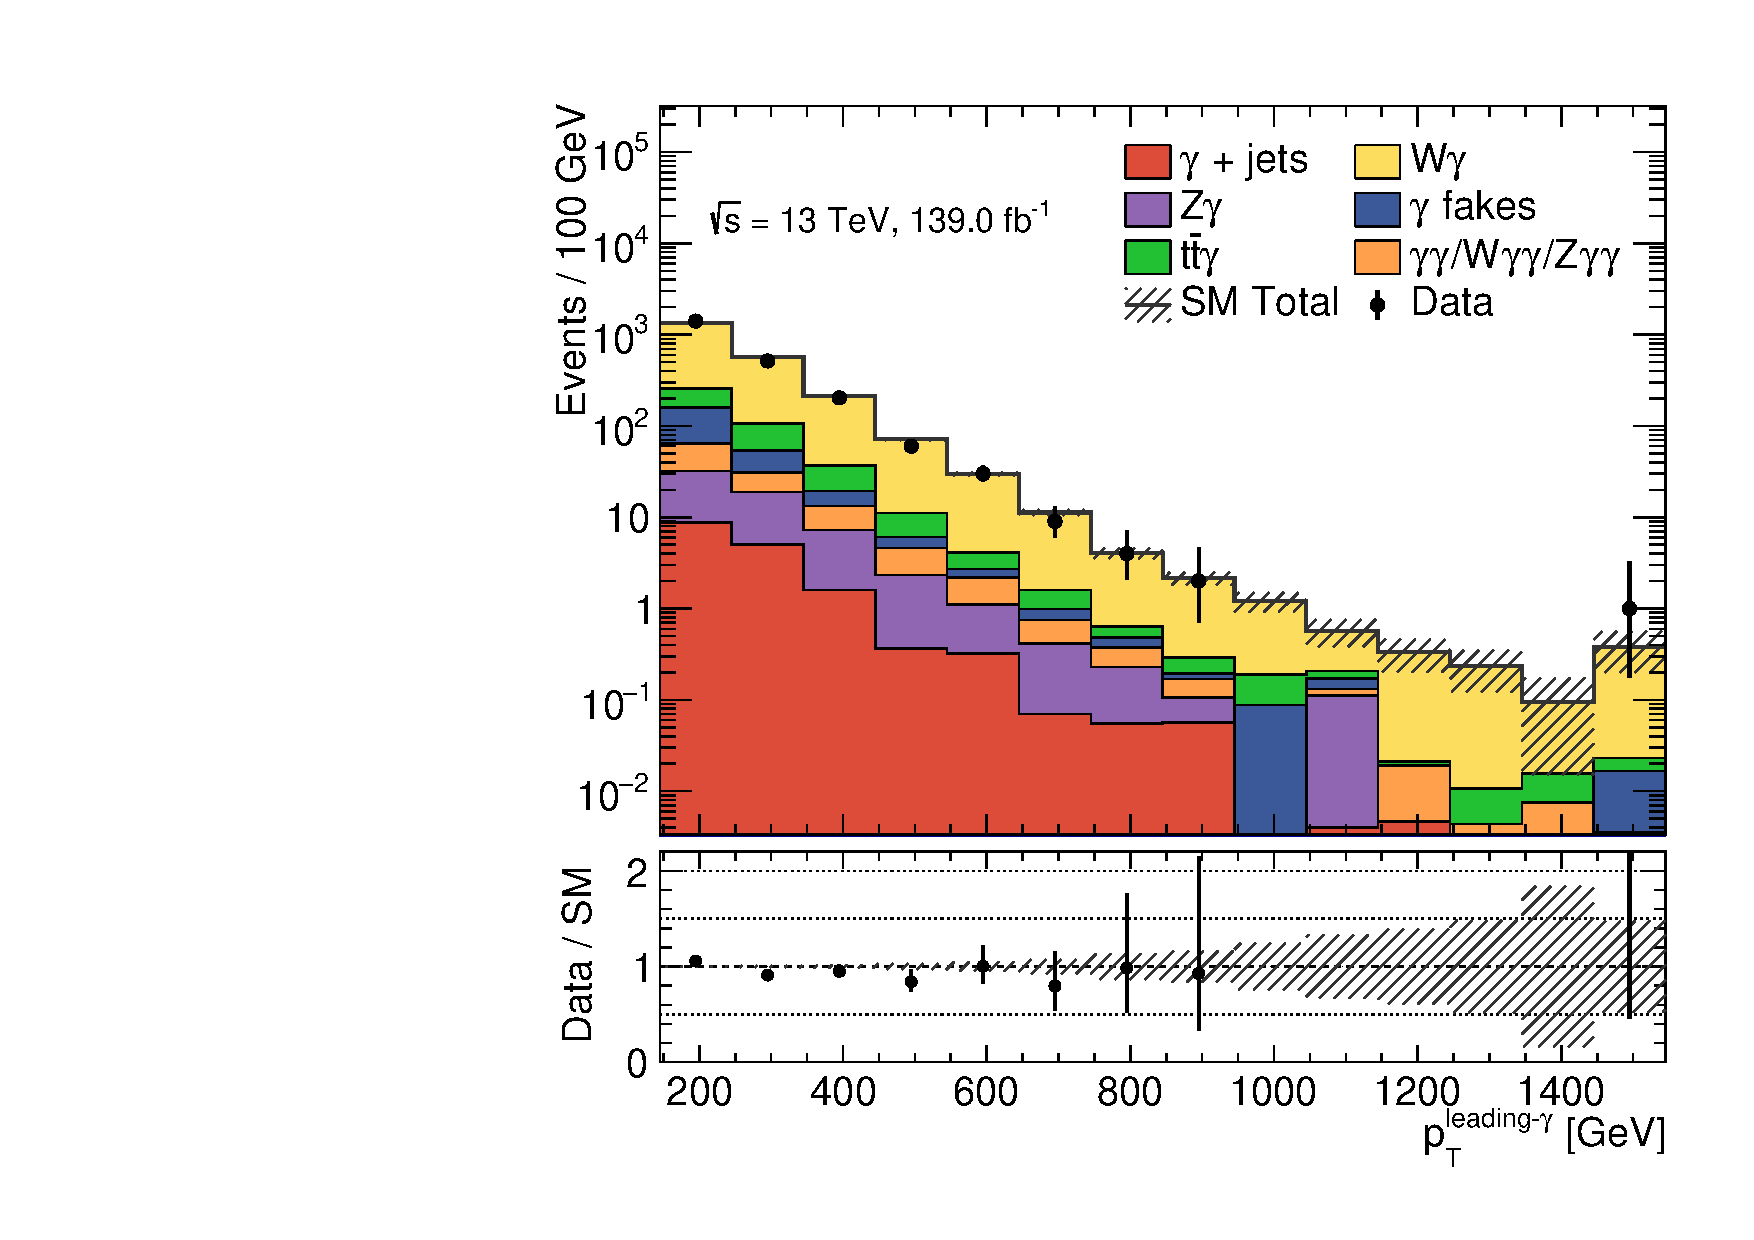
\includegraphics[width=0.32\textwidth]{images/results/fr2_unblind/can_CRW_ph_pt0_afterFit.pdf}
    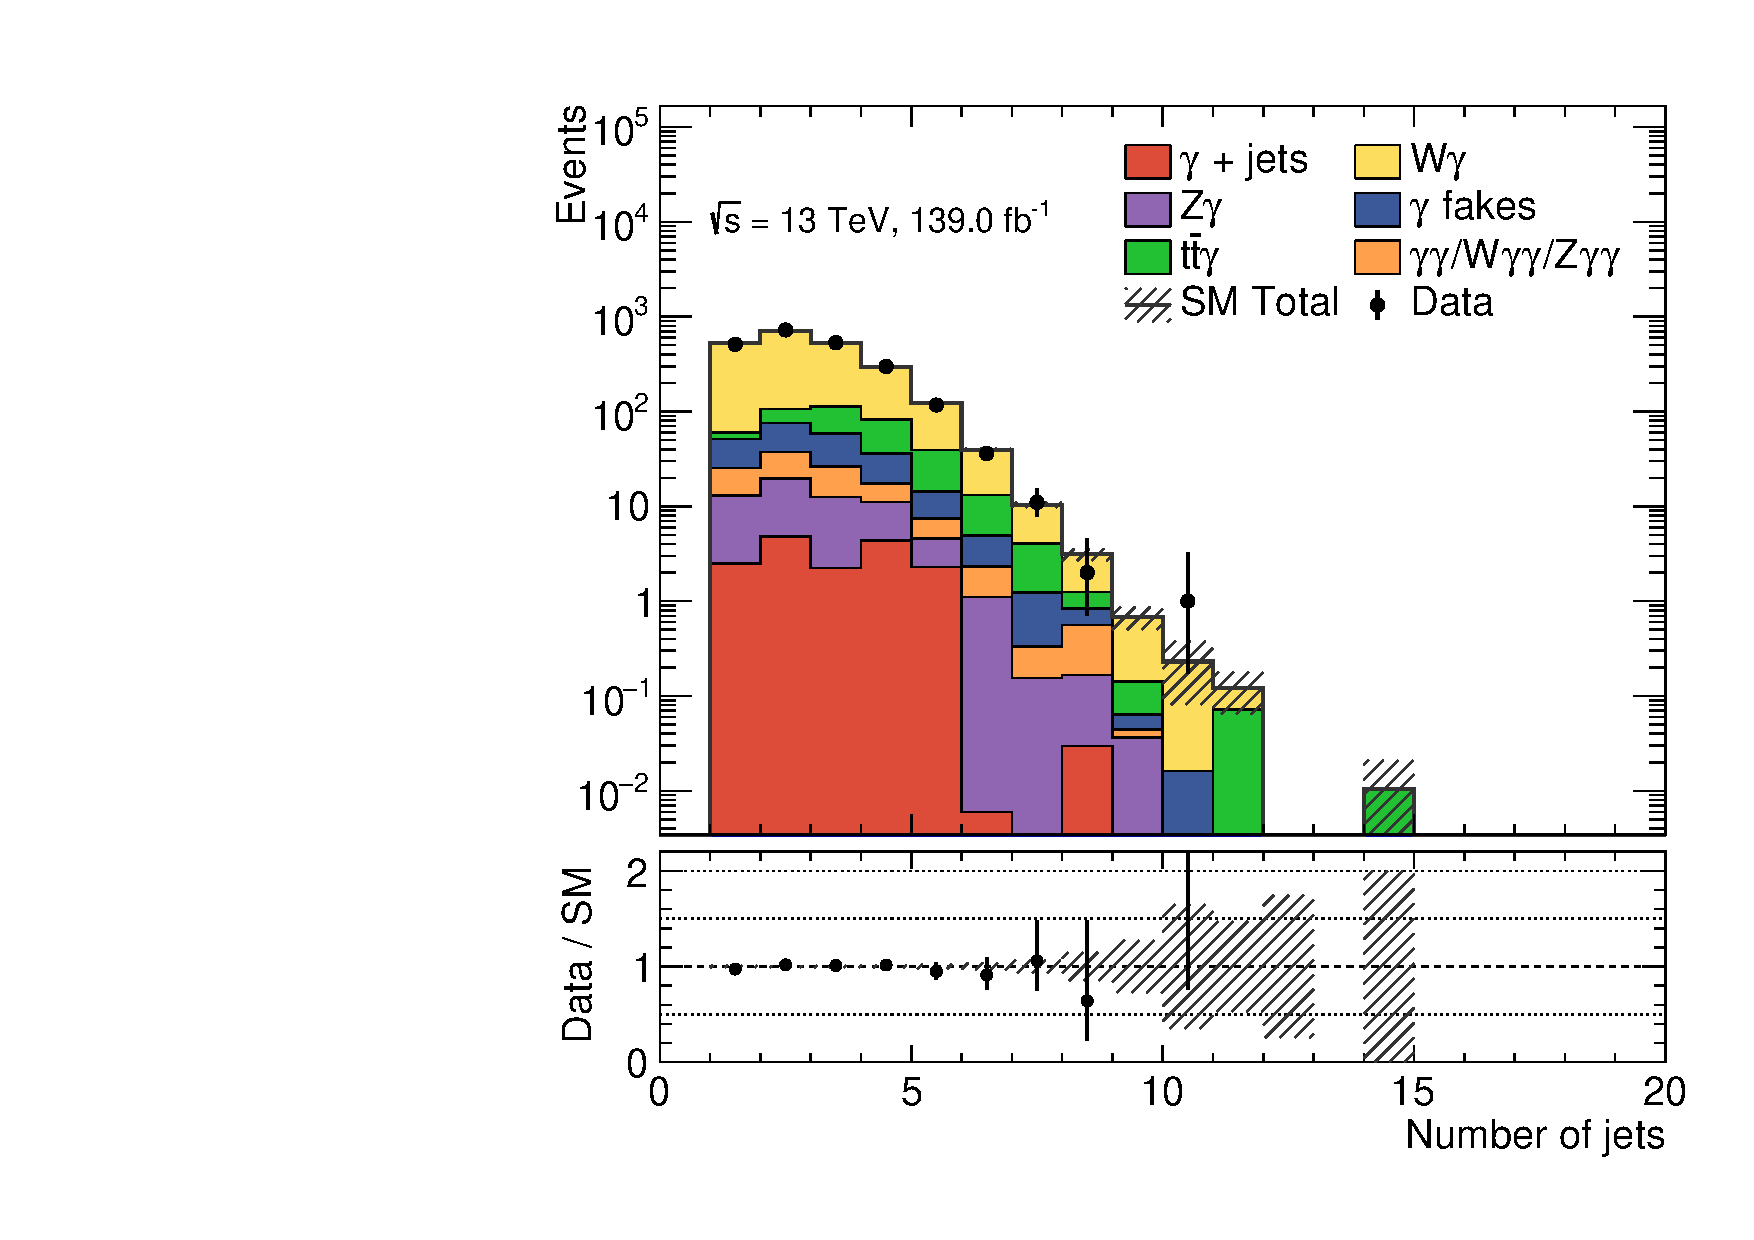
\includegraphics[width=0.32\textwidth]{images/results/fr2_unblind/can_CRW_jet_n_afterFit.pdf}
    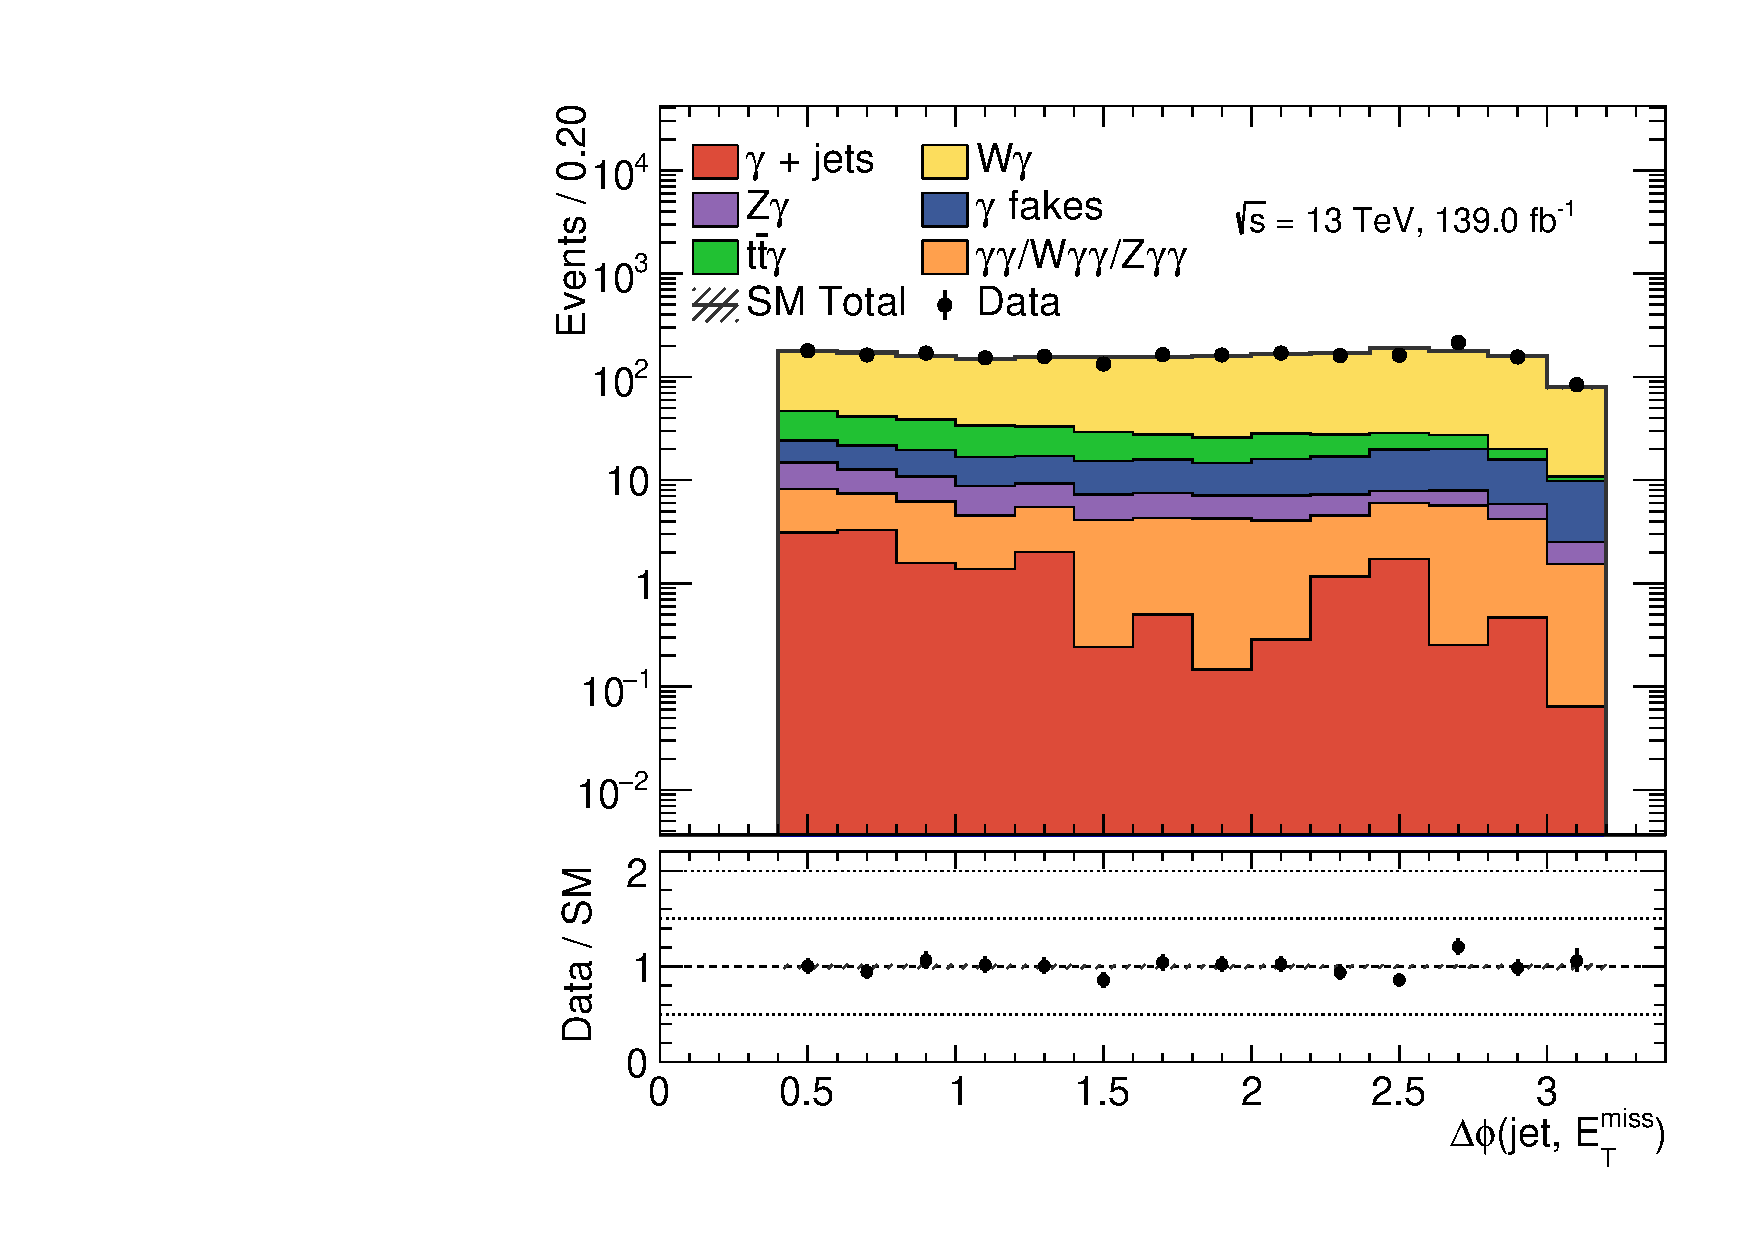
\includegraphics[width=0.32\textwidth]{images/results/fr2_unblind/can_CRW_dphi_jetmet_afterFit.pdf}

    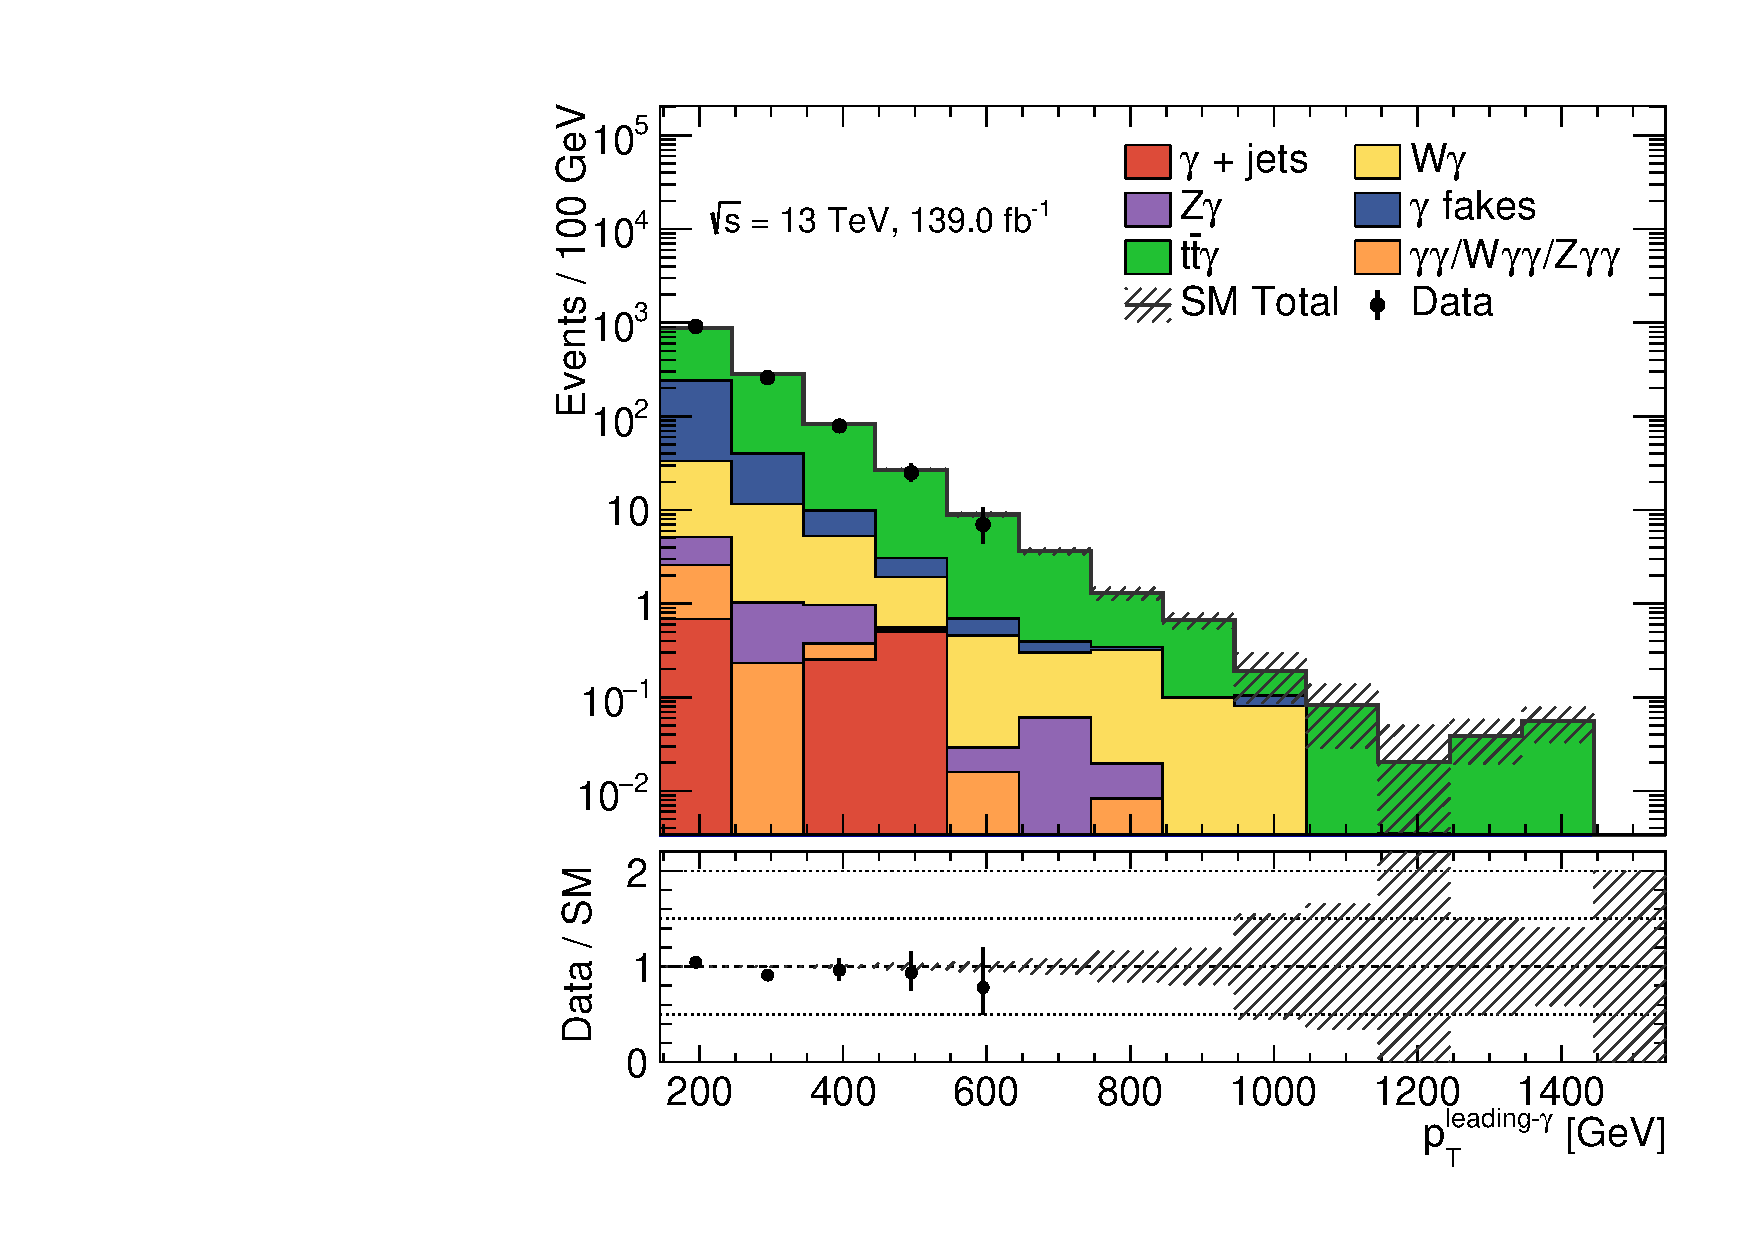
\includegraphics[width=0.32\textwidth]{images/results/fr2_unblind/can_CRT_ph_pt0_afterFit.pdf}
    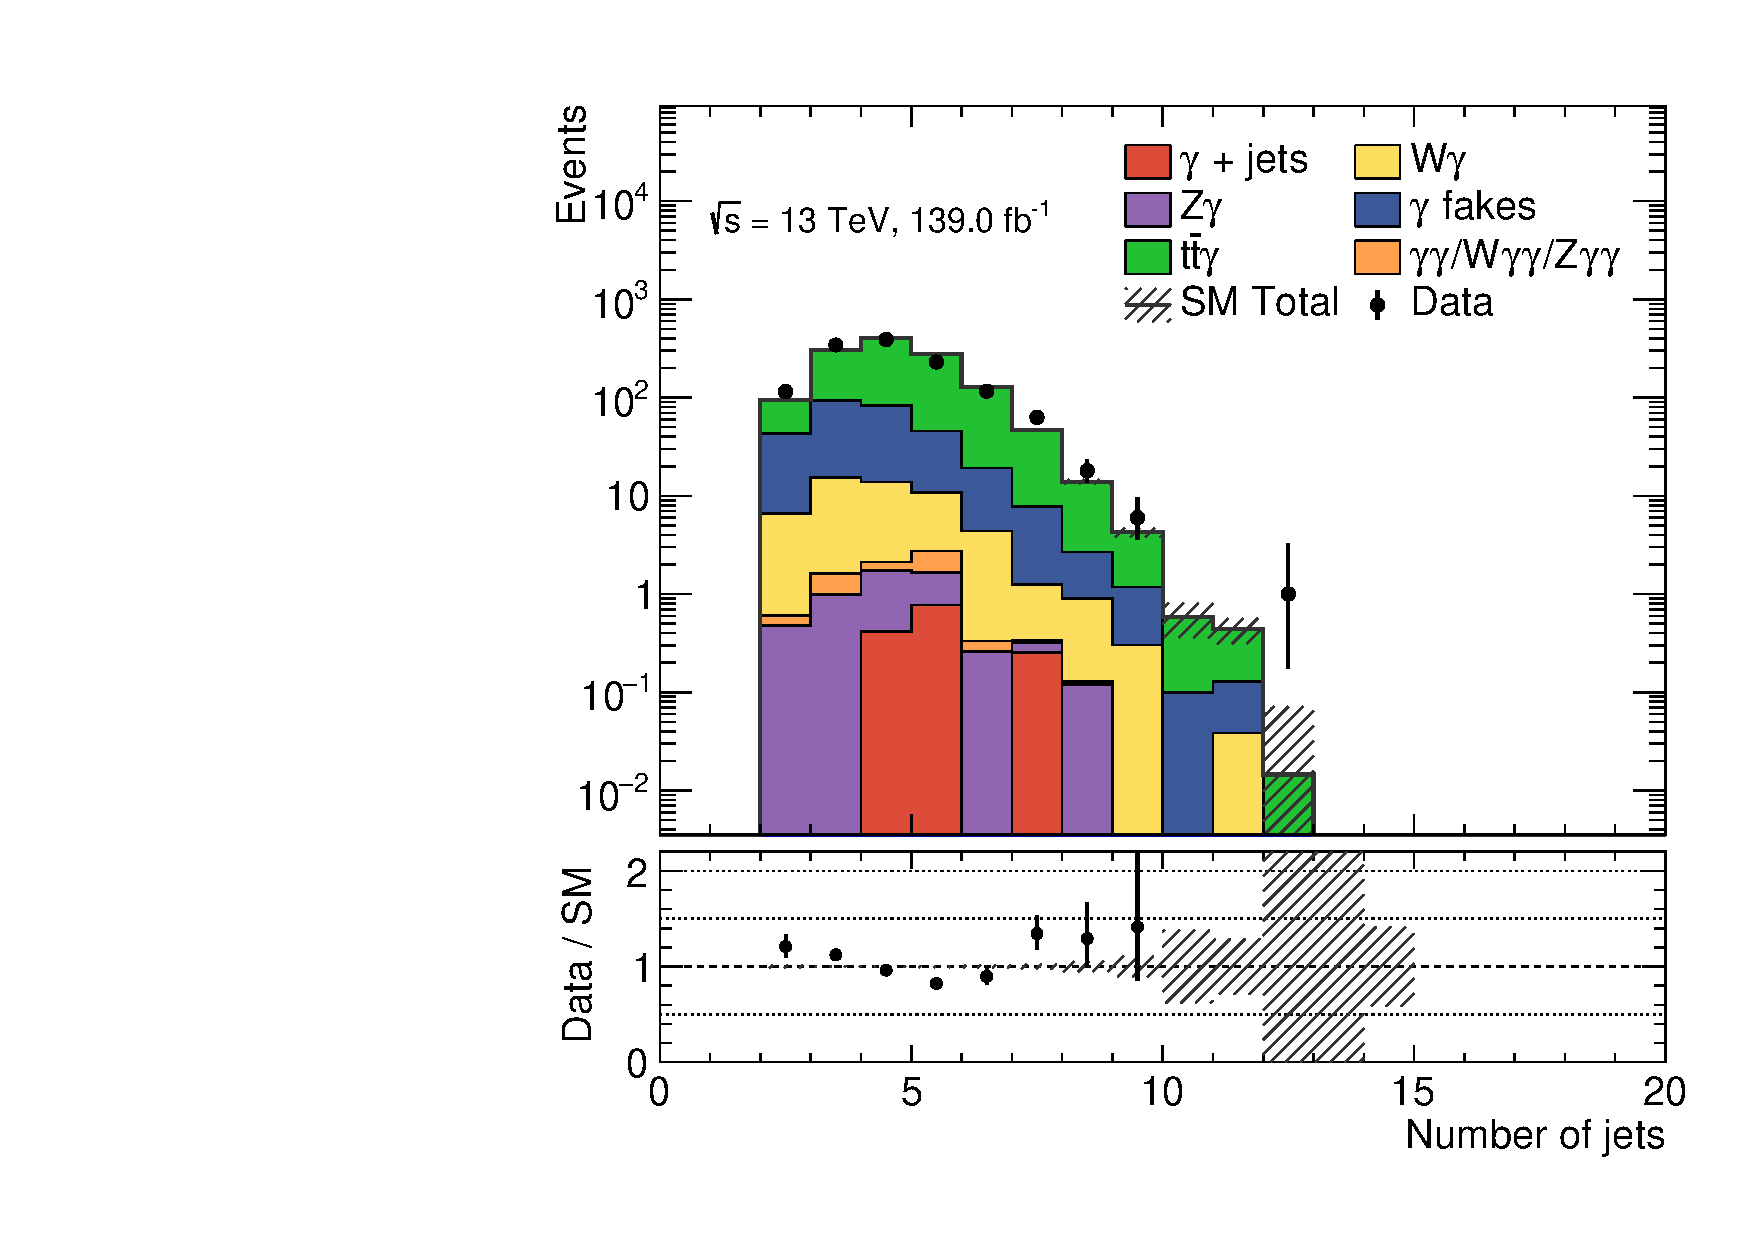
\includegraphics[width=0.32\textwidth]{images/results/fr2_unblind/can_CRT_jet_n_afterFit.pdf}
    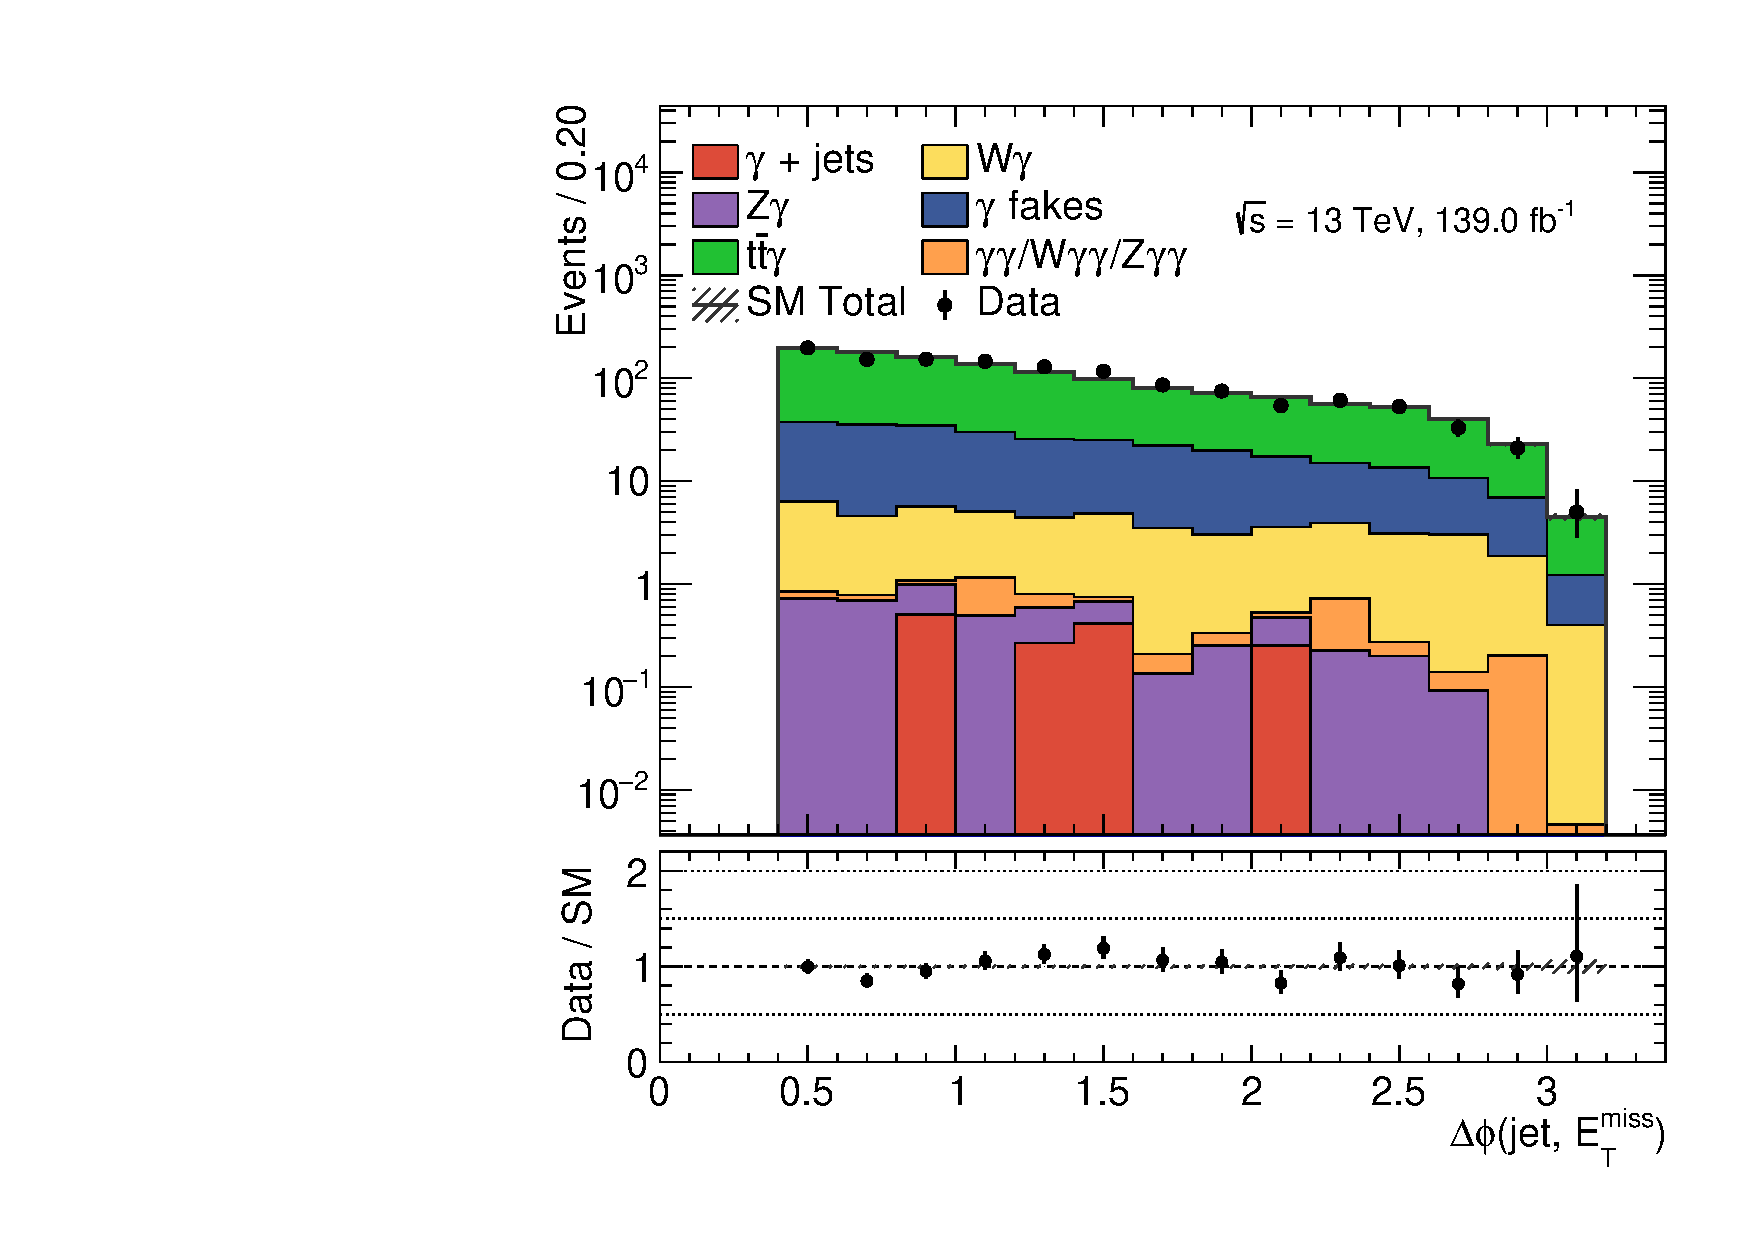
\includegraphics[width=0.32\textwidth]{images/results/fr2_unblind/can_CRT_dphi_jetmet_afterFit.pdf}

    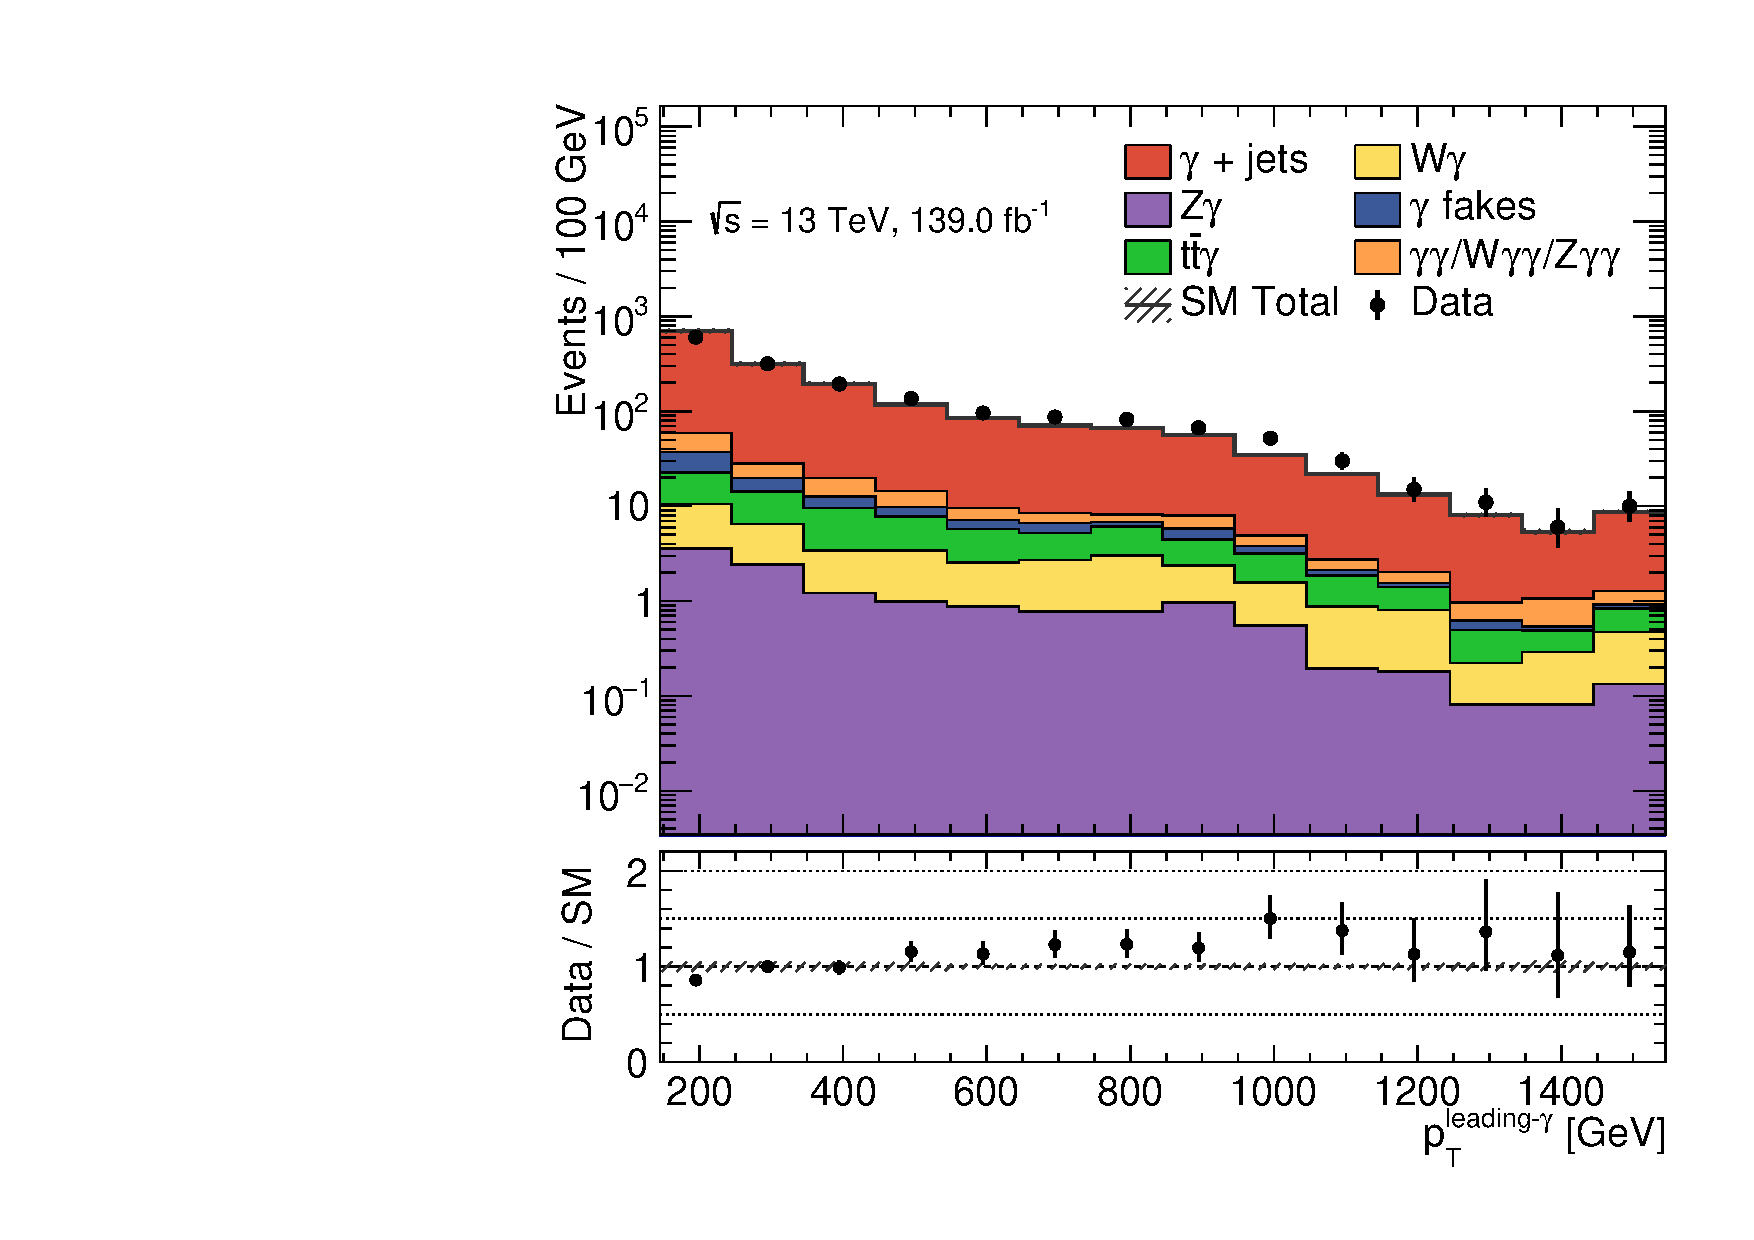
\includegraphics[width=0.32\textwidth]{images/results/fr2_unblind/can_CRQ_ph_pt0_afterFit.pdf}
    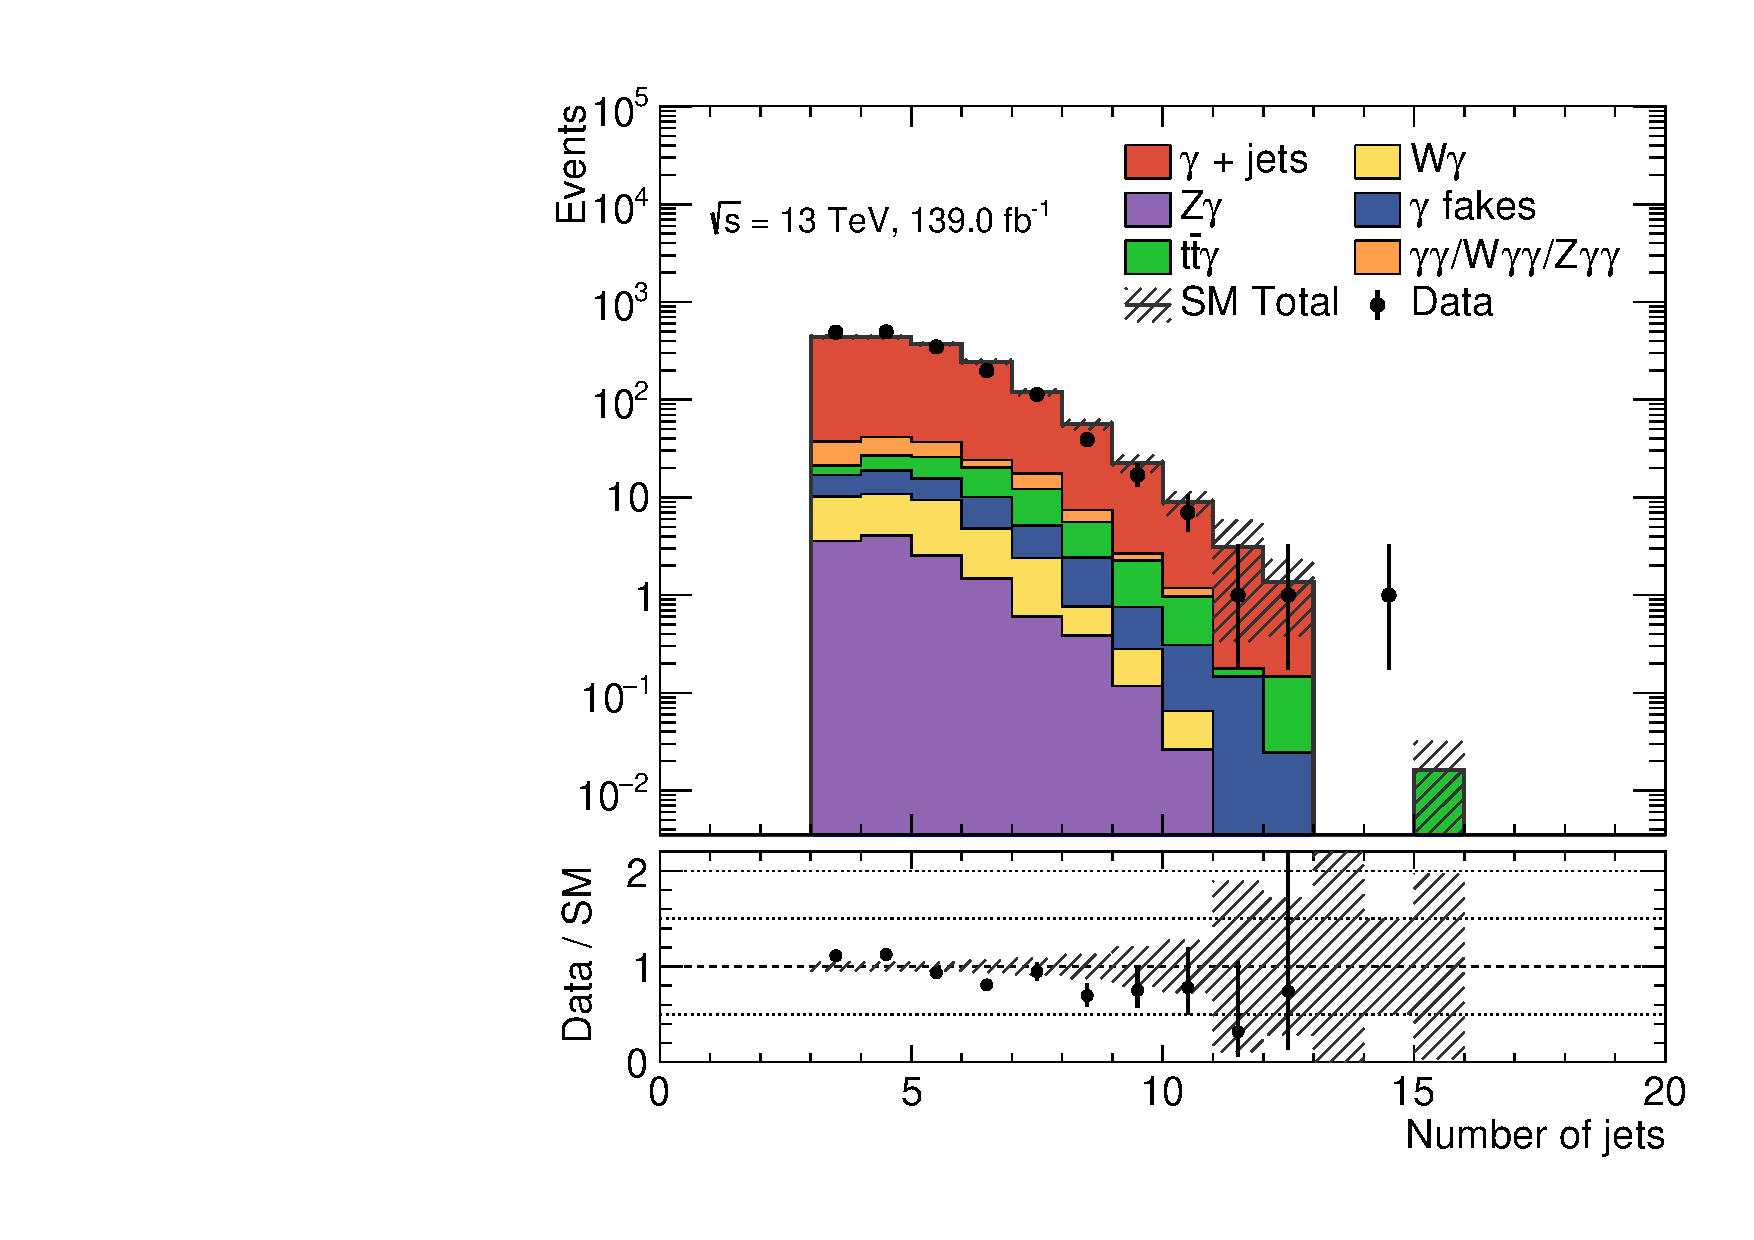
\includegraphics[width=0.32\textwidth]{images/results/fr2_unblind/can_CRQ_jet_n_afterFit.pdf}
    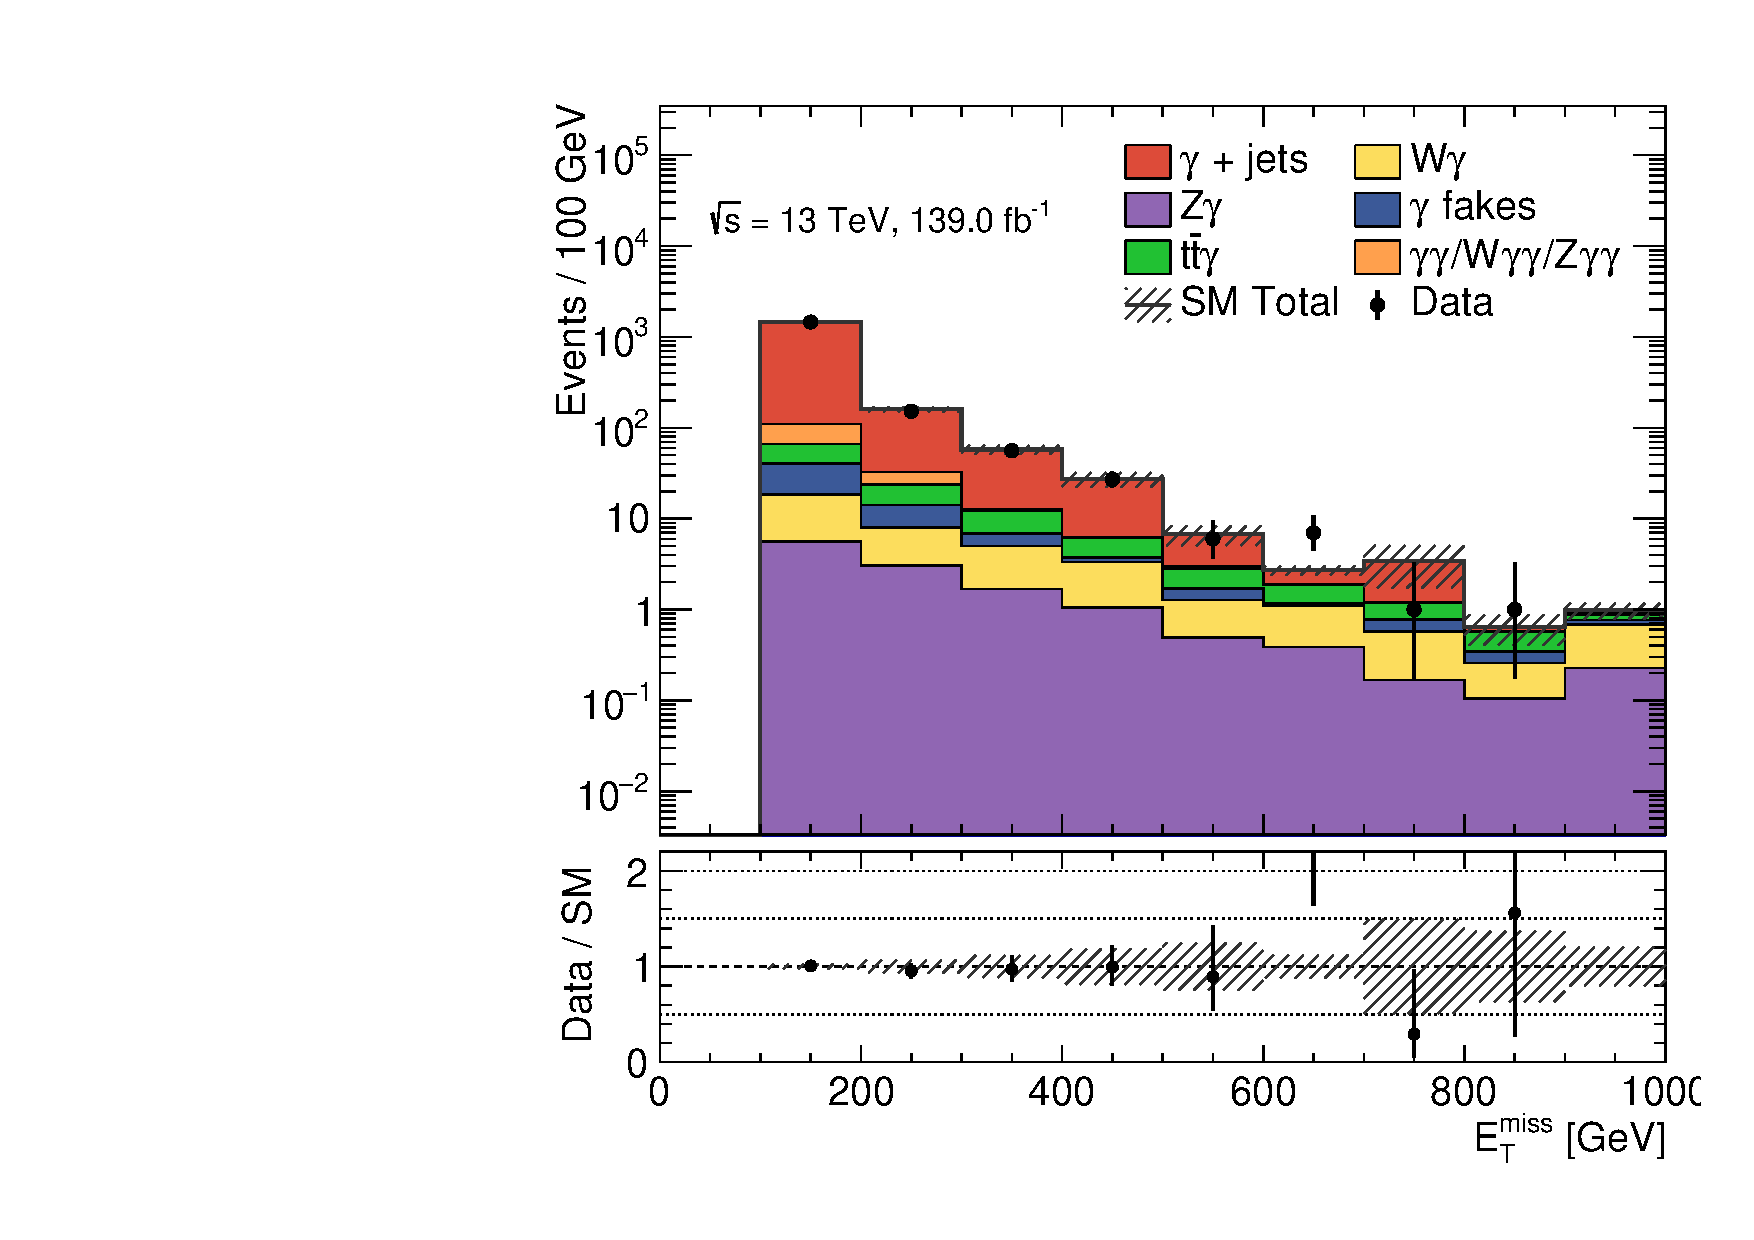
\includegraphics[width=0.32\textwidth]{images/results/fr2_unblind/can_CRQ_met_et_afterFit.pdf}

    \caption{Distribuciones de algunas variables significativas en las regiones de control CRW (arriba), CRT (medio) y CRQ (abajo) luego del ajuste de solo fondo. Las incertidumbre mostradas son sólo estadísticas.}
    \label{fig:cr_dist}
  \end{center}
\end{figure}



\begin{figure}[ht!]

  \centering
  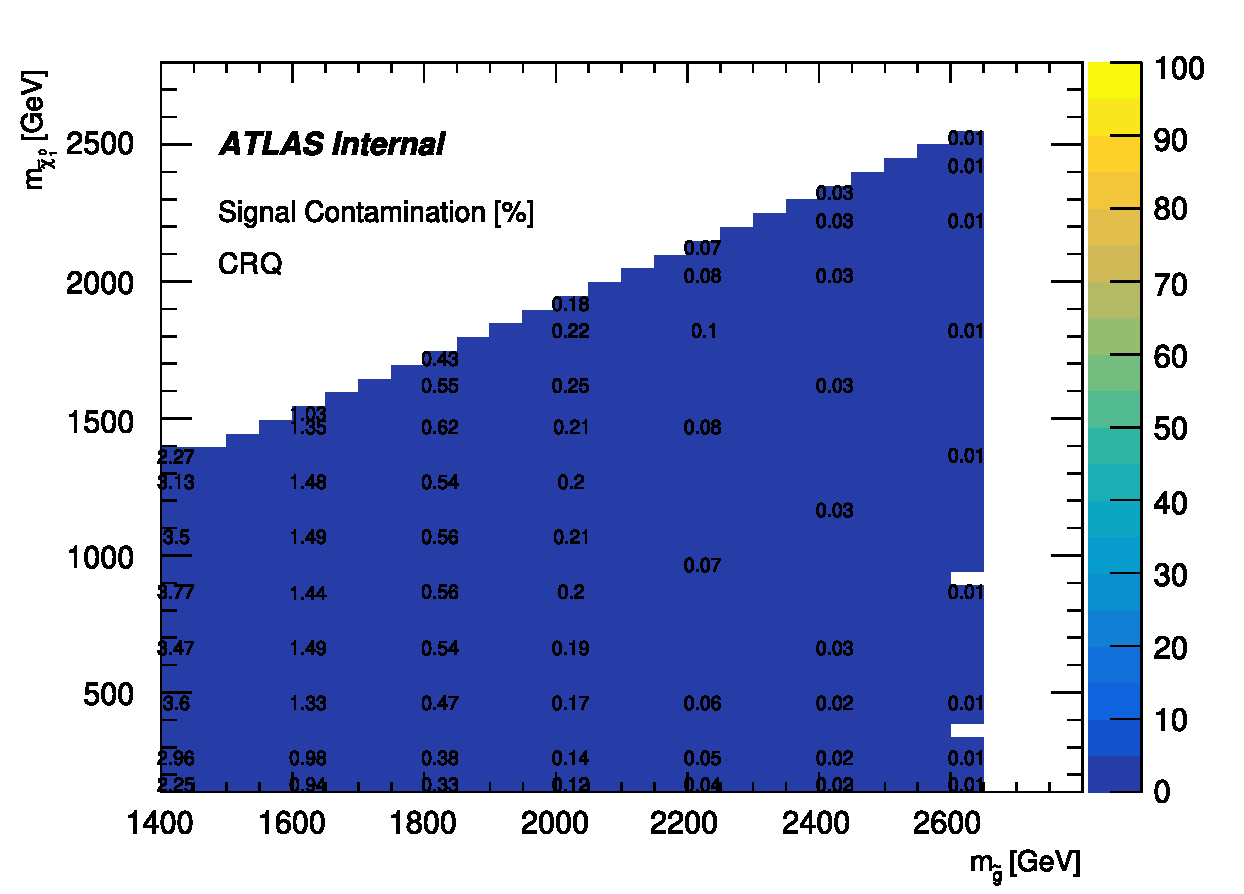
\includegraphics[width=0.32\textwidth]{images/results/signal_contamination_bb_CRQ_139ifb.pdf}
  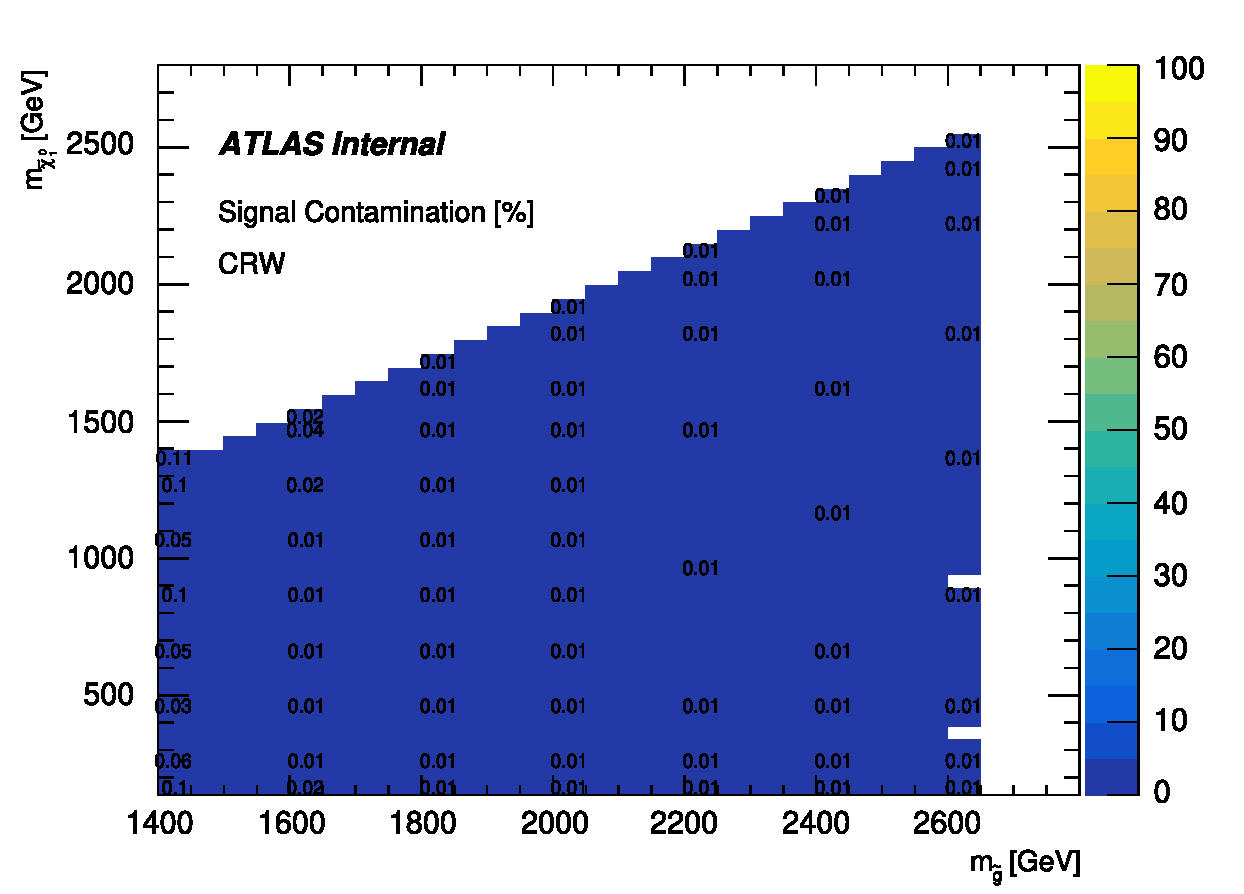
\includegraphics[width=0.32\textwidth]{images/results/signal_contamination_bb_CRW_139ifb.pdf}
  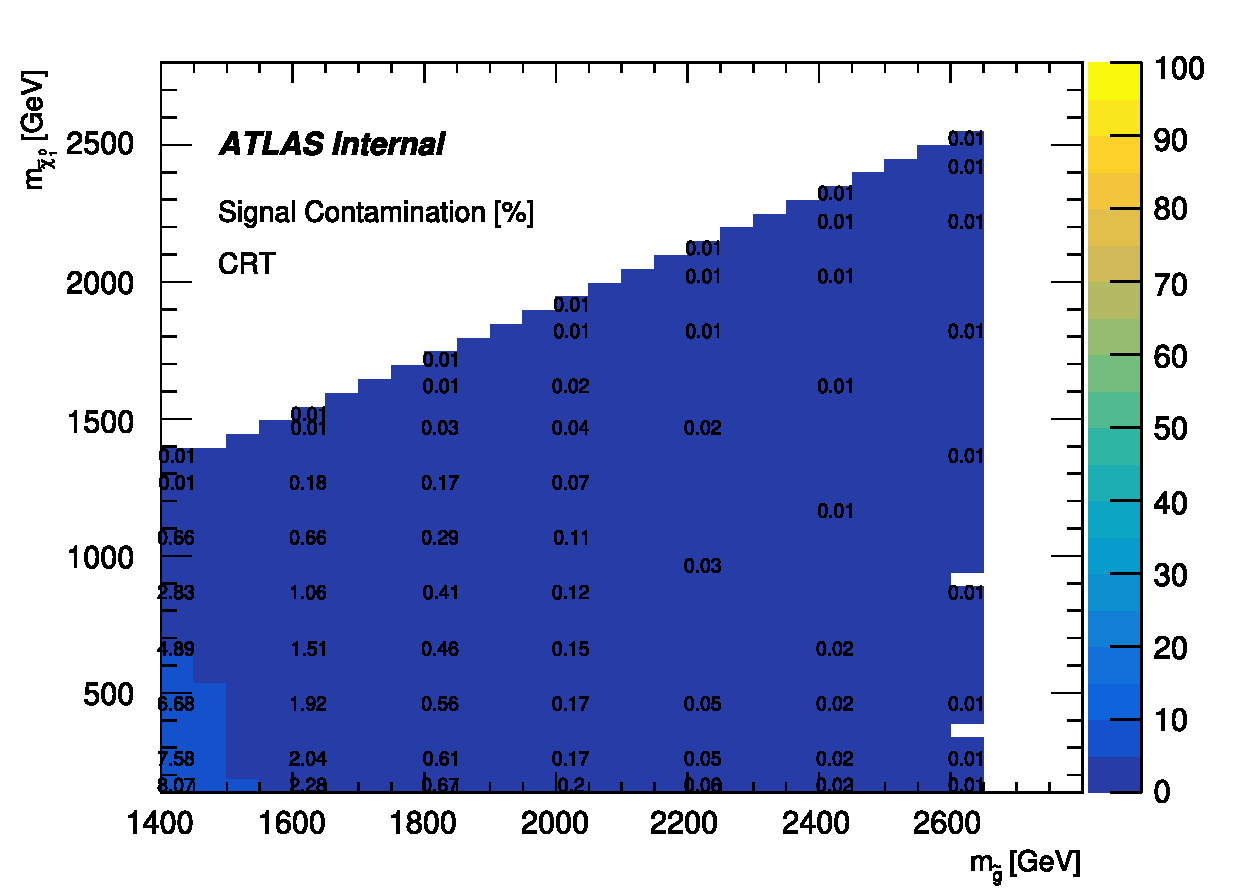
\includegraphics[width=0.32\textwidth]{images/results/signal_contamination_bb_CRT_139ifb.pdf}
  \caption{Contaminación porcentual para cada muestra de señal en las regiones de control CRQ (arriba izquierda), CRW (arriba derecha) y CRT (abajo). La misma se define como la fracción de eventos de señal con respecto al número de eventos de señal más fondo.}
  \label{fig:signal_contamination_CR_bb}

\end{figure}


En las Tablas \ref{tab:bkgonly_result_vrm}, \ref{tab:bkgonly_result_vrm} y \ref{tab:bkgonly_result_vre} se muestran los resultados de la estimación de los fondo en cada región de validación, y algunas de las distribuciones observadas en las mismas se muestran en las Figuras \ref{fig:dist_vrqm_bkgonly} y \ref{fig:dist_vrle_bkgonly}. Se encuentra un buen acuerdo entre los fondos y los datos observados para todas las regiones de validación, dando a entender que la estimación realizada es precisa, y permitiendo continuar con el siguiente paso, donde se comparan los datos observados y las predicciones en las regiones de señal. 


\begin{table}[ht!]
  \centering
  \caption{Estimación de los distintos fondos luego del ajuste de solo fondo en las regiones de validación VRQ, VRM1L, VRM2L, VRM1H y VRM2H.}
  \resizebox{\textwidth}{!}{\begin{tabular}{lrrrrr}
\hline
VRM & VRQ & VRM1L & VRM2L & VRM1H & VRM2H \\
\hline
Observed events & 714 & 127 & 22 & 419 & 51 \\
\hline
Expected SM events & $694.72 \pm 65.58$ & $134.08 \pm 15.99$ & $20.18 \pm 5.01$ & $385.06 \pm 37.21$ & $50.36 \pm 6.53$ \\
\hline
$e\rightarrow\gamma$ fakes & $15.97 \pm 1.17$ & $3.74 \pm 0.38$ & $1.30 \pm 0.19$ & $5.21 \pm 0.48$ & $1.37 \pm 0.20$ \\
$j\rightarrow\gamma$ fakes & $18.04 \pm 3.08$ & $3.59 \pm 0.69$ & $0.35 \pm 0.11$ & $10.38 \pm 1.77$ & $1.28 \pm 0.26$ \\
$\gamma$ + jets & $573.52 \pm 64.46$ & $109.86 \pm 15.13$ & $14.12 \pm 4.26$ & $313.65 \pm 36.88$ & $31.34 \pm 6.10$ \\
$W\gamma$ & $26.99 \pm 1.95$ & $3.67 \pm 0.44$ & $1.11 \pm 0.35$ & $18.59 \pm 1.24$ & $6.79 \pm 0.86$ \\
$Z(\rightarrow\ell\ell)\gamma$ & $2.09 \pm 0.60$ & $0.29 \pm 0.11$ & $0.14 \pm 0.07$ & $1.09 \pm 0.35$ & $0.28 \pm 0.17$ \\
$Z(\rightarrow\nu\nu)\gamma$ & $9.65 \pm 2.67$ & $0.89 \pm 0.26$ & $0.45 \pm 0.16$ & $5.94 \pm 1.64$ & $2.63 \pm 0.75$ \\
$t\bar{t}\gamma$ & $23.91 \pm 1.80$ & $9.80 \pm 1.02$ & $2.34 \pm 0.57$ & $15.70 \pm 1.17$ & $4.39 \pm 0.51$ \\
$\gamma\gamma / W\gamma\gamma / Z\gamma\gamma$ & $24.55 \pm 1.97$ & $2.23 \pm 0.77$ & $0.37 \pm 0.12$ & $14.50 \pm 1.32$ & $2.29 \pm 0.42$ \\
\hline
\end{tabular}
}
  %\resizebox{\textwidth}{!}{\begin{tabular}{lrrrrr}
\hline
VRM & VRQ & VRM1L & VRM2L & VRM1H & VRM2H \\
\hline
Observed events & 714 & 127 & 22 & 419 & 51 \\
\hline
Expected SM events & $694.72 \pm 65.58$ & $134.08 \pm 15.99$ & $20.18 \pm 5.01$ & $385.06 \pm 37.21$ & $50.36 \pm 6.53$ \\
\hline
$e\rightarrow\gamma$ fakes & $15.97 \pm 1.17$ & $3.74 \pm 0.38$ & $1.30 \pm 0.19$ & $5.21 \pm 0.48$ & $1.37 \pm 0.20$ \\
$j\rightarrow\gamma$ fakes & $18.04 \pm 3.08$ & $3.59 \pm 0.69$ & $0.35 \pm 0.11$ & $10.38 \pm 1.77$ & $1.28 \pm 0.26$ \\
$\gamma$ + jets & $573.52 \pm 64.46$ & $109.86 \pm 15.13$ & $14.12 \pm 4.26$ & $313.65 \pm 36.88$ & $31.34 \pm 6.10$ \\
$W\gamma$ & $26.99 \pm 1.95$ & $3.67 \pm 0.44$ & $1.11 \pm 0.35$ & $18.59 \pm 1.24$ & $6.79 \pm 0.86$ \\
$Z(\rightarrow\ell\ell)\gamma$ & $2.09 \pm 0.60$ & $0.29 \pm 0.11$ & $0.14 \pm 0.07$ & $1.09 \pm 0.35$ & $0.28 \pm 0.17$ \\
$Z(\rightarrow\nu\nu)\gamma$ & $9.65 \pm 2.67$ & $0.89 \pm 0.26$ & $0.45 \pm 0.16$ & $5.94 \pm 1.64$ & $2.63 \pm 0.75$ \\
$t\bar{t}\gamma$ & $23.91 \pm 1.80$ & $9.80 \pm 1.02$ & $2.34 \pm 0.57$ & $15.70 \pm 1.17$ & $4.39 \pm 0.51$ \\
$\gamma\gamma / W\gamma\gamma / Z\gamma\gamma$ & $24.55 \pm 1.97$ & $2.23 \pm 0.77$ & $0.37 \pm 0.12$ & $14.50 \pm 1.32$ & $2.29 \pm 0.42$ \\
\hline
\end{tabular}
}
  \label{tab:bkgonly_result_vrm}
\end{table}


\begin{table}[ht!]
  \centering
  \caption{Estimación de los distintos fondos luego del ajuste de solo fondo en las regiones de validación VRL1, VRL2, VRL3 y VRL4.}
  \resizebox{\textwidth}{!}{\begin{tabular}{lrrrr}
\hline
VRL & VRL1 & VRL2 & VRL3 & VRL4 \\
\hline
Observed events & 1731 & 257 & 699 & 52 \\
\hline
Expected SM events & $1686.63 \pm 48.08$ & $252.19 \pm 11.37$ & $734.90 \pm 23.54$ & $51.54 \pm 2.88$ \\
\hline
$e\rightarrow\gamma$ fakes & $151.56 \pm 9.46$ & $20.50 \pm 1.45$ & $51.82 \pm 3.38$ & $4.48 \pm 0.44$ \\
$j\rightarrow\gamma$ fakes & $32.36 \pm 4.88$ & $3.67 \pm 0.62$ & $25.84 \pm 9.28$ & $1.08 \pm 0.38$ \\
$\gamma$ + jets & $21.85 \pm 6.65$ & $4.75 \pm 1.14$ & $1.81 \pm 0.57$ & $0.15_{-0.15}^{+0.16}$ \\
$W\gamma$ & $877.59 \pm 44.21$ & $144.49 \pm 9.04$ & $430.59 \pm 22.23$ & $17.23 \pm 1.52$ \\
$Z(\rightarrow\ell\ell)\gamma$ & $52.81 \pm 14.45$ & $10.62 \pm 3.00$ & $7.39 \pm 2.01$ & $0.74 \pm 0.25$ \\
$Z(\rightarrow\nu\nu)\gamma$ & $0.03 \pm 0.01$ & $0.01 \pm 0.00$ & $0.03 \pm 0.01$ & $0.00 \pm 0.00$ \\
$t\bar{t}\gamma$ & $510.48 \pm 27.74$ & $59.19 \pm 3.62$ & $203.73 \pm 11.06$ & $26.91 \pm 1.97$ \\
$\gamma\gamma / W\gamma\gamma / Z\gamma\gamma$ & $39.95 \pm 1.73$ & $8.96 \pm 0.70$ & $13.70 \pm 0.61$ & $0.95 \pm 0.06$ \\
\hline
\end{tabular}
}
  %\resizebox{\textwidth}{!}{\begin{tabular}{lrrrr}
\hline
VRL & VRL1 & VRL2 & VRL3 & VRL4 \\
\hline
Observed events & 1731 & 257 & 699 & 52 \\
\hline
Expected SM events & $1686.63 \pm 48.08$ & $252.19 \pm 11.37$ & $734.90 \pm 23.54$ & $51.54 \pm 2.88$ \\
\hline
$e\rightarrow\gamma$ fakes & $151.56 \pm 9.46$ & $20.50 \pm 1.45$ & $51.82 \pm 3.38$ & $4.48 \pm 0.44$ \\
$j\rightarrow\gamma$ fakes & $32.36 \pm 4.88$ & $3.67 \pm 0.62$ & $25.84 \pm 9.28$ & $1.08 \pm 0.38$ \\
$\gamma$ + jets & $21.85 \pm 6.65$ & $4.75 \pm 1.14$ & $1.81 \pm 0.57$ & $0.15_{-0.15}^{+0.16}$ \\
$W\gamma$ & $877.59 \pm 44.21$ & $144.49 \pm 9.04$ & $430.59 \pm 22.23$ & $17.23 \pm 1.52$ \\
$Z(\rightarrow\ell\ell)\gamma$ & $52.81 \pm 14.45$ & $10.62 \pm 3.00$ & $7.39 \pm 2.01$ & $0.74 \pm 0.25$ \\
$Z(\rightarrow\nu\nu)\gamma$ & $0.03 \pm 0.01$ & $0.01 \pm 0.00$ & $0.03 \pm 0.01$ & $0.00 \pm 0.00$ \\
$t\bar{t}\gamma$ & $510.48 \pm 27.74$ & $59.19 \pm 3.62$ & $203.73 \pm 11.06$ & $26.91 \pm 1.97$ \\
$\gamma\gamma / W\gamma\gamma / Z\gamma\gamma$ & $39.95 \pm 1.73$ & $8.96 \pm 0.70$ & $13.70 \pm 0.61$ & $0.95 \pm 0.06$ \\
\hline
\end{tabular}
}
  \label{tab:bkgonly_result_vrl}
\end{table}

\begin{table}[ht!]
  \centering
  \caption{Estimación de los distintos fondos luego del ajuste de solo fondo en la VRE.}
  \begin{tabular}{lr}
\hline
Fakes VR & VRE \\
\hline
Observed events & 520 \\
\hline
Expected SM events & $550.63 \pm 31.61$ \\
\hline
$e\rightarrow\gamma$ fakes & $418.40 \pm 25.79$ \\
$j\rightarrow\gamma$ fakes & $46.25 \pm 15.98$ \\
$\gamma$ + jets & $7.59 \pm 2.06$ \\
$W\gamma$ & $48.36 \pm 7.79$ \\
$Z(\rightarrow\ell\ell)\gamma$ & $0.45 \pm 0.11$ \\
$Z(\rightarrow\nu\nu)\gamma$ & $4.54 \pm 1.15$ \\
$t\bar{t}\gamma$ & $23.10 \pm 2.37$ \\
$\gamma\gamma / W\gamma\gamma / Z\gamma\gamma$ & $1.95 \pm 0.30$ \\
\hline
\end{tabular}

  %\begin{tabular}{lr}
\hline
Fakes VR & VRE \\
\hline
Observed events & 520 \\
\hline
Expected SM events & $550.63 \pm 31.61$ \\
\hline
$e\rightarrow\gamma$ fakes & $418.40 \pm 25.79$ \\
$j\rightarrow\gamma$ fakes & $46.25 \pm 15.98$ \\
$\gamma$ + jets & $7.59 \pm 2.06$ \\
$W\gamma$ & $48.36 \pm 7.79$ \\
$Z(\rightarrow\ell\ell)\gamma$ & $0.45 \pm 0.11$ \\
$Z(\rightarrow\nu\nu)\gamma$ & $4.54 \pm 1.15$ \\
$t\bar{t}\gamma$ & $23.10 \pm 2.37$ \\
$\gamma\gamma / W\gamma\gamma / Z\gamma\gamma$ & $1.95 \pm 0.30$ \\
\hline
\end{tabular}

  \label{tab:bkgonly_result_vre}
\end{table}

\begin{figure}[ht!]
  \centering

    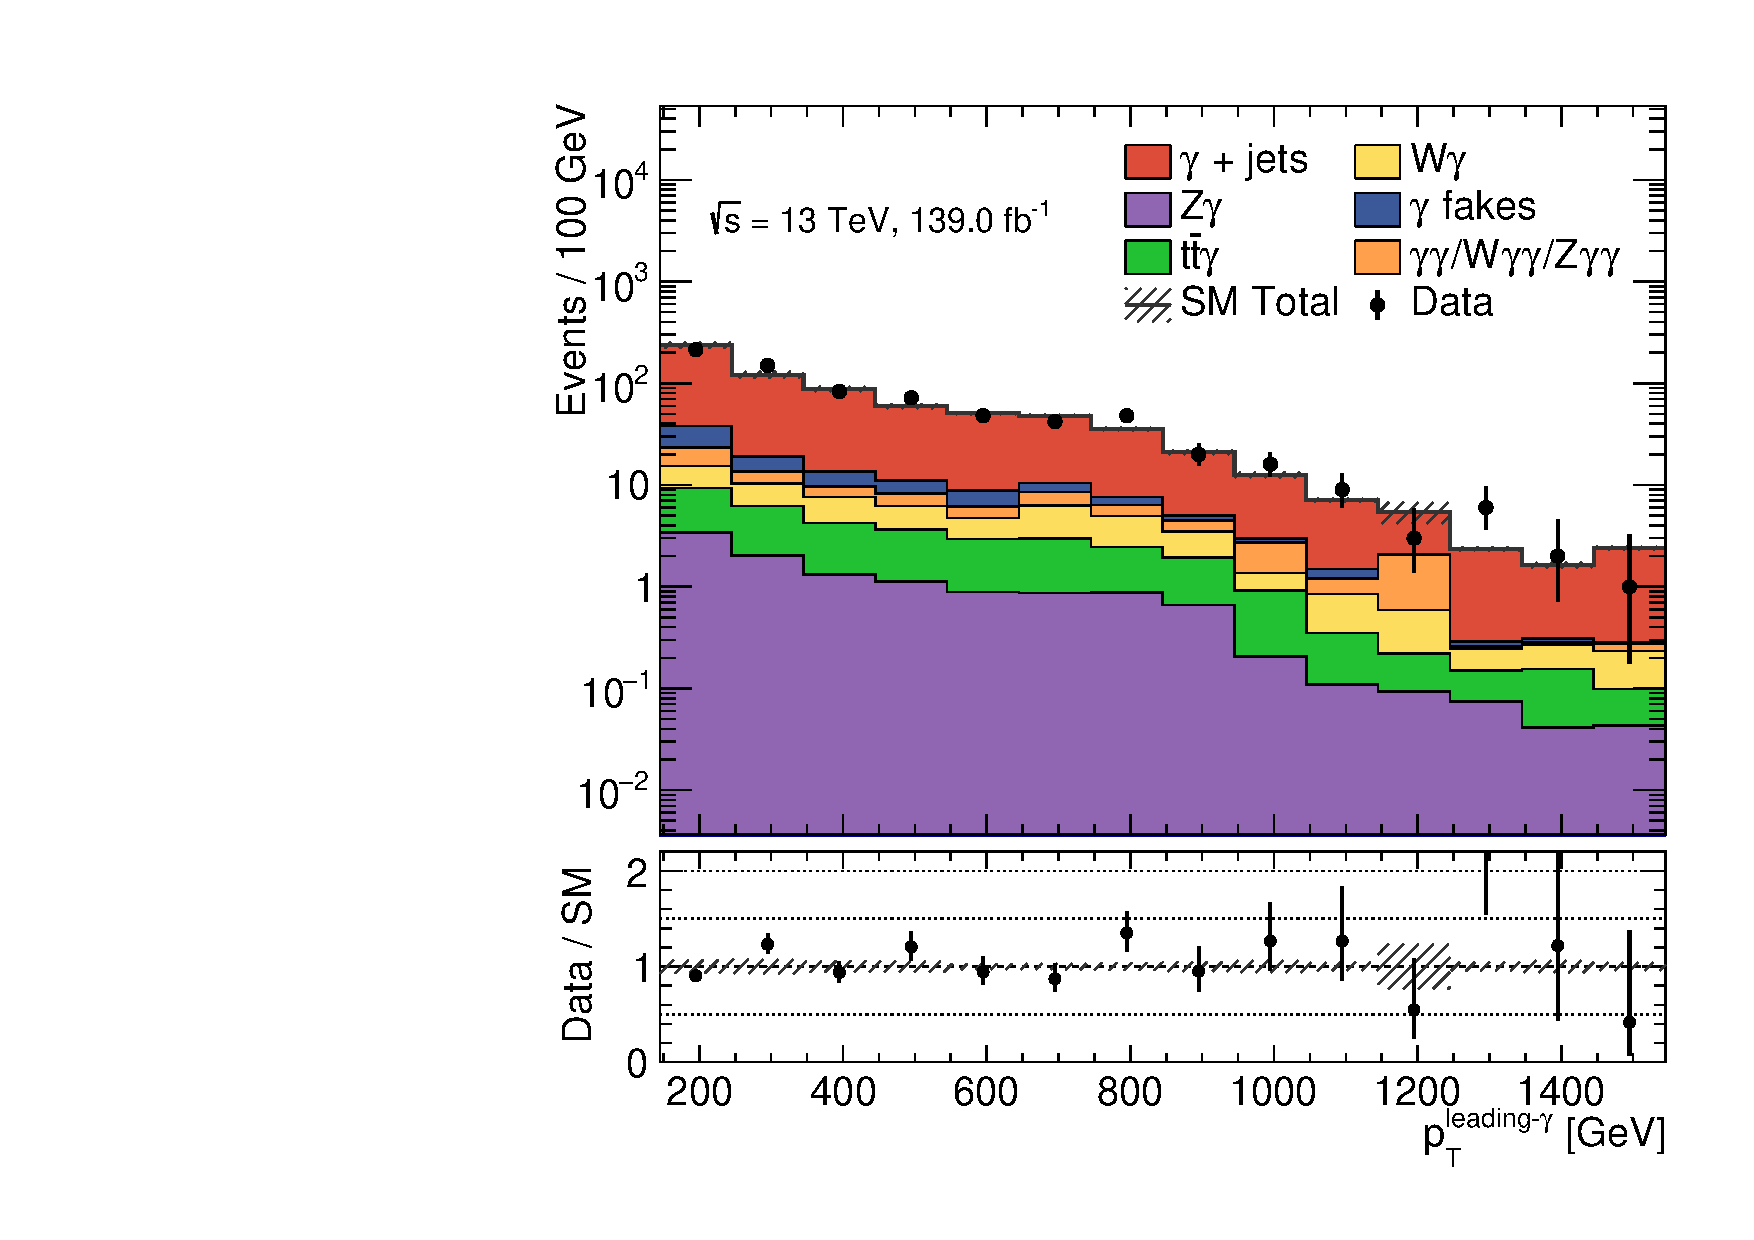
\includegraphics[width=0.32\textwidth]{images/results/fr2_unblind/can_VRQ_ph_pt0_afterFit.pdf}
    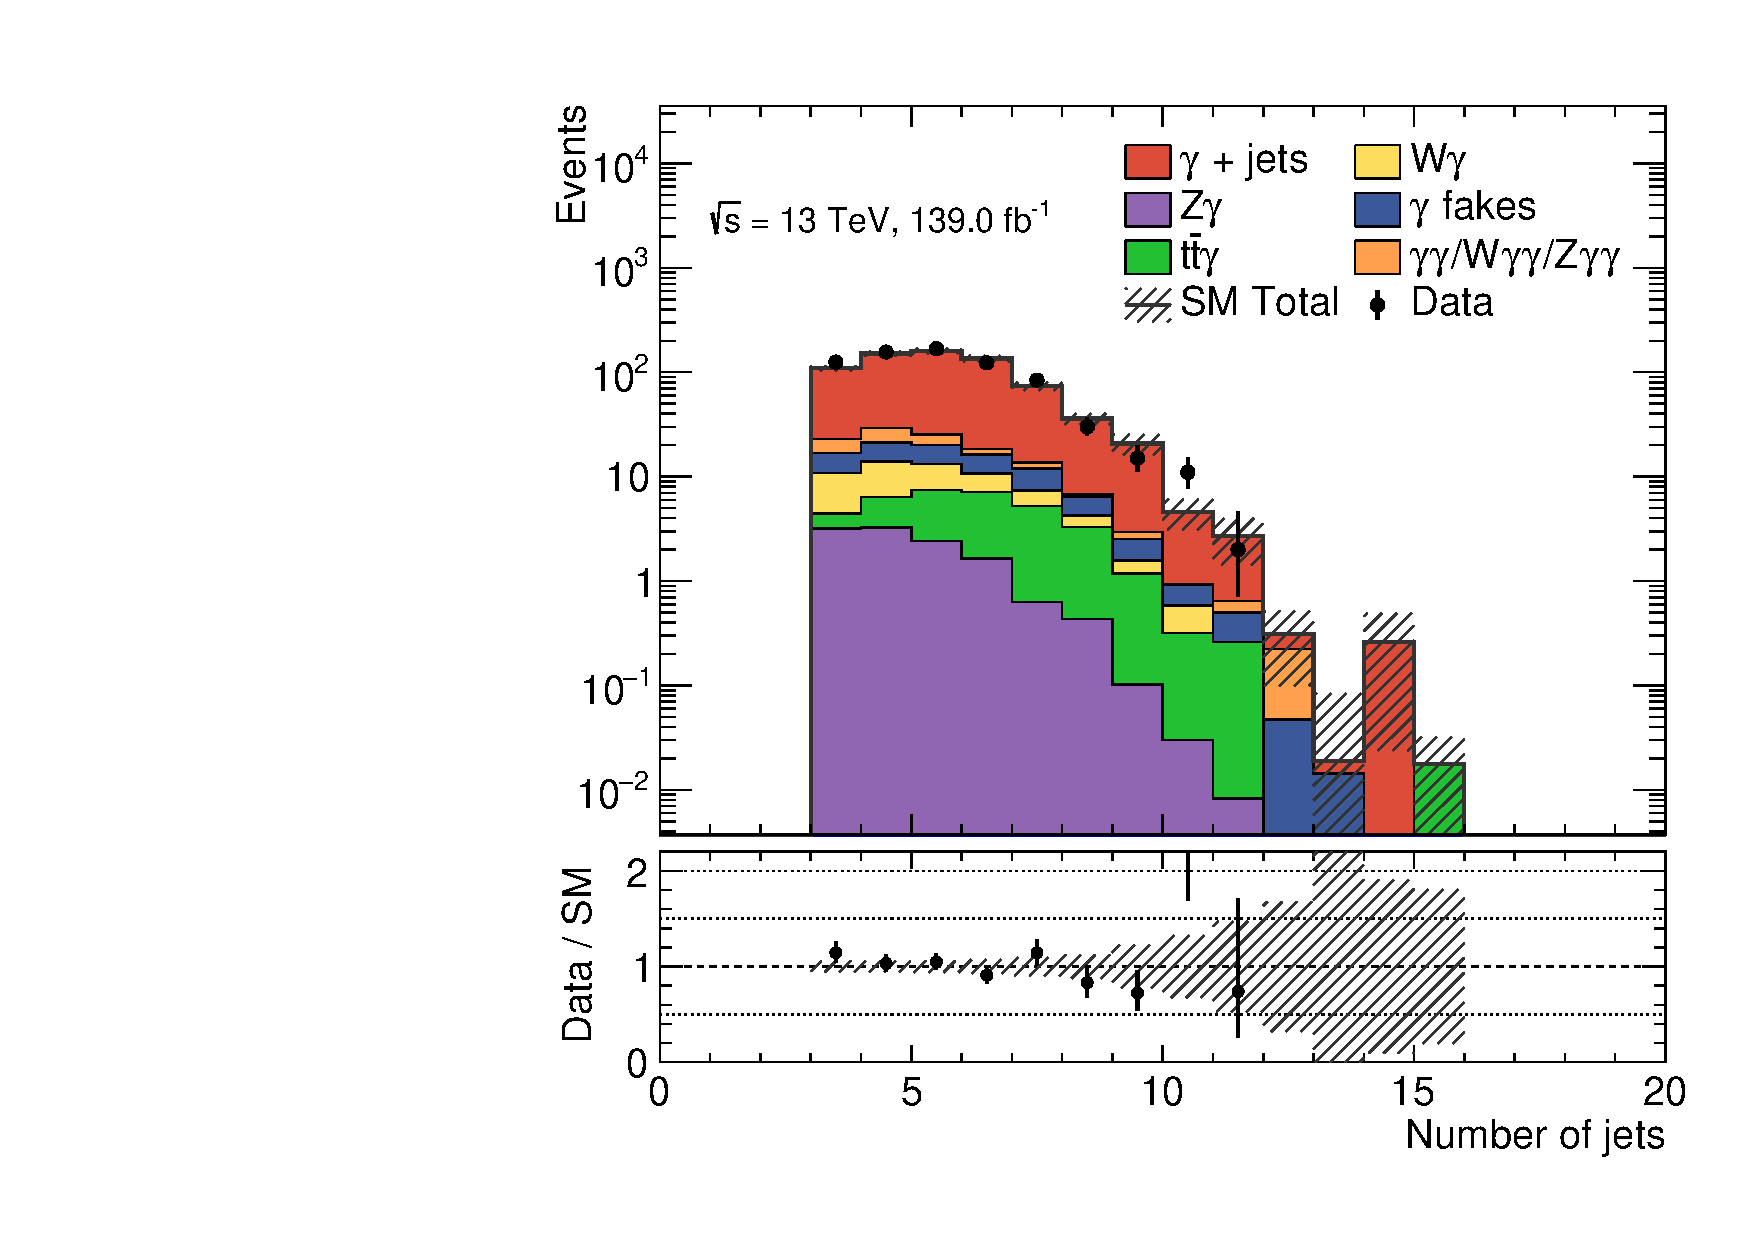
\includegraphics[width=0.32\textwidth]{images/results/fr2_unblind/can_VRQ_jet_n_afterFit.pdf}
    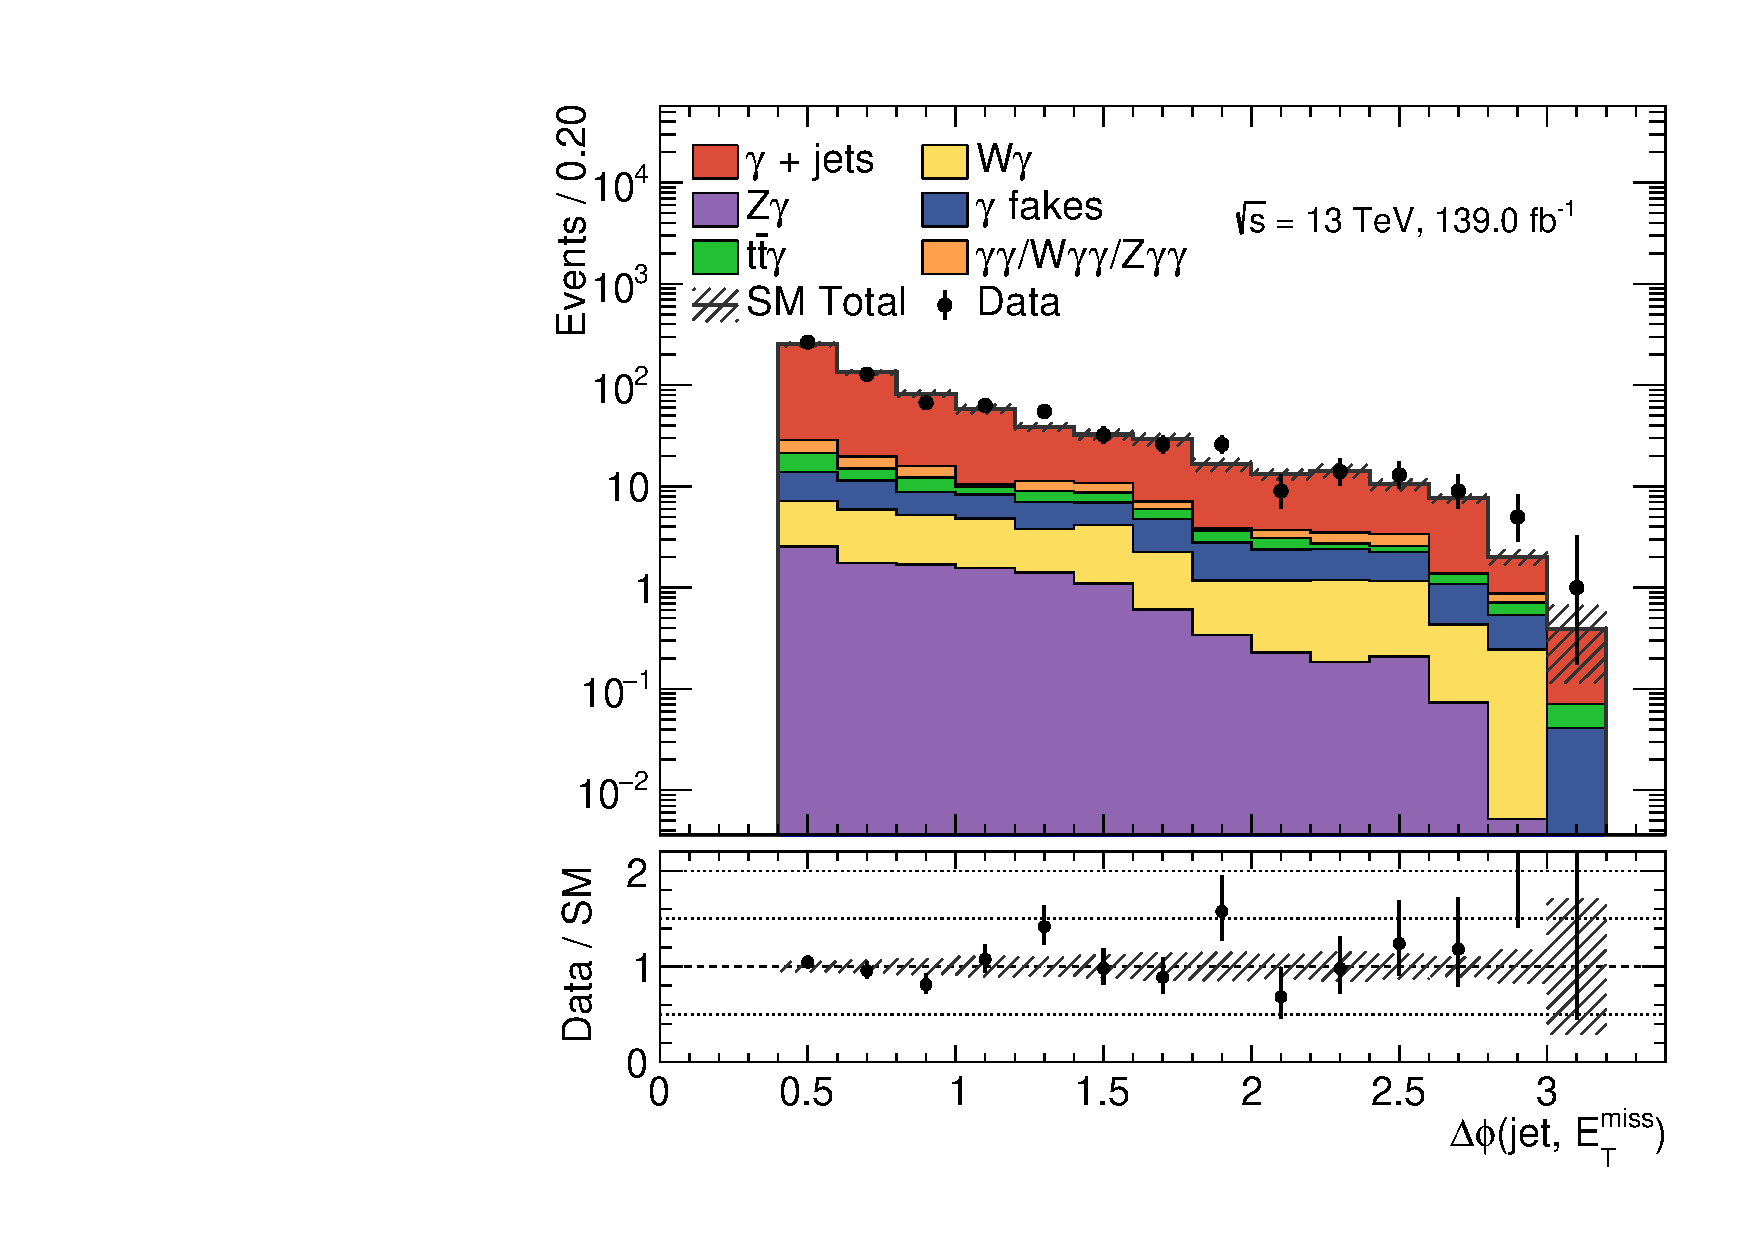
\includegraphics[width=0.32\textwidth]{images/results/fr2_unblind/can_VRQ_dphi_jetmet_afterFit.pdf}

    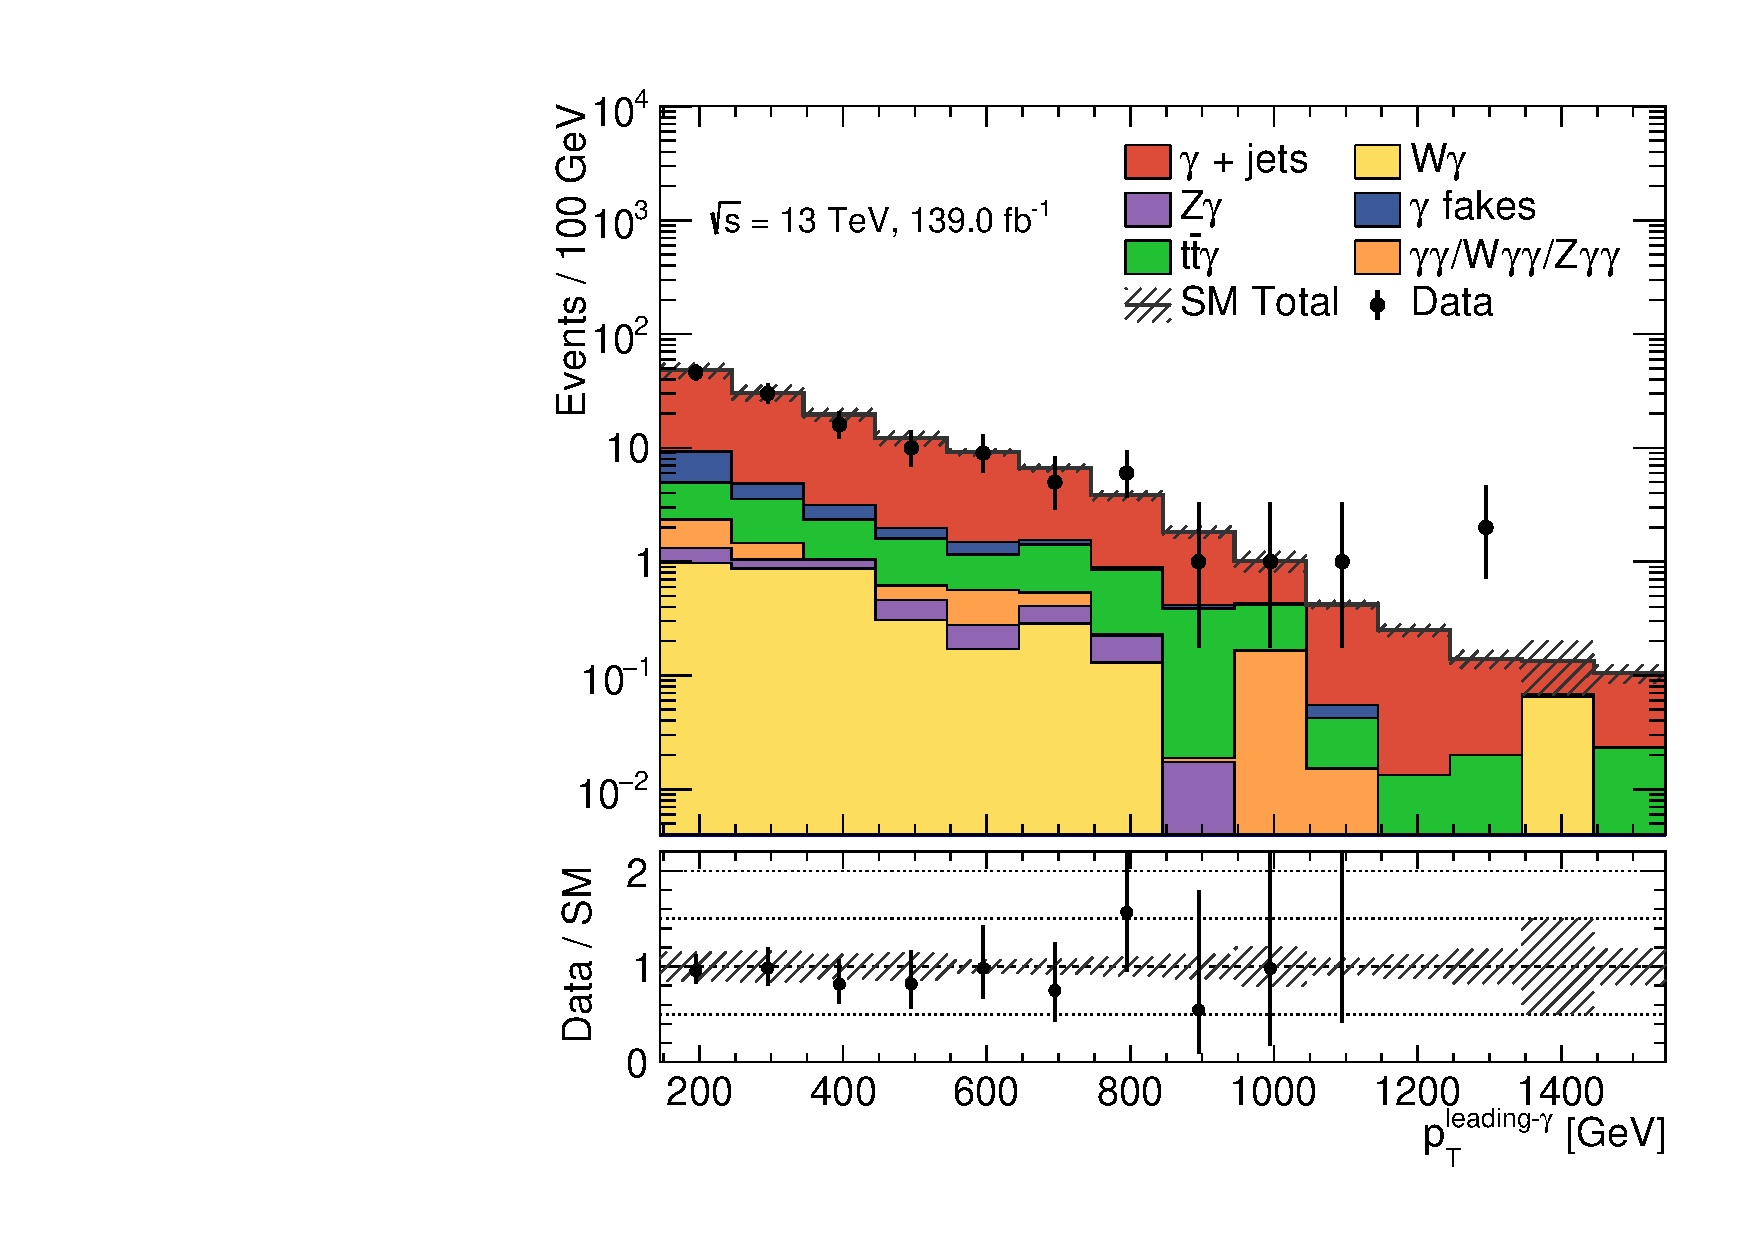
\includegraphics[width=0.32\textwidth]{images/results/fr2_unblind/can_VRM1L_ph_pt0_afterFit.pdf}
    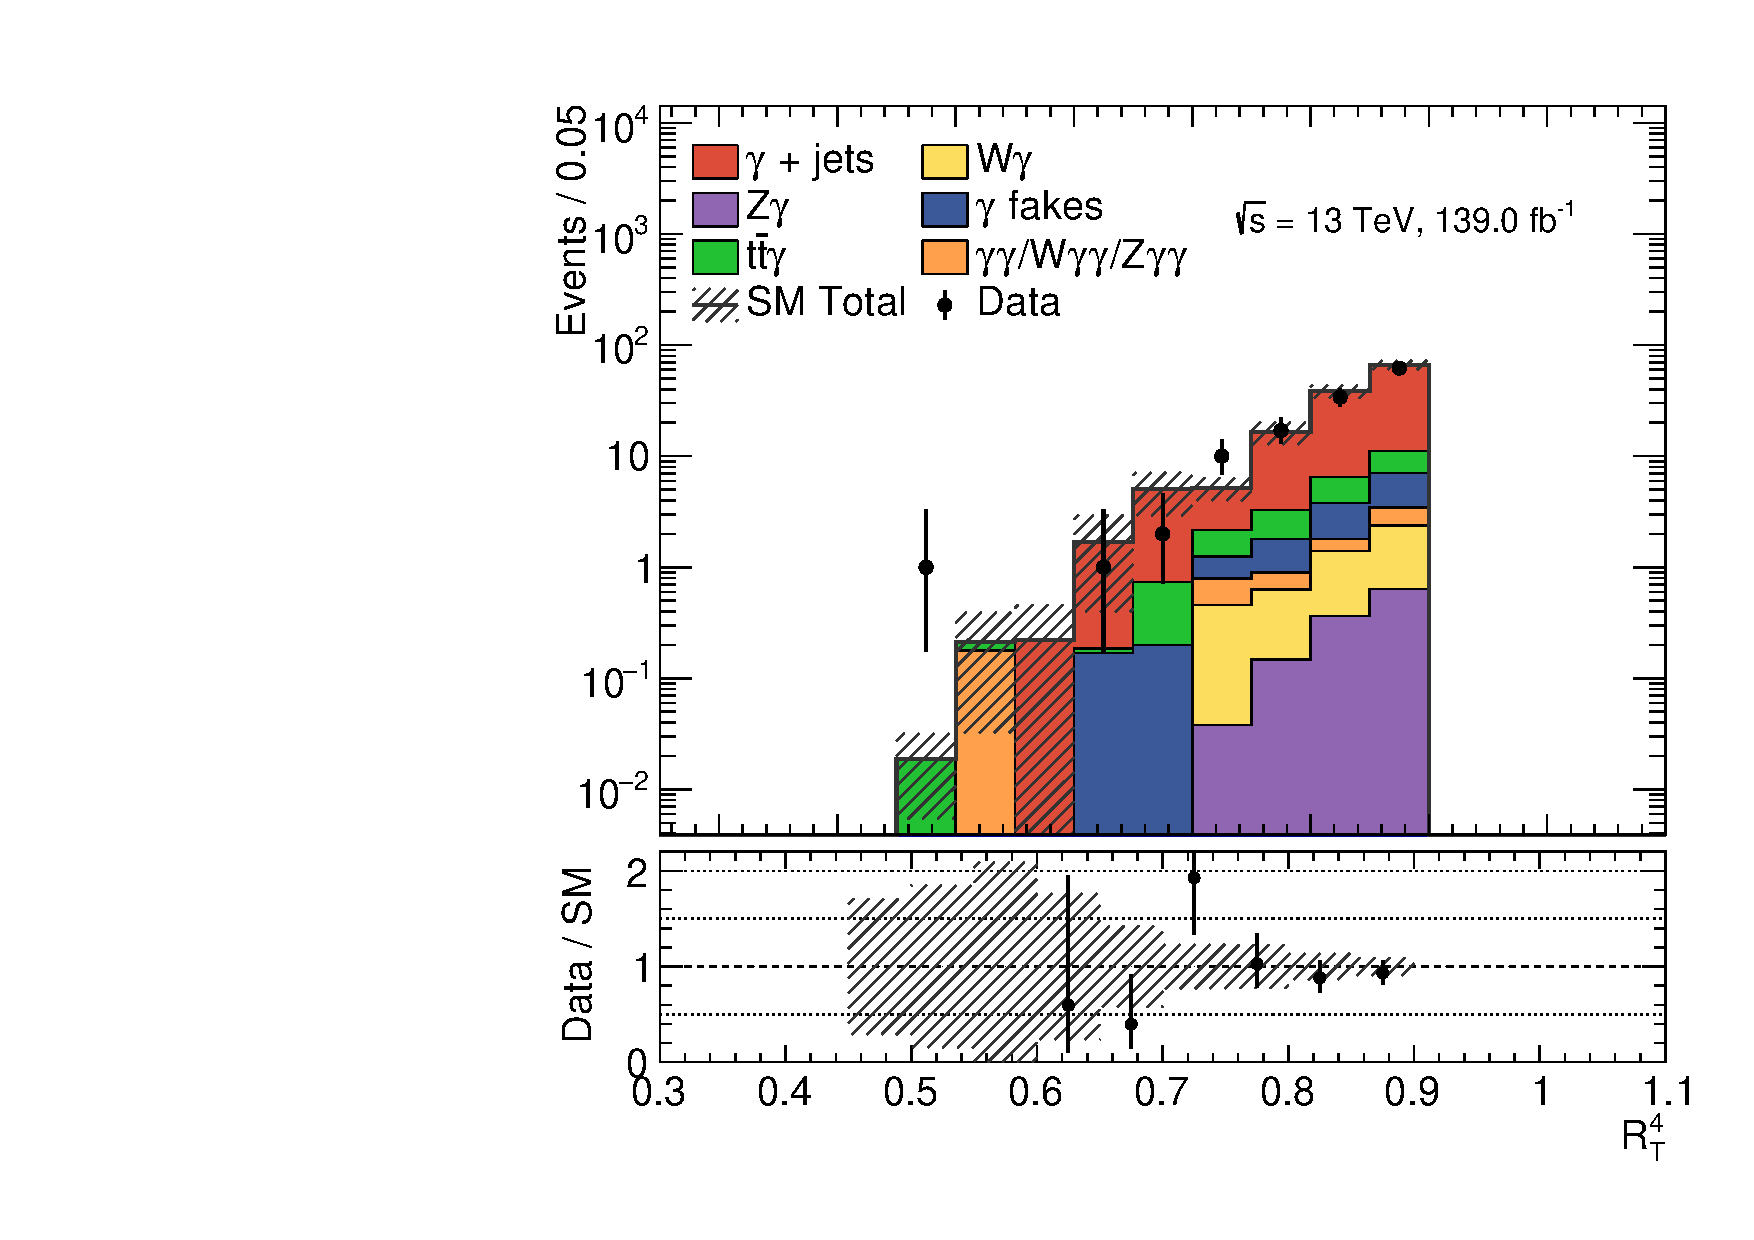
\includegraphics[width=0.32\textwidth]{images/results/fr2_unblind/can_VRM1L_rt4_afterFit.pdf}
    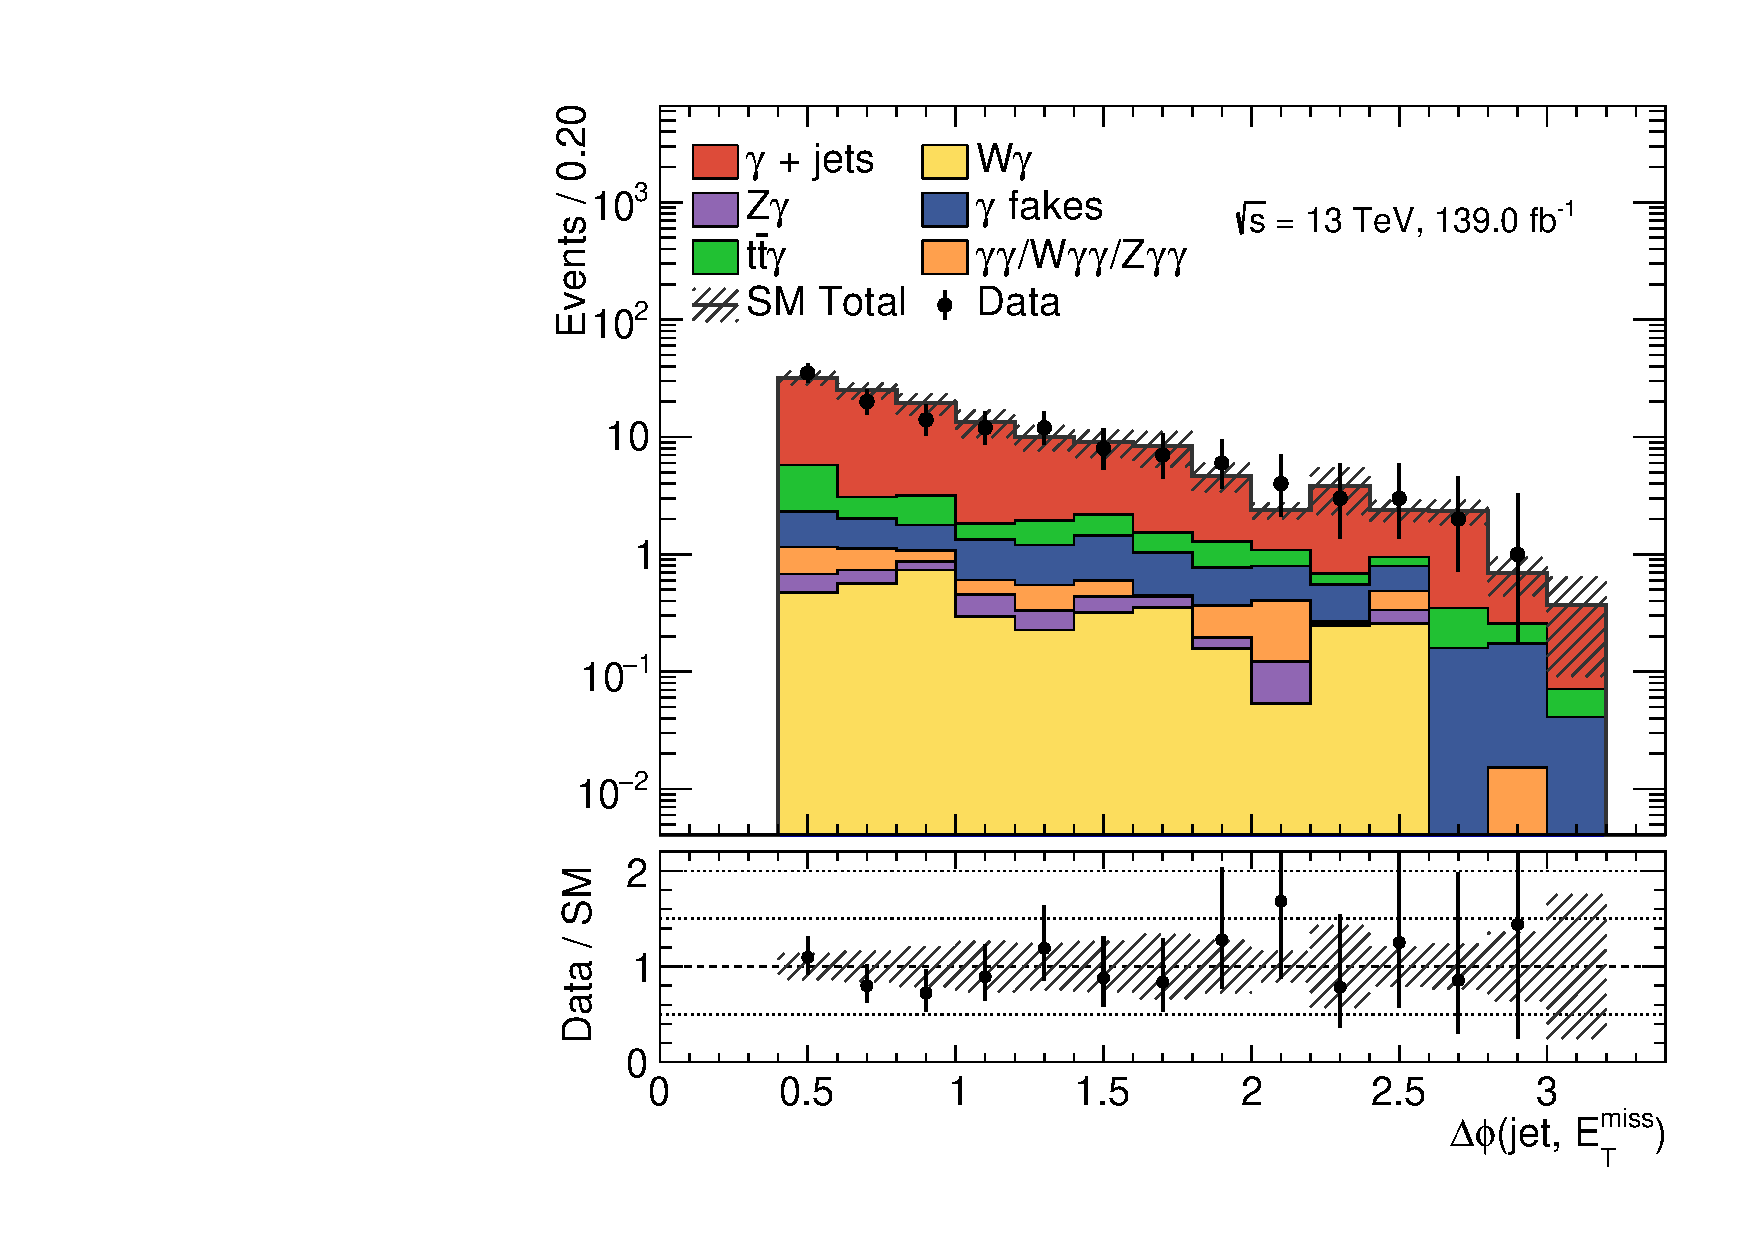
\includegraphics[width=0.32\textwidth]{images/results/fr2_unblind/can_VRM1L_dphi_jetmet_afterFit.pdf}

    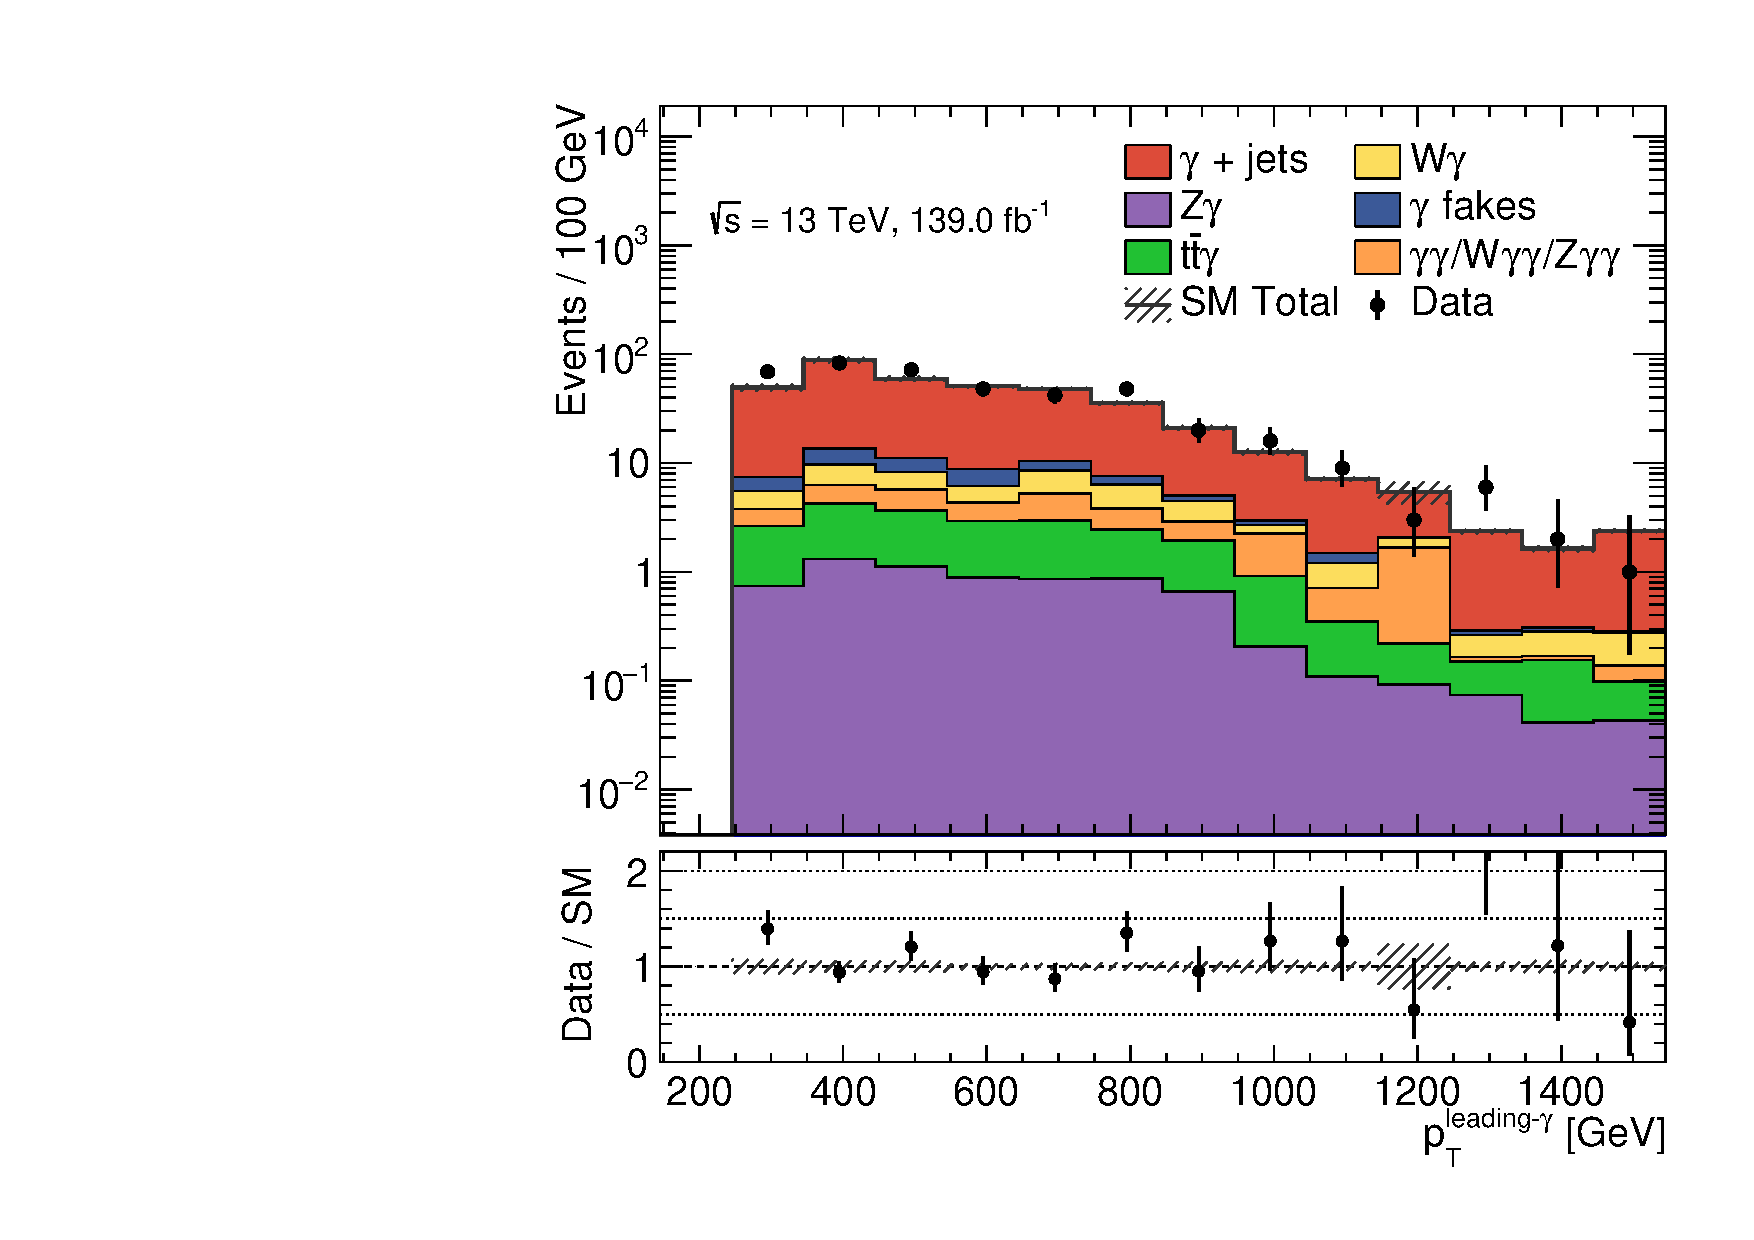
\includegraphics[width=0.32\textwidth]{images/results/fr2_unblind/can_VRM1H_ph_pt0_afterFit.pdf}
    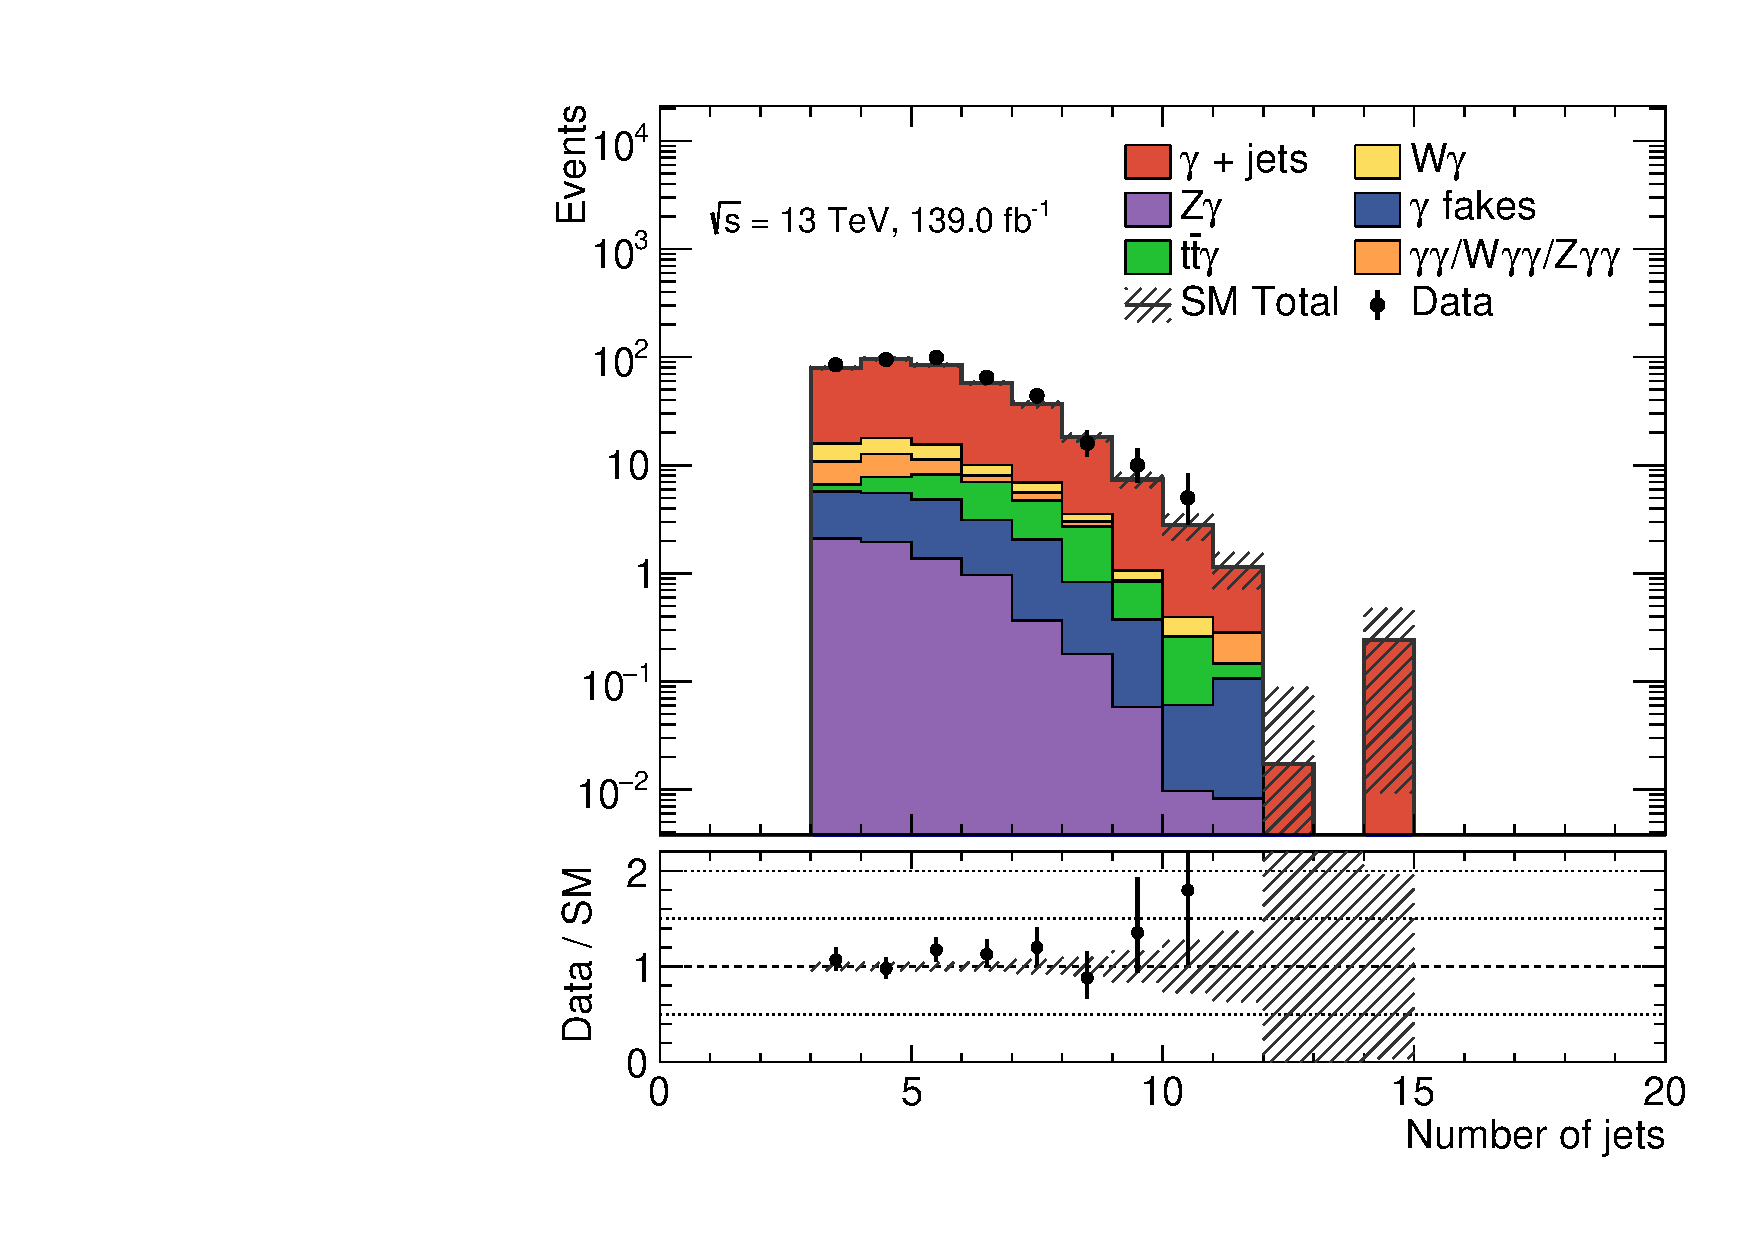
\includegraphics[width=0.32\textwidth]{images/results/fr2_unblind/can_VRM1H_jet_n_afterFit.pdf}
    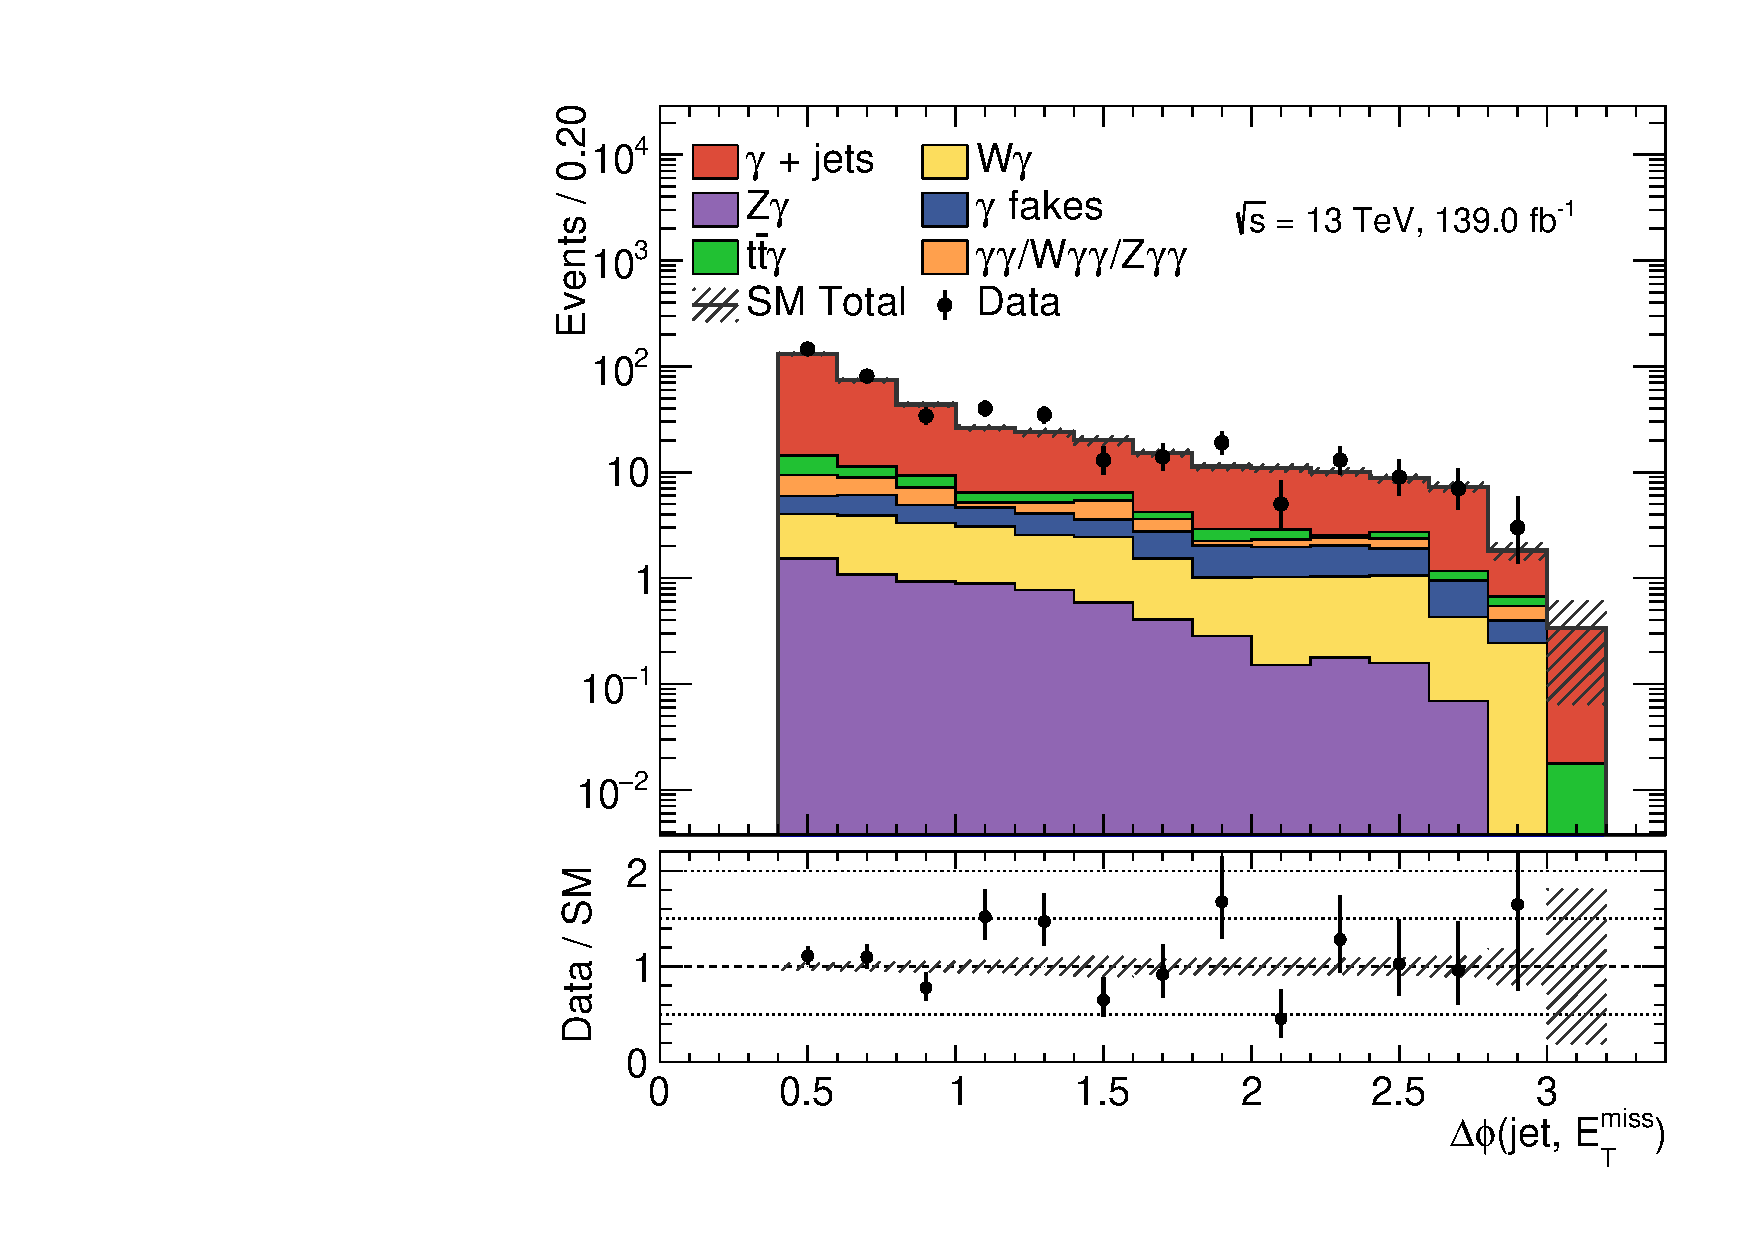
\includegraphics[width=0.32\textwidth]{images/results/fr2_unblind/can_VRM1H_dphi_jetmet_afterFit.pdf}

    
    \caption{Distribuciones de algunas variables significativas en las regiones de validación VRQ (arriba), VRM1H (medio) y VRM1L (abajo) luego del ajuste de solo fondo. Las incertidumbre mostradas son sólo estadísticas.}
    \label{fig:dist_vrqm_bkgonly}
\end{figure}

\begin{figure}[ht!]
  \centering

    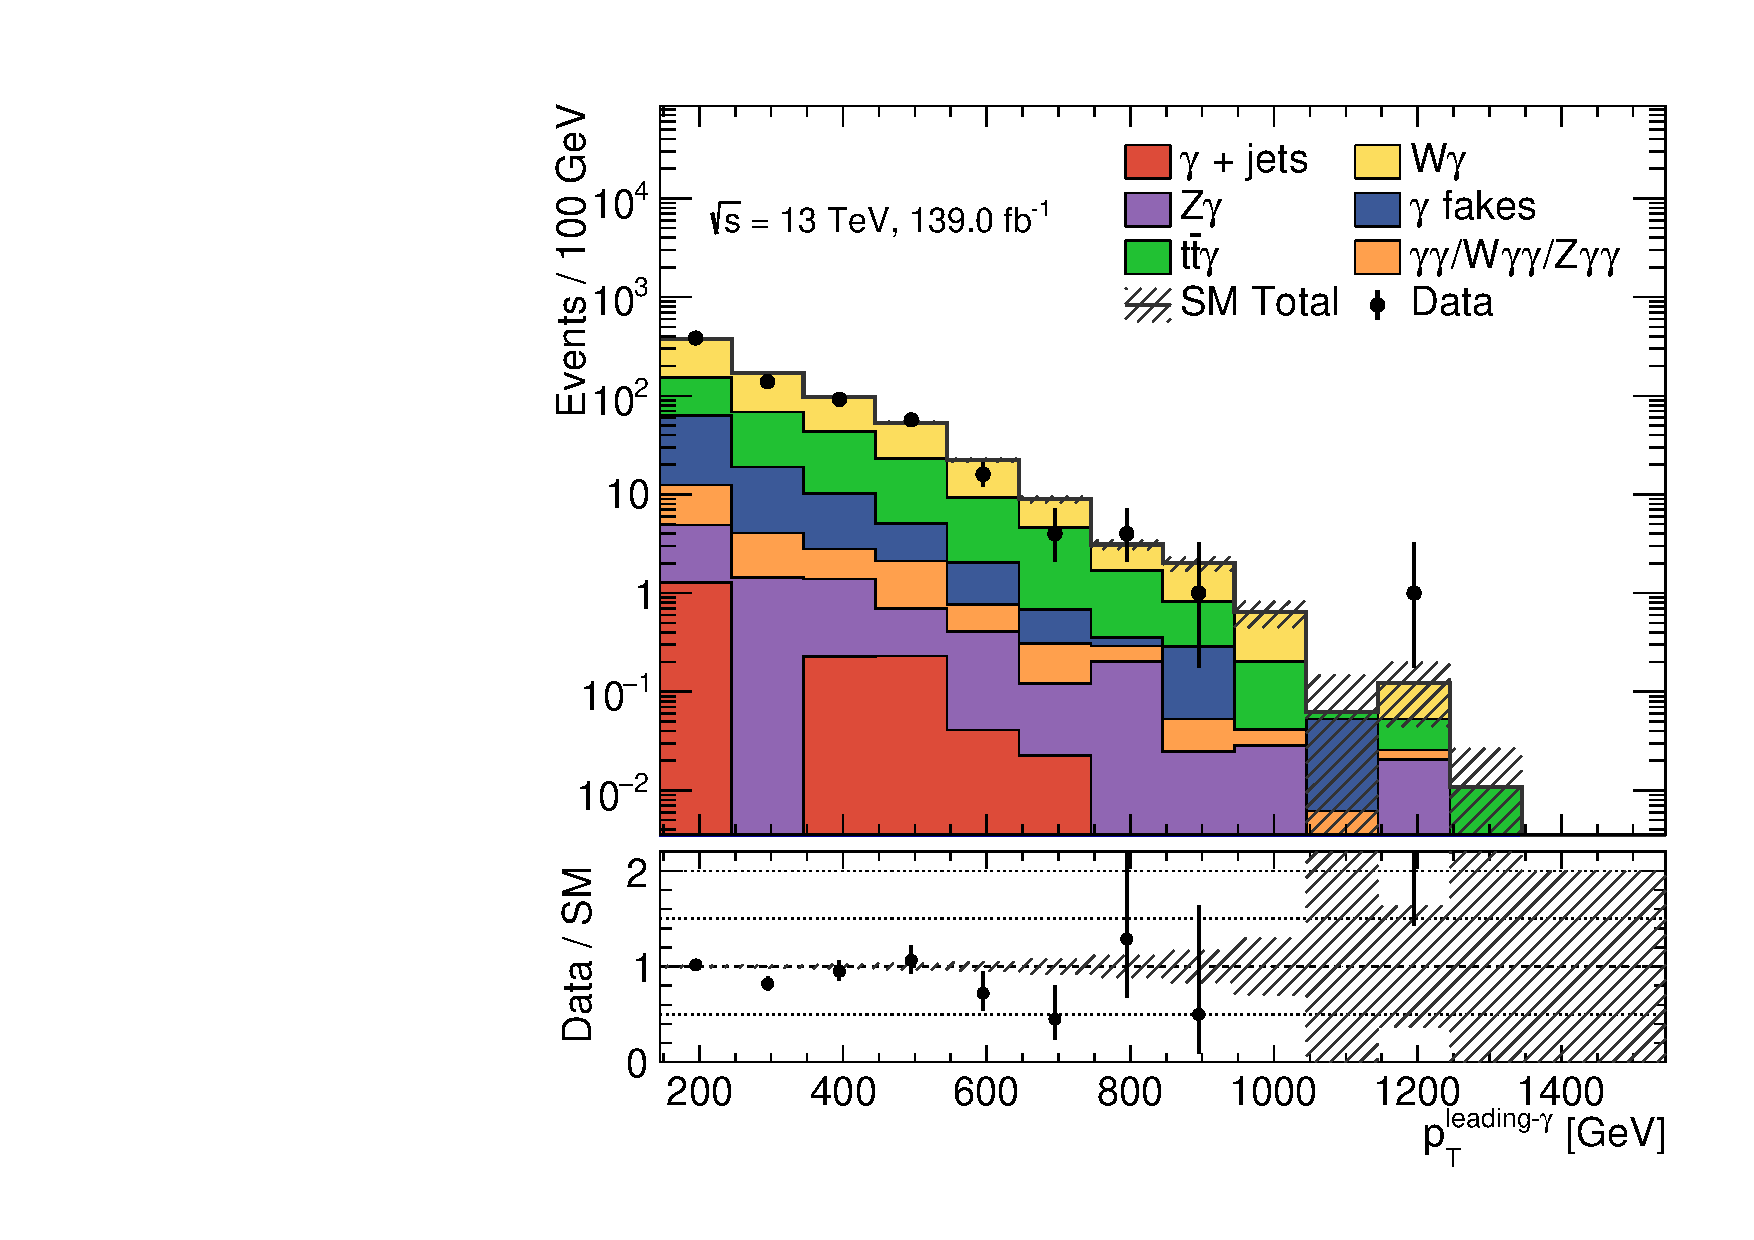
\includegraphics[width=0.32\textwidth]{images/results/fr2_unblind/can_VRL3_ph_pt0_afterFit.pdf}
    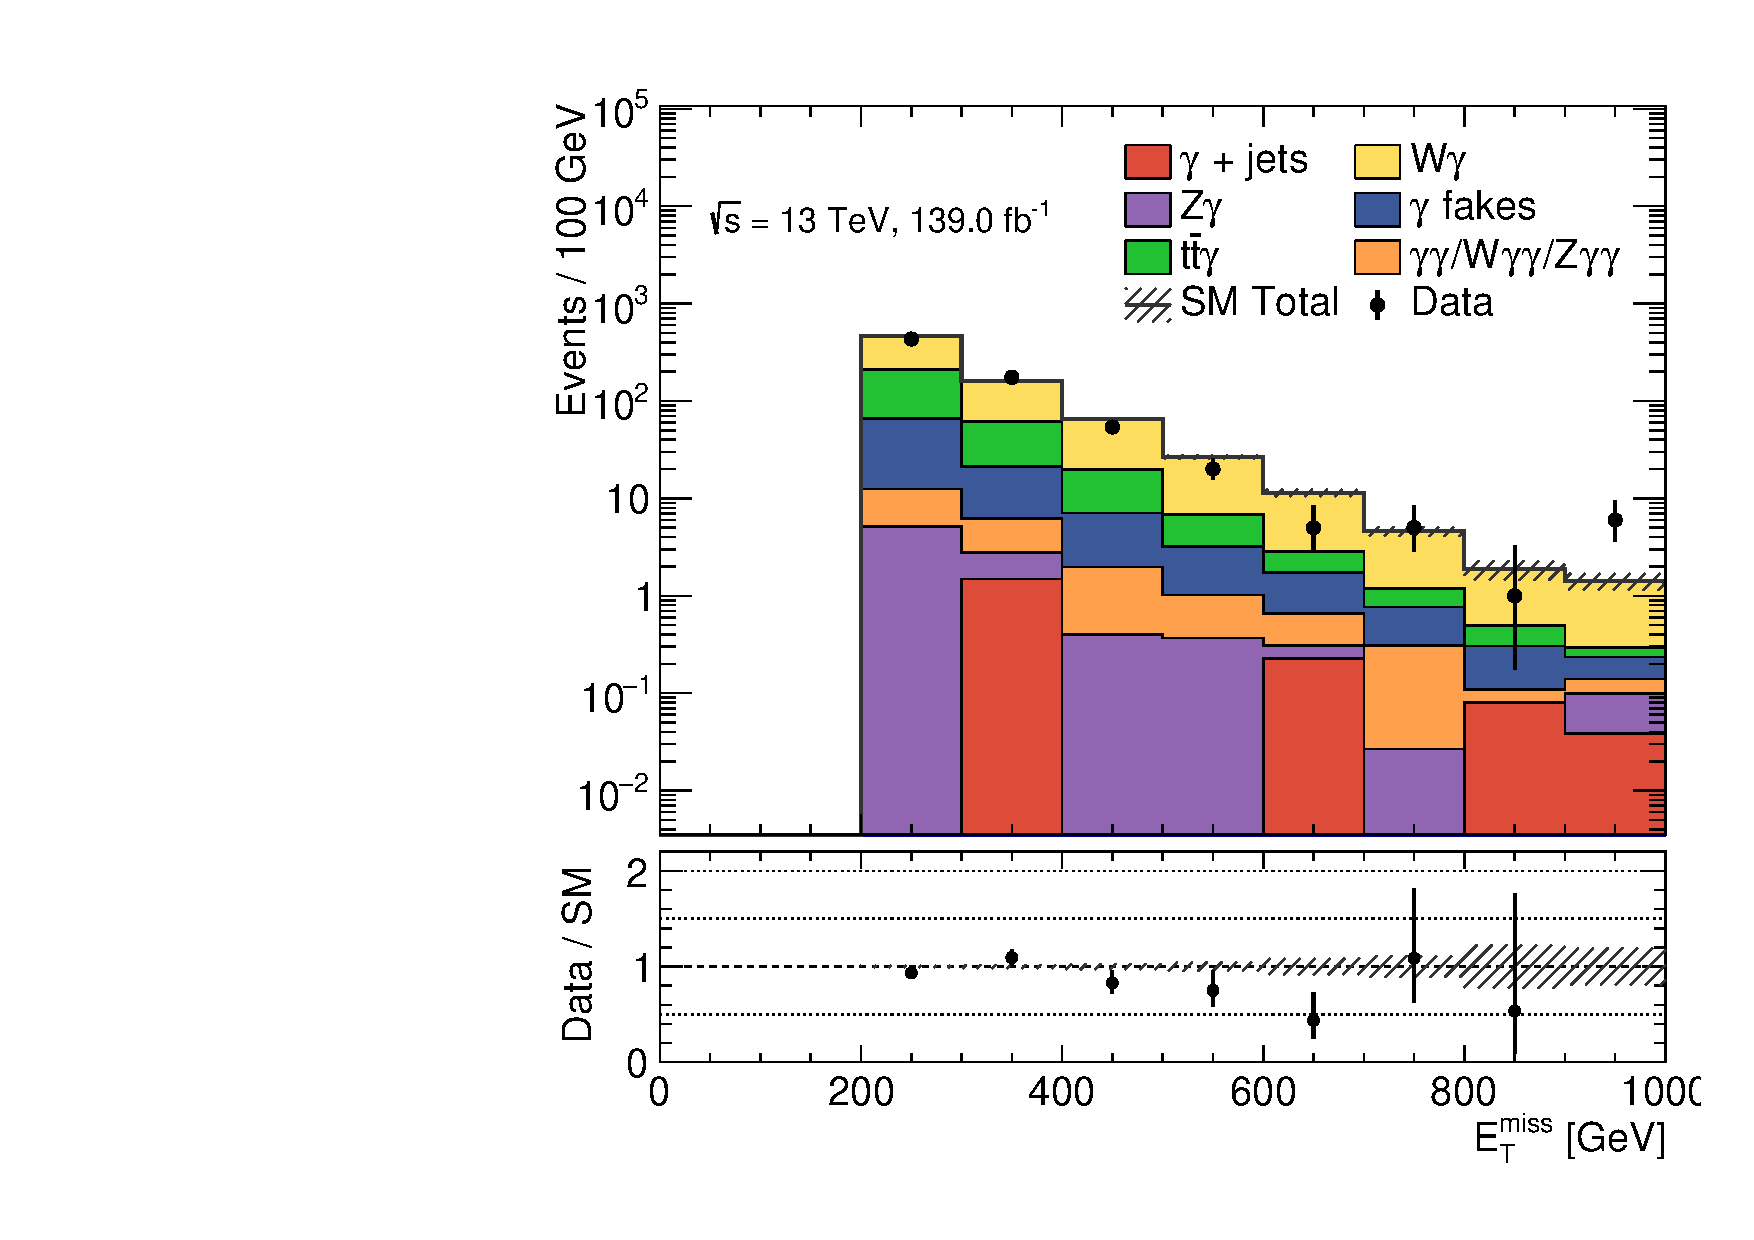
\includegraphics[width=0.32\textwidth]{images/results/fr2_unblind/can_VRL3_met_et_afterFit.pdf}
    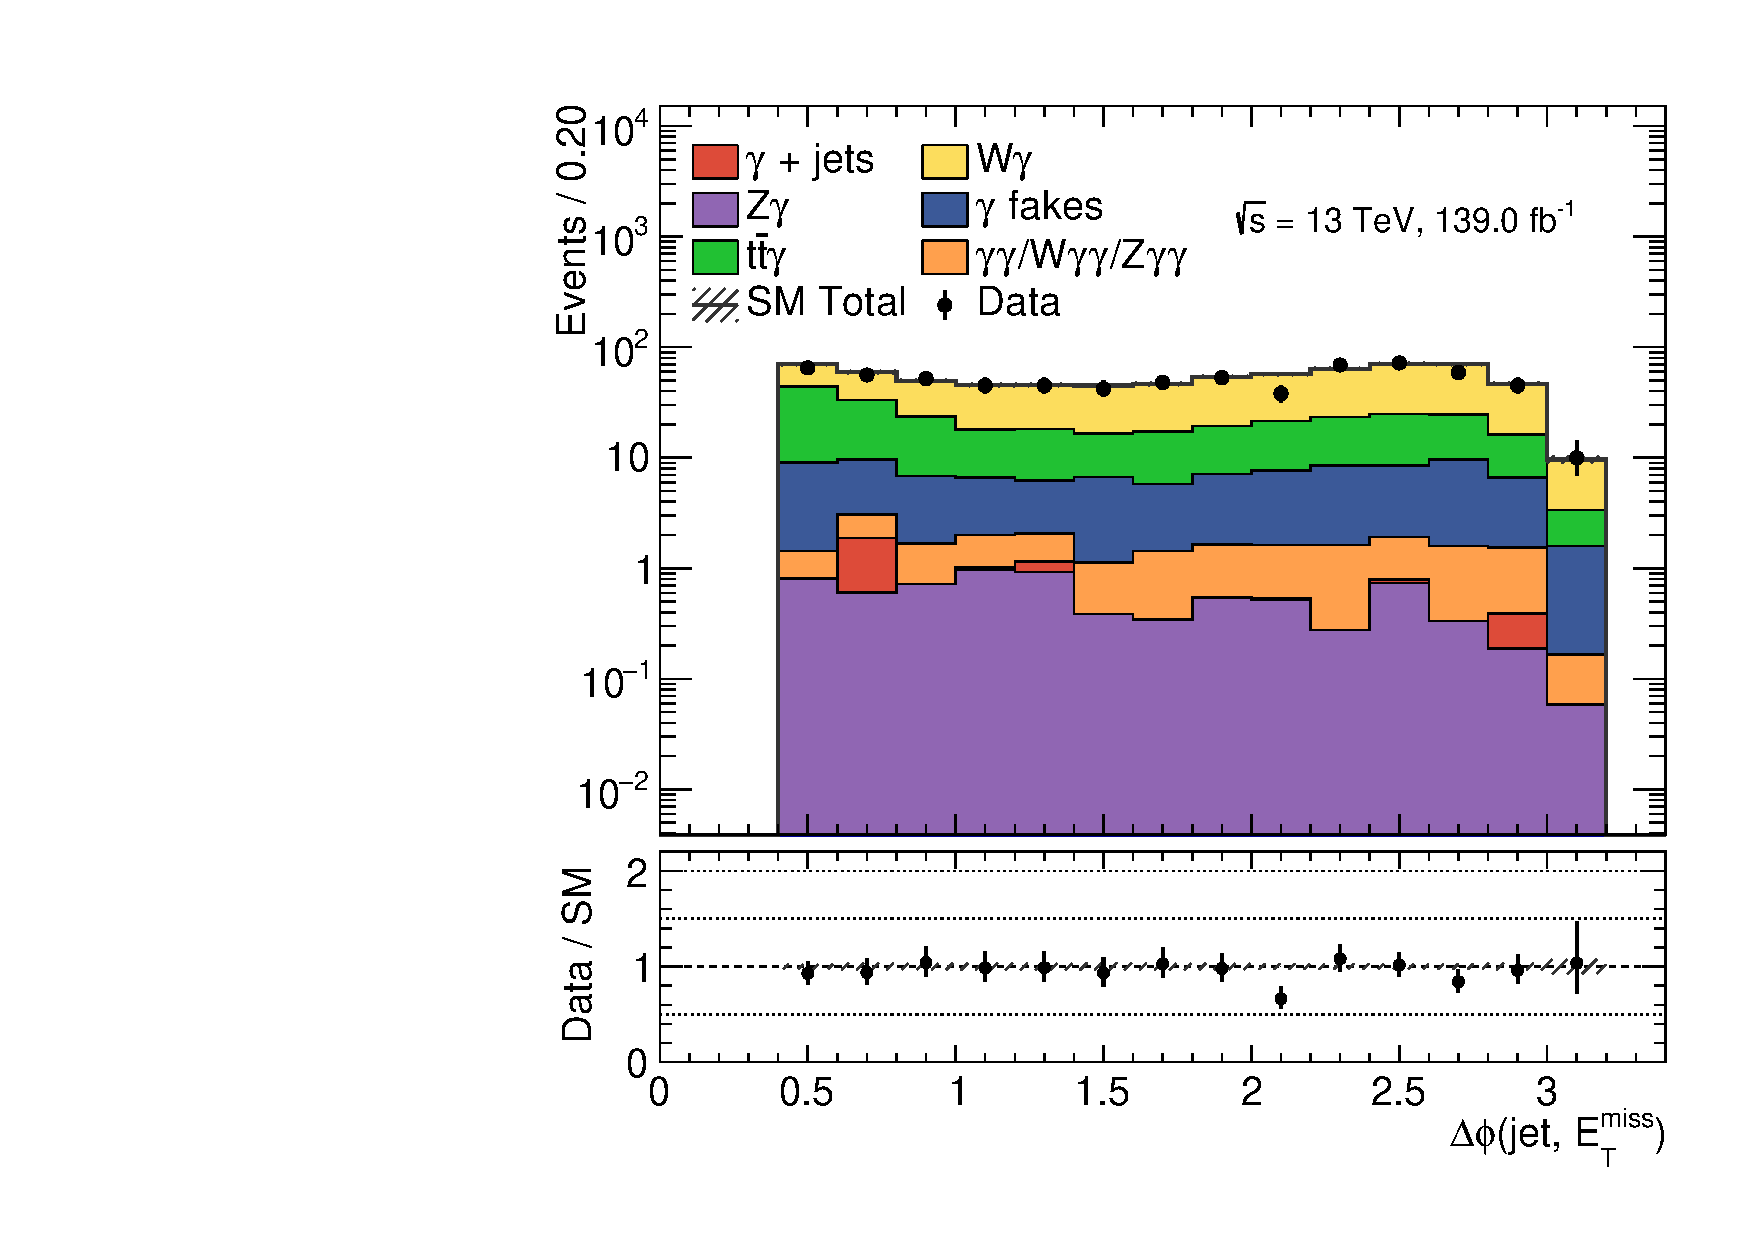
\includegraphics[width=0.32\textwidth]{images/results/fr2_unblind/can_VRL3_dphi_jetmet_afterFit.pdf}

    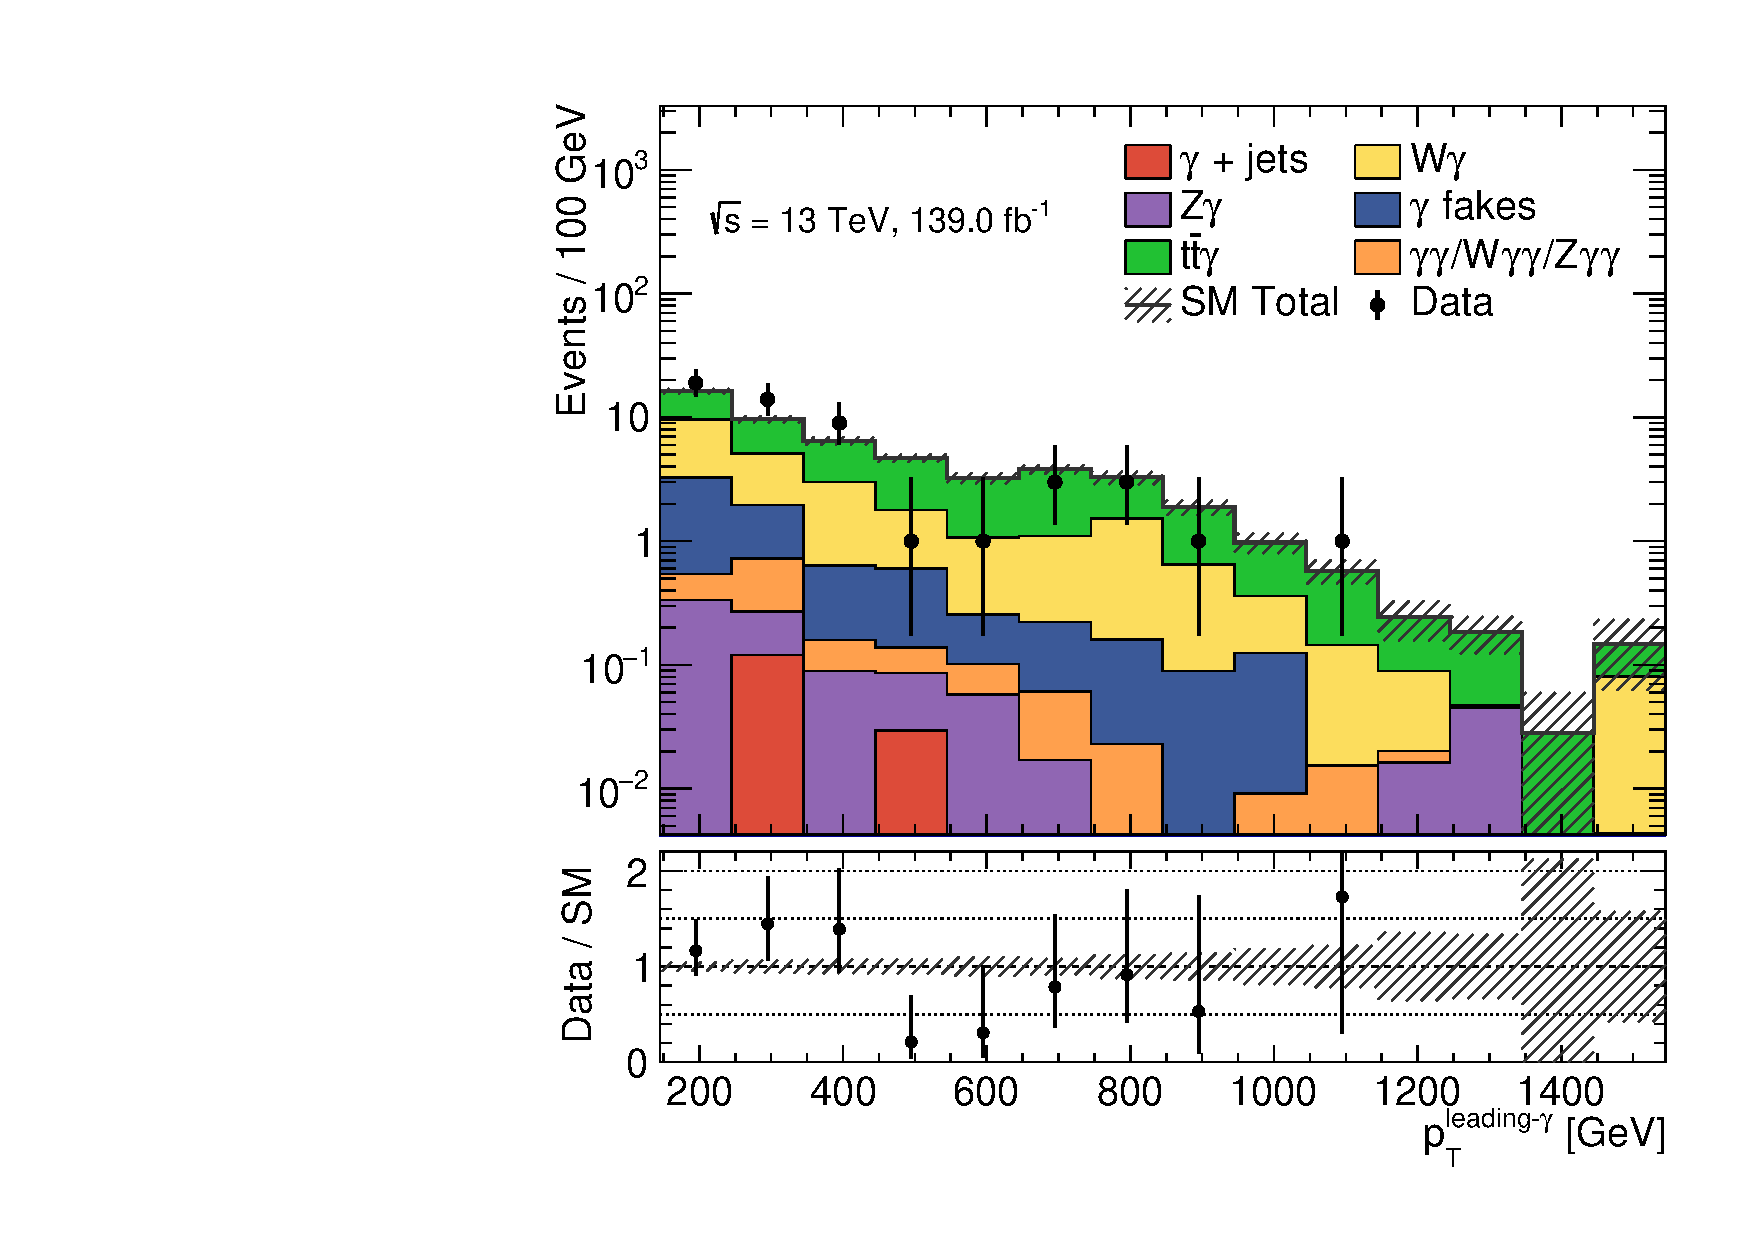
\includegraphics[width=0.32\textwidth]{images/results/fr2_unblind/can_VRL4_ph_pt0_afterFit.pdf}
    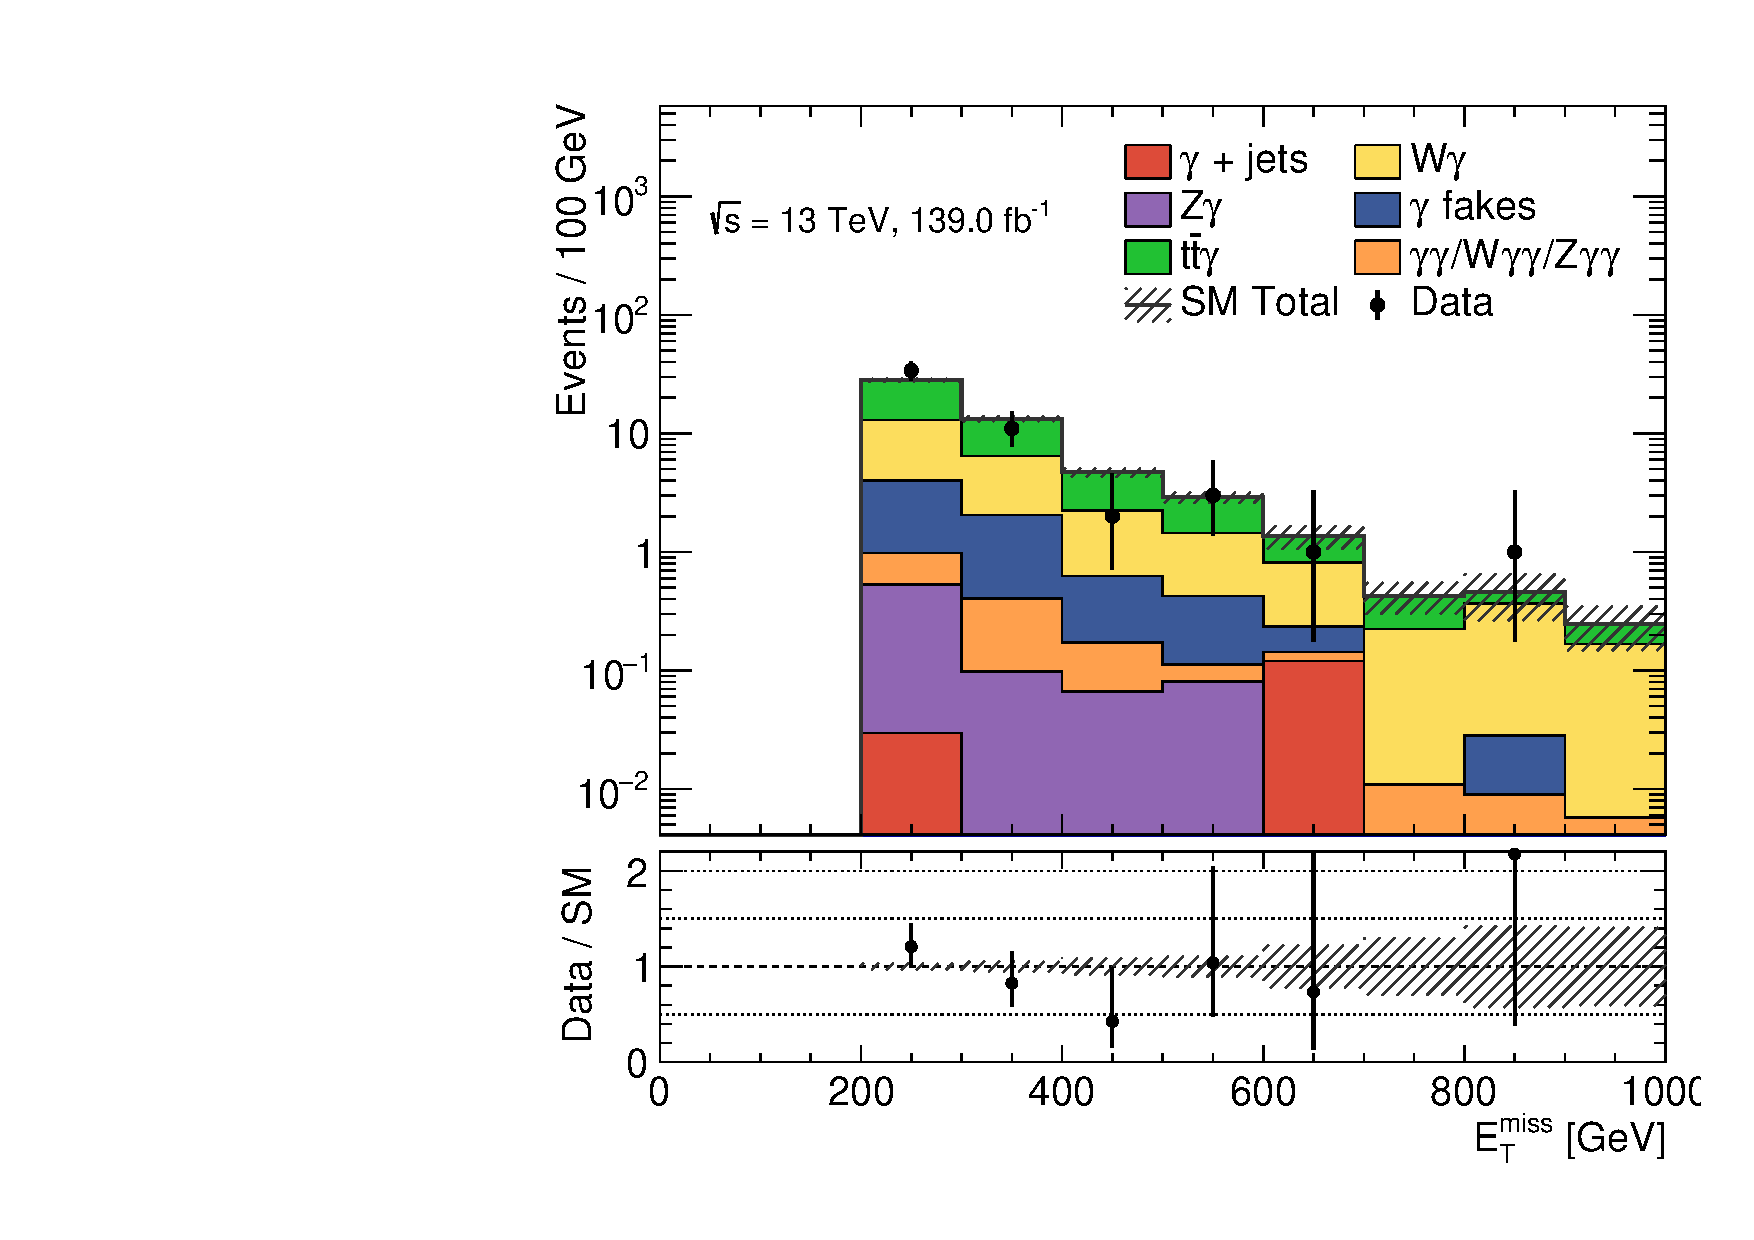
\includegraphics[width=0.32\textwidth]{images/results/fr2_unblind/can_VRL4_met_et_afterFit.pdf}
    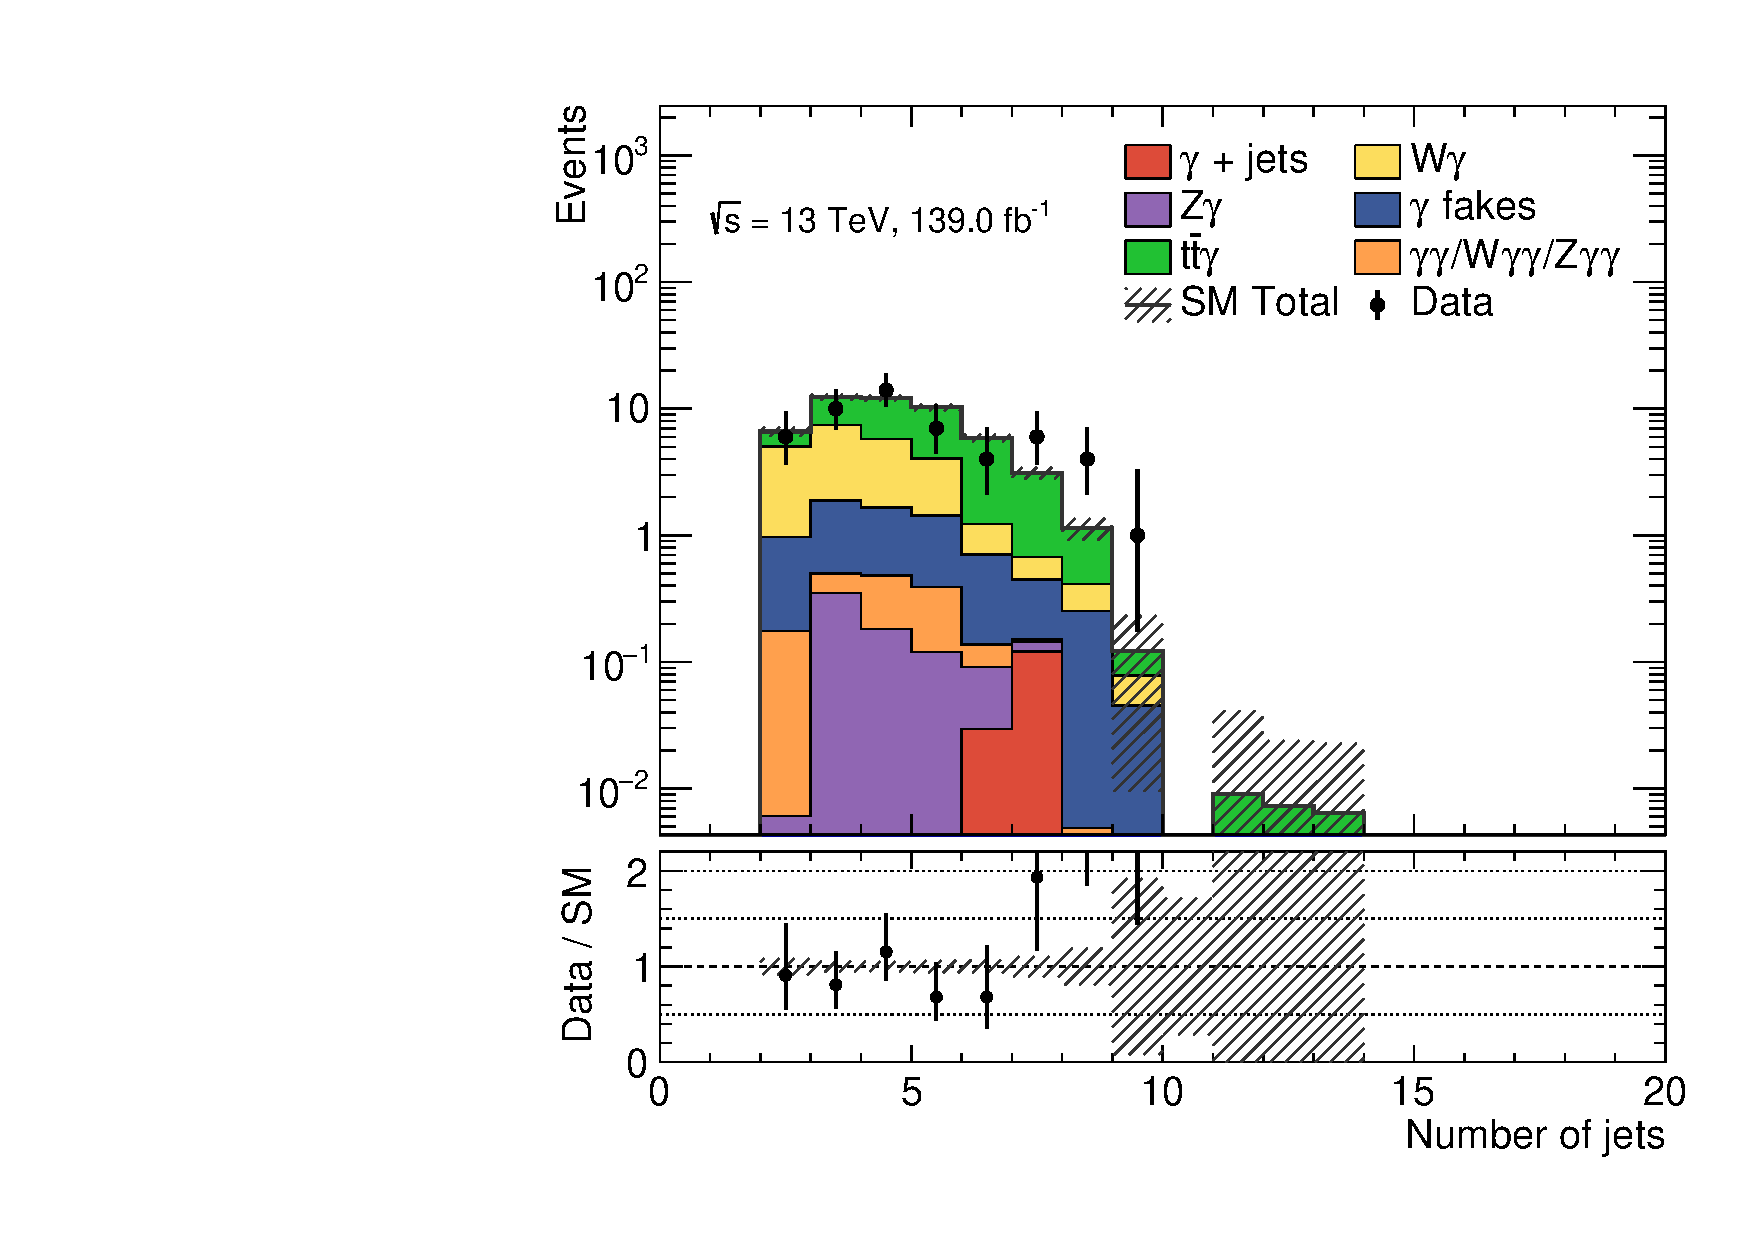
\includegraphics[width=0.32\textwidth]{images/results/fr2_unblind/can_VRL4_jet_n_afterFit.pdf}

    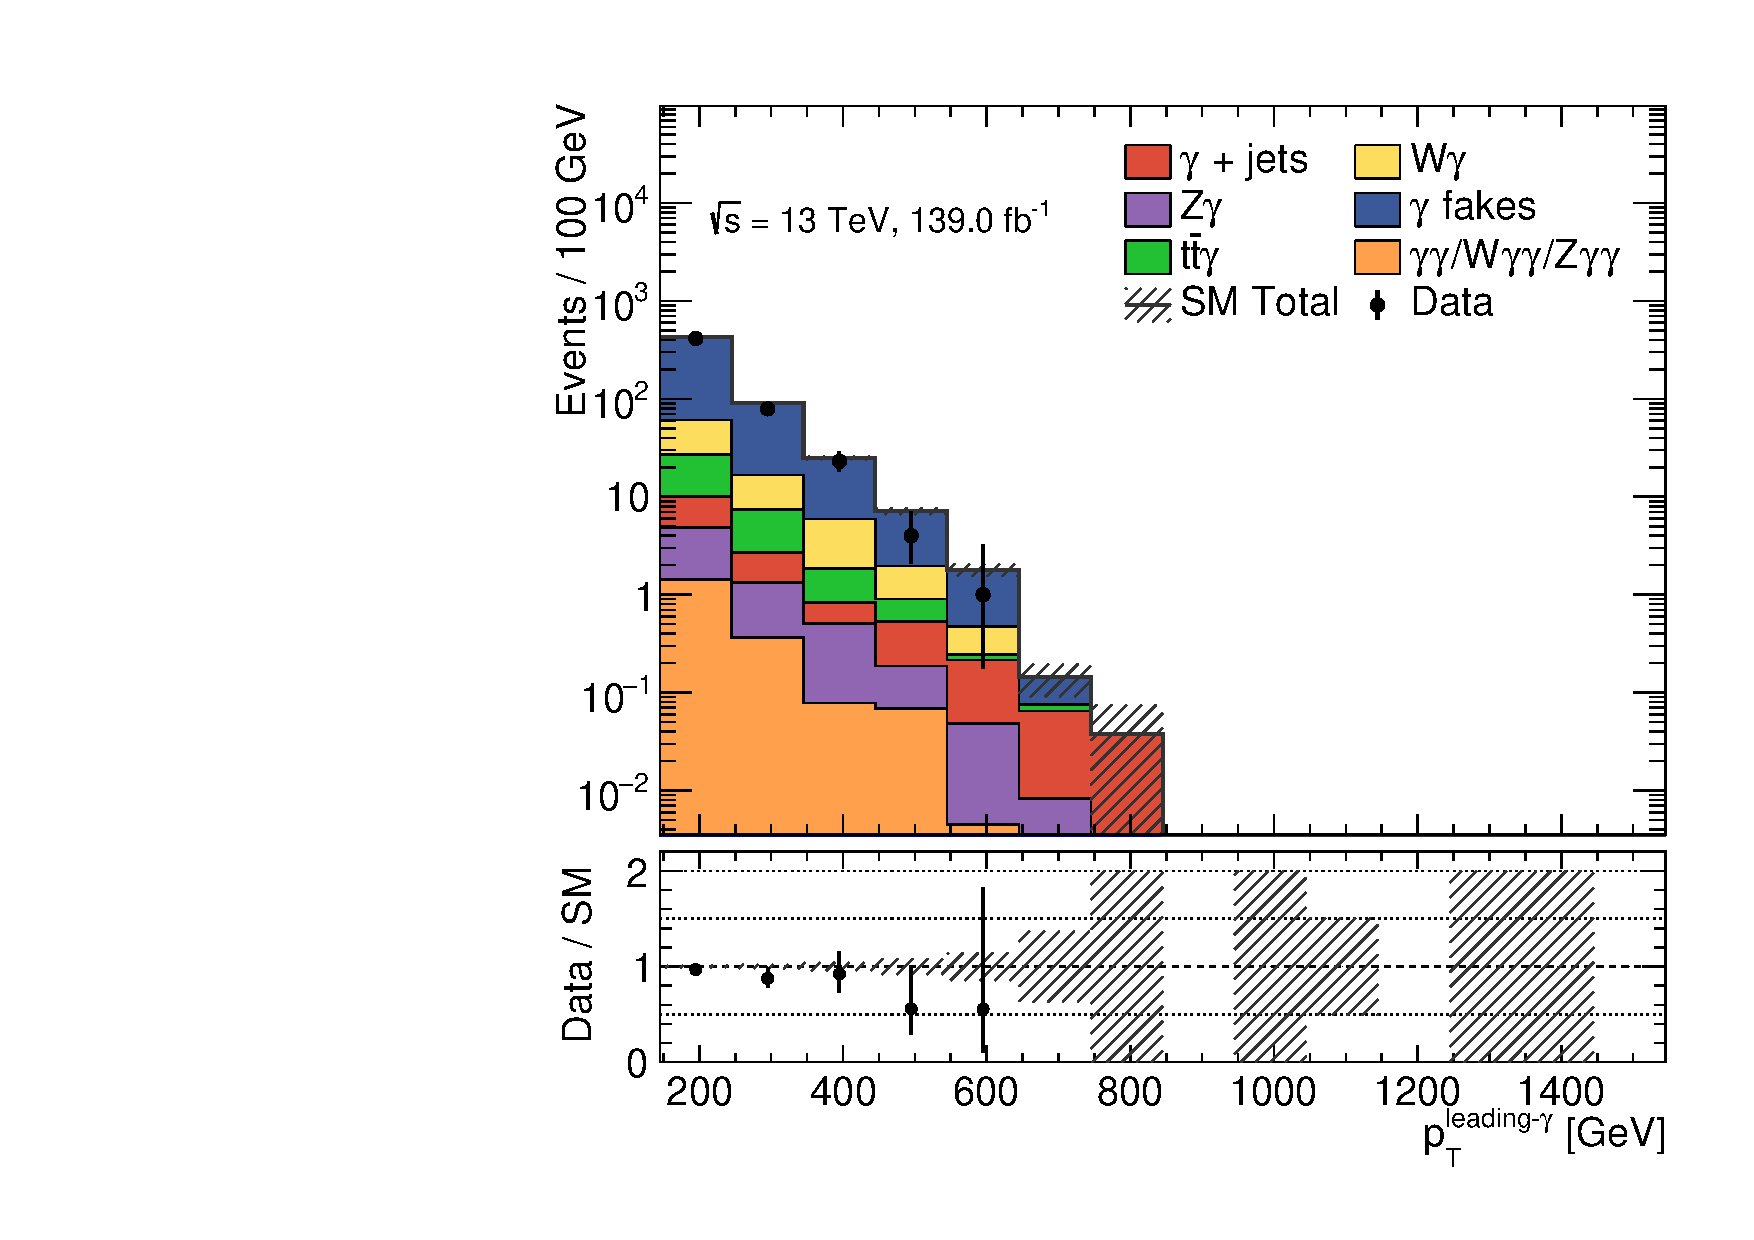
\includegraphics[width=0.32\textwidth]{images/results/fr2_unblind/can_VRE_ph_pt0_afterFit.pdf}
    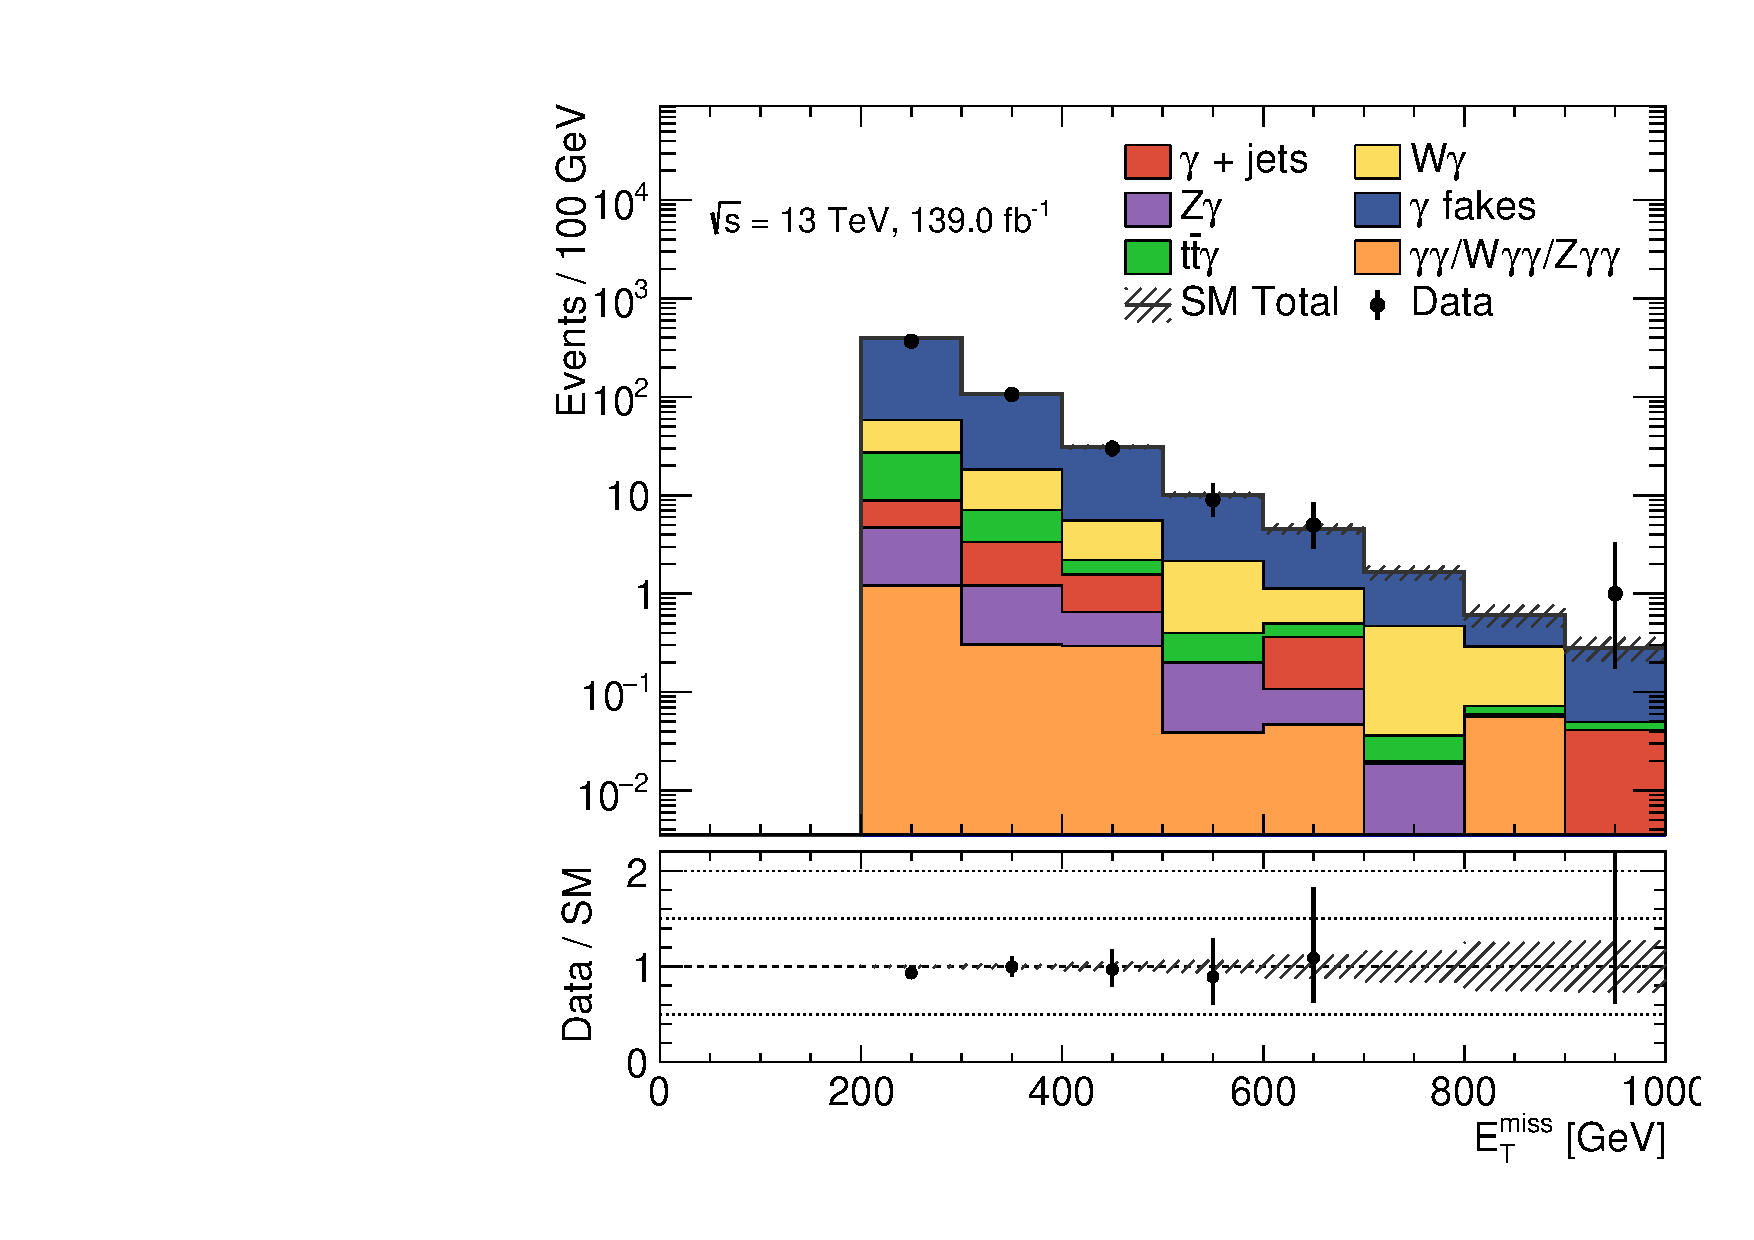
\includegraphics[width=0.32\textwidth]{images/results/fr2_unblind/can_VRE_met_et_afterFit.pdf}
    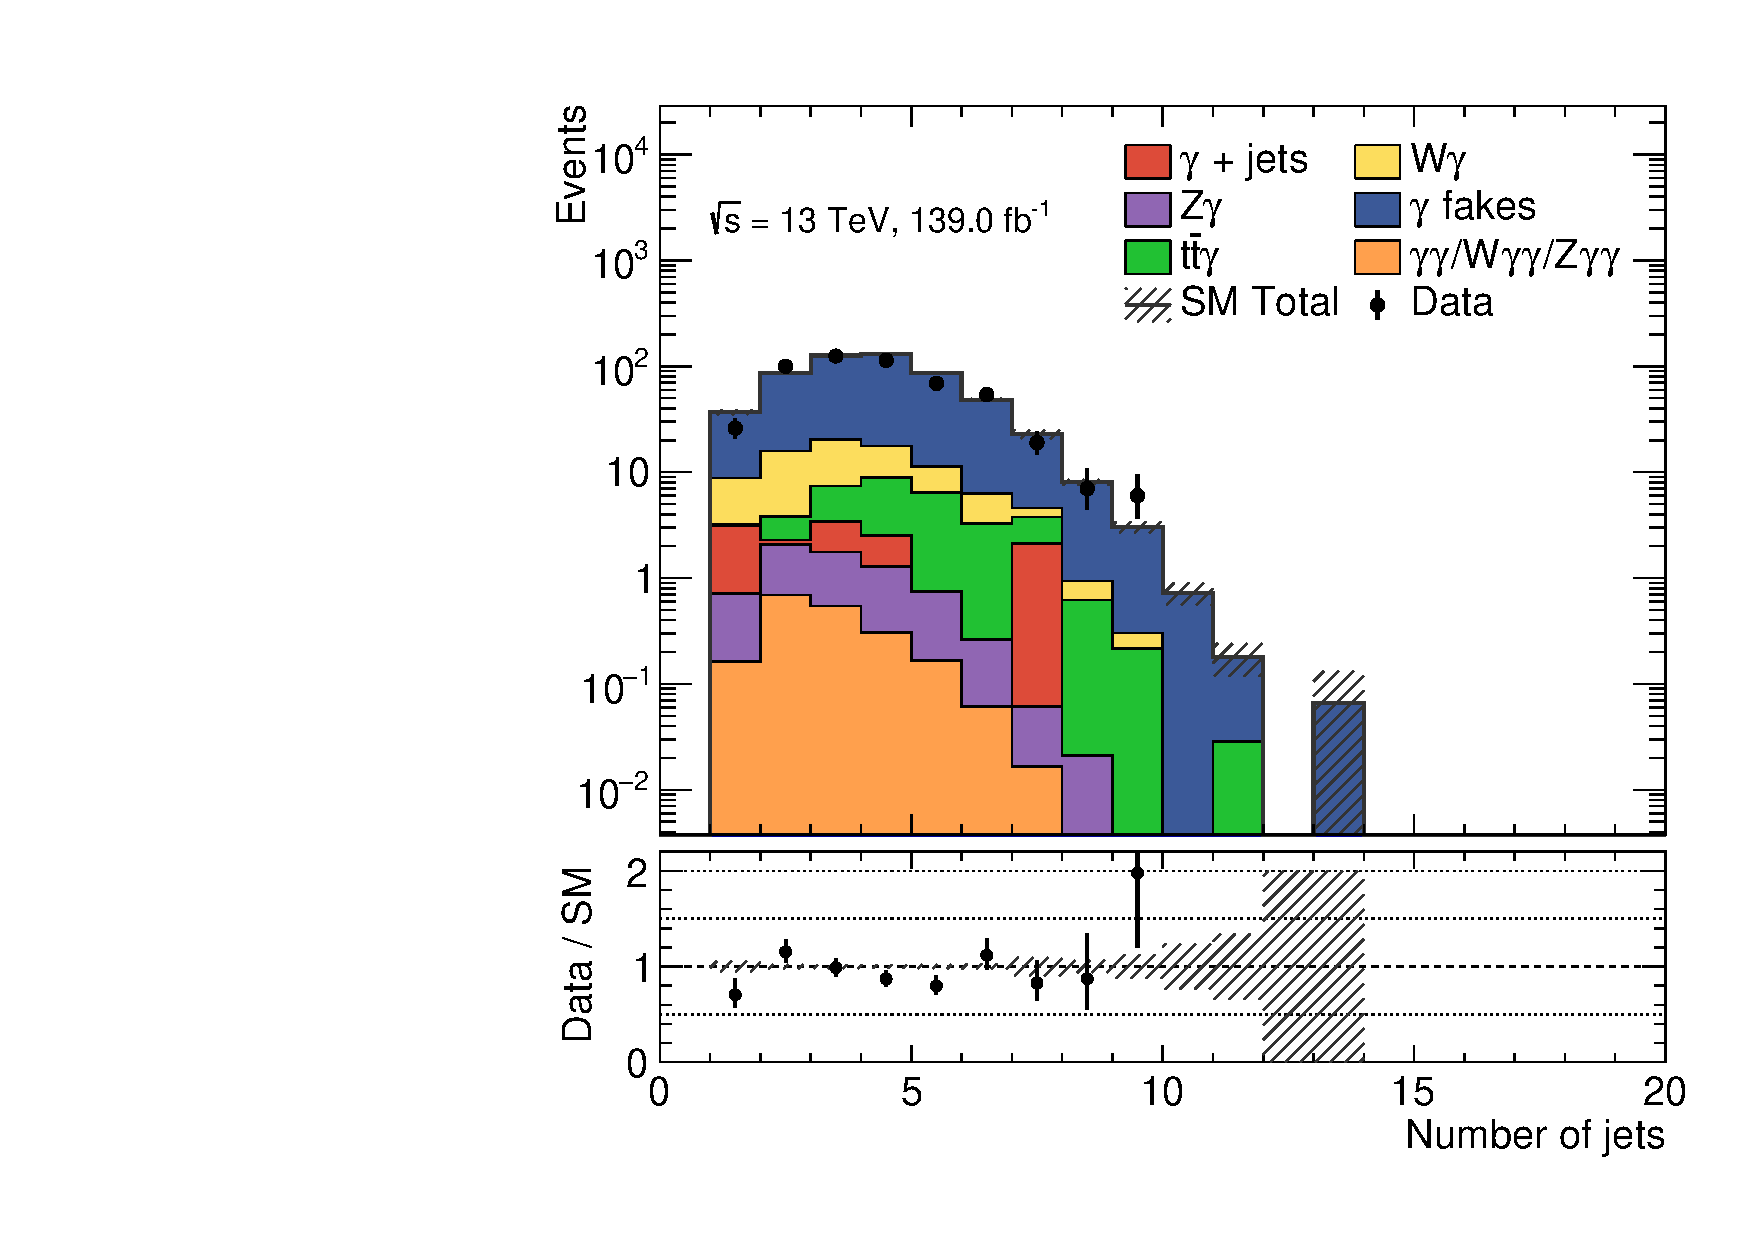
\includegraphics[width=0.32\textwidth]{images/results/fr2_unblind/can_VRE_jet_n_afterFit.pdf}

    
    \caption{Distribuciones de algunas variables significativas en las regiones de validación VRL3 (arriba), VRL4 (medio) y VRE (abajo) luego del ajuste de solo fondo. Las incertidumbre mostradas son sólo estadísticas.}
    \label{fig:dist_vrle_bkgonly}
\end{figure}


% \solved{Cosas que no estoy poniendo: signal contamination en las VRs, correlacion parametros del ajuste, tabla de incertezas sistematicas, pull de los NPs} solo tabla de sistematicos




\subsection{Resultados en las regiones de señal}

Luego de la estimación de los fondos en las regiones de señal y su correcta validación en sus respectivas VRs, se procedió a la observación de los datos en dichas regiones. En la Tabla \ref{tab:fit_result_sr_unblinded} se muestra el número de eventos observados y la estimación de los fondos en cada región de señal. El número total de eventos observados para la SRL es de $2$, para la SRM de $0$ y para la SRH de $5$, mientras que el número de eventos esperados es de $2.67\pm0.75$, $2.55\pm0.64$ y $2.55\pm0.44$ respectivamente. A su vez, en la Figura \ref{fig:regions_pulls_unblinded} se observa el resumen de la estimación de fondo y datos observados para cada región del análisis. En la Figura \ref{fig:met_n-1_SRL_SRM_SRH_fr2} se observa la distribución de \met para las tres regiones de señal, pero omitiendo el corte en esa variable de las mismas (gráfico N-1), donde se incluye las estimaciones de los fondos, la de los datos observados y la señal. En la Tabla \ref{tab:syst_rel_impact} se muestra el aporte porcentual de cada sistemático en las regiones de señal, siendo predominantes las asociadas a la escala de energía de los jets y las incertezas teóricas.


\begin{table}[ht!]
  \centering
  \caption{Número de datos observados y estimación de fondo en las regiones de señal, para una luminosidad de $139.0\ \ifb$.}
  \begin{tabular}{lrrr}
\hline
Signal Regions & SRL & SRM & SRH \\
\hline
Observed events & 2 & 0 & 5 \\
\hline
Expected SM events & $2.67 \pm 0.75$ & $2.55 \pm 0.64$ & $2.55 \pm 0.44$ \\
\hline
$e\rightarrow\gamma$ fakes & $0.22 \pm 0.08$ & $0.04 \pm 0.03$ & $0.06 \pm 0.04$ \\
$j\rightarrow\gamma$ fakes & $0.15 \pm 0.09$ & $0.14 \pm 0.09$ & $0.09 \pm 0.07$ \\
$\gamma$ + jets & $0.49 \pm 0.29$ & $0.17 \pm 0.10$ & $0.07 \pm 0.01$ \\
$W\gamma$ & $0.55 \pm 0.37$ & $0.70 \pm 0.42$ & $1.08 \pm 0.21$ \\
$Z(\rightarrow\ell\ell)\gamma$ & $0.03_{-0.03}^{+0.03}$ & $0.03 \pm 0.01$ & $0.00 \pm 0.00$ \\
$Z(\rightarrow\nu\nu)\gamma$ & $0.31 \pm 0.11$ & $0.35 \pm 0.12$ & $0.94 \pm 0.28$ \\
$t\bar{t}\gamma$ & $0.70 \pm 0.18$ & $0.87 \pm 0.18$ & $0.22 \pm 0.05$ \\
$\gamma\gamma / W\gamma\gamma / Z\gamma\gamma$ & $0.23 \pm 0.11$ & $0.25 \pm 0.10$ & $0.08 \pm 0.01$ \\
\hline
\end{tabular}

  \label{tab:fit_result_sr_unblinded}
\end{table}

\begin{figure}[ht!]
  \centering
  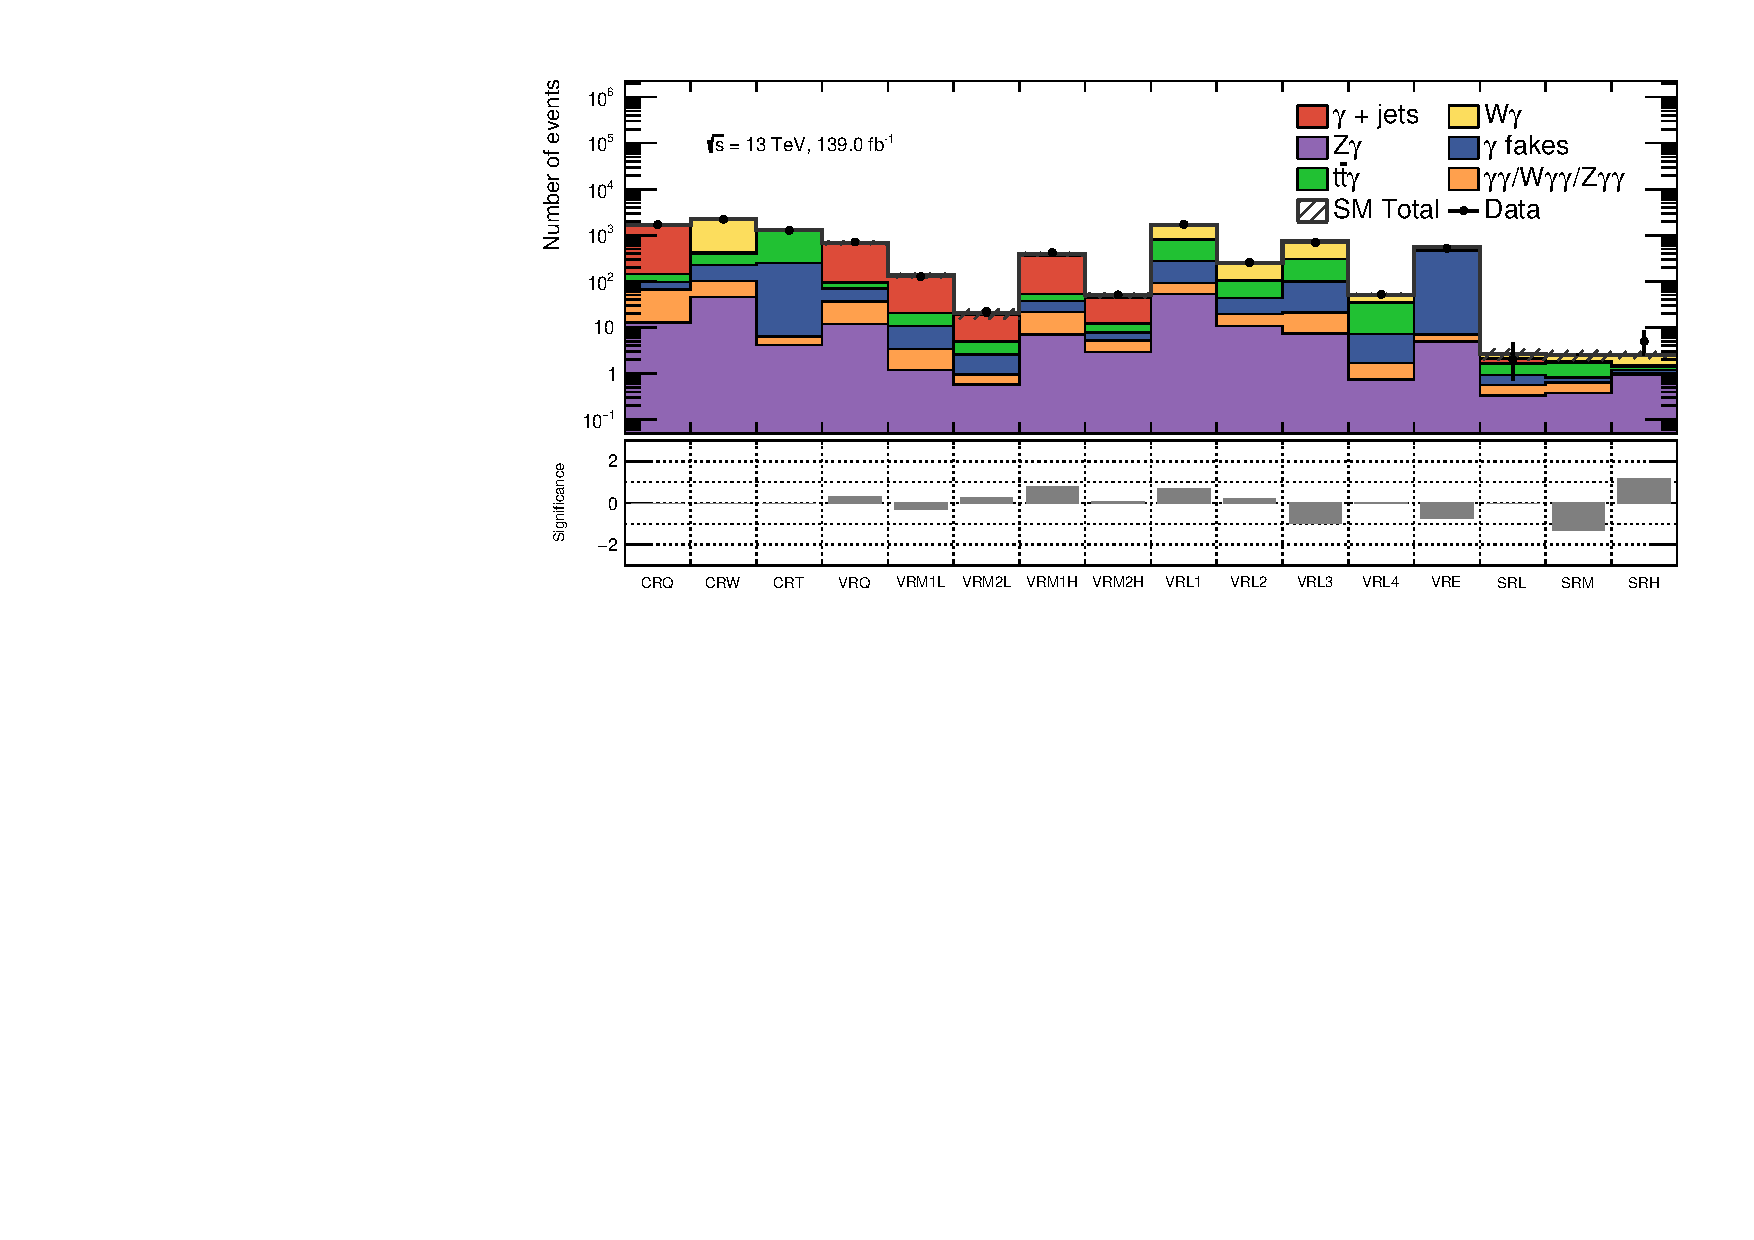
\includegraphics[width=0.89\textwidth]{images/results/fr2_unblind/regions_pull_significance.pdf}
  \caption{Resumen de la estimación de fondo y datos observados para cada región de control, validación y señal empleadas en el análisis. Abajo se muestra la diferencia entre el fondo estimado y los datos observados, en unidades de desviación estándar con respecto a la incertidumbre total del fondo.}
  \label{fig:regions_pulls_unblinded}
\end{figure}


\begin{figure}[!hb]
   \centering
   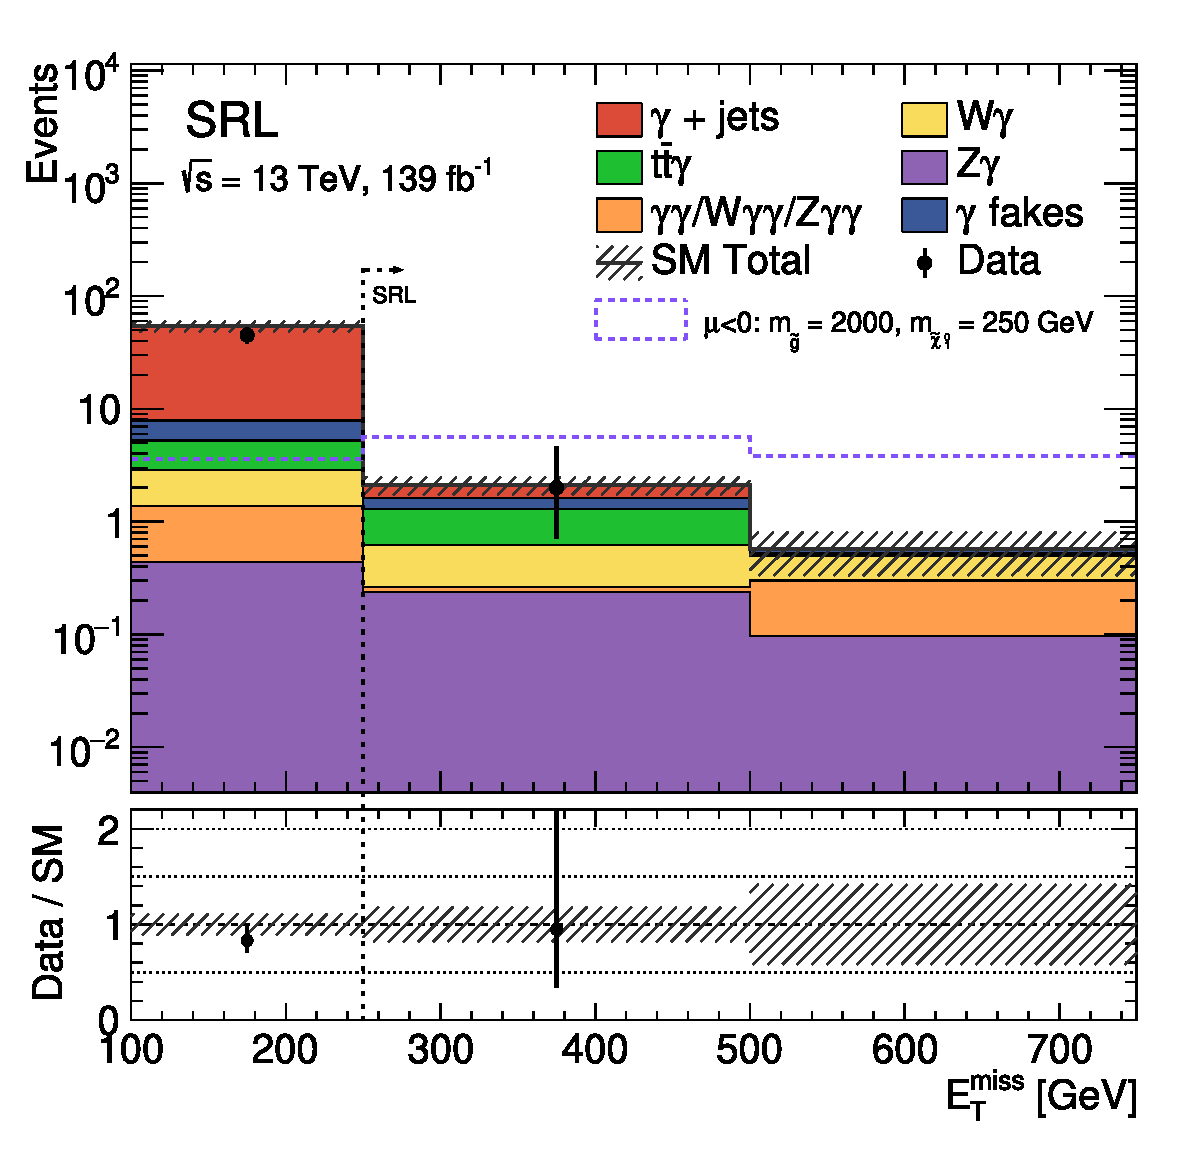
\includegraphics[width=0.48\textwidth]{images/results/fr2_unblind/sigReg_SRL_fr2_met_et_v2.pdf}
   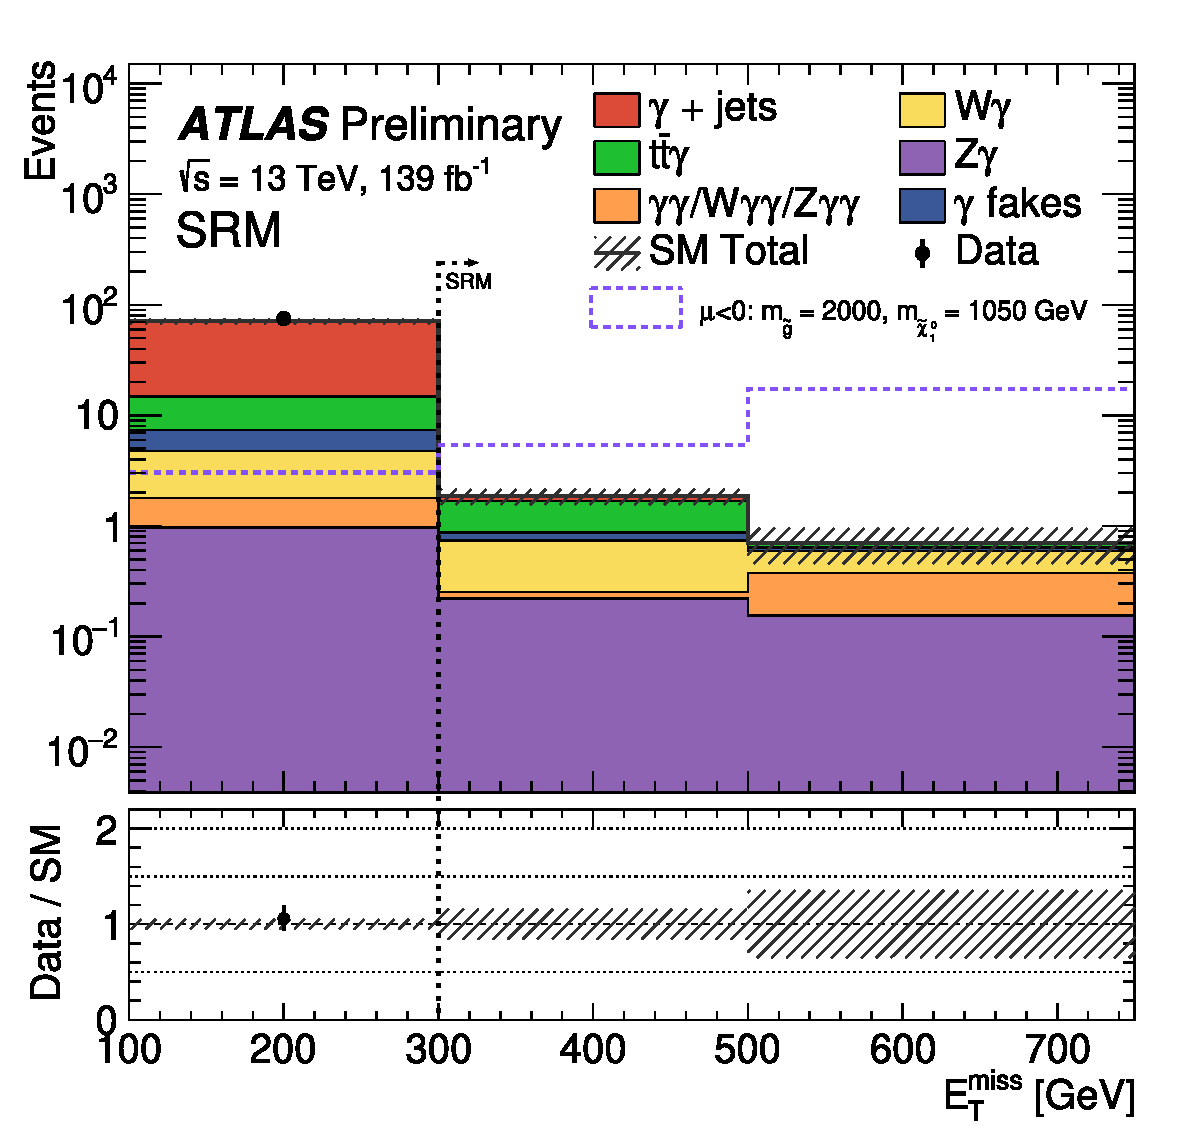
\includegraphics[width=0.48\textwidth]{images/results/fr2_unblind/sigReg_SRM_fr2_met_et_v2.pdf}
   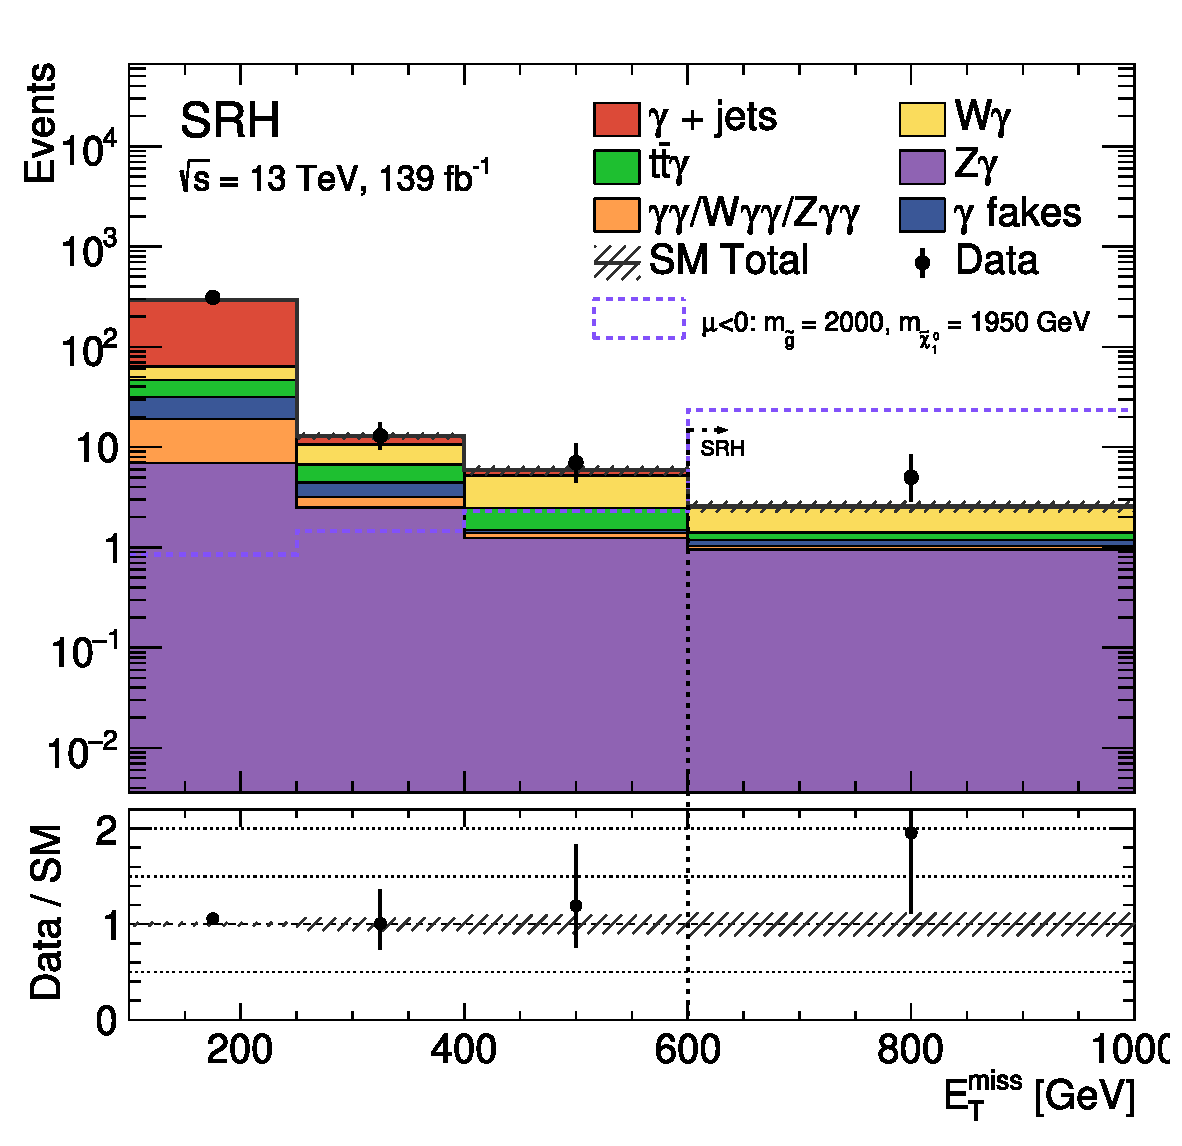
\includegraphics[width=0.48\textwidth]{images/results/fr2_unblind/sigReg_SRH_fr2_met_et_v2.pdf}
   \caption{Distribución de \met para los datos observados y la estimación de los fondos, en las regiones de señal SRL (izquierda), SRM (derecha) y SRH (abajo), omitiendo el corte en esa misma variable (N-1). Se incluye además la distribución del punto de señal más significativo para cada región.}
   \label{fig:met_n-1_SRL_SRM_SRH_fr2}
\end{figure}


% \solved{Falta la tabla de sistematicos} done

\begin{table}[ht!]
  \centering
  \caption{
  Resumen porcentual del aporte de las distintas incertezas sistemáticas en las regiones de señal, luego del ajuste de solo fondo. Debido a que las incertidumbres individuales pueden estar correlacionadas, la incertidumbre total no necesariamente es igual a la suma cuadrática de cada una.}
  %\resizebox{\textwidth}{!}{
    \begin{tabular}{lccc}
      \hline
      \hline
                                                  & SRL [\%] & SRM [\%] & SRH [\%] \\
      \hline
      \hline
      Incerteza total (estad.\ + sist.)           & 28       & 25       &  17  \\
      Incerteza estadística                    & 20       & 15       &  12  \\
      %Expected SM events & $2.67 \pm 0.54$ & $2.55 \pm 0.39$ & $2.55 \pm 0.31$ \\ %This uncertainty here is only statistical, because it was obtained without systematics.
      \hline
      Escala de energía y resolución de los jets             & 18       & 19       & 4.1  \\
      Calibración del $b$-tagging                       & 3.2     & 4.3     & 3.6  \\
      \textit{Jfakes}                                   & 2.1     & 2.5     & 2.3  \\
      Incertezas teóricas                                  & 3.6     & 3.1     & 10    \\
      \textit{Efakes}                              & 1.4     & 1.9     & $< 1$   \\
      Escala de energía y resolución de los electrones/fotones & 5.5     & 1.1     & 4.1  \\
      Reconstrucción e identificación de muones      & 2.6     & 1.8     & $< 1$   \\
      Identificación y aislamiento de fotones  & 2.6     & 2.1     & 1.1  \\
      Corrección por pile-up                         & $< 1$      & 1.2     & 1.0  \\
      Escala y resolución del término soft de \met & $< 1$      & $< 1$      & $< 1$   \\
      Luminosidad         & $< 1$      & $< 1$      & $< 1$   \\
      %                                             & SRL [\%] & SRM [\%] & SRH [\%] \\
      % \midrule
      % Total (stat. + syst.) uncertainty           & 28.0     & 24.9     &  17.4 \\
      % Statistical uncertainty                     & 20.2     & 15.3     &  12.2 \\
      % %Expected SM events & $2.67 \pm 0.54$ & $2.55 \pm 0.39$ & $2.55 \pm 0.31$ \\ %This uncertainty here is only statistical, because it was obtained without systematics.
      % \midrule
      % Jet energy scale and resolution             & 17.8    & 18.5    & 4.1  \\
      % b-tagging calibration                       & 3.2     & 4.3     & 3.6  \\
      % Jet fakes                                   & 2.1     & 2.5     & 2.3  \\
      % MC theory                                   & 3.6     & 3.1     & 10.2 \\
      % Electron fakes                              & 1.4     & 1.9     & < 1  \\
      % Electron/photon energy resolution and scale & 5.5     & 1.1     & 4.1  \\
      % Muon reconstruction and identification      & 2.6     & 1.8     & < 1  \\
      % Photon ID and isolation                     & 2.6     & 2.1     & 1.1  \\
      % Pile-up reweighting                         & < 1     & 1.2     & 1.0  \\
      % \MET\ soft-term scale and resolution        & < 1     & < 1     & < 1  \\
      \hline
      \hline
    \end{tabular}
  %}
\label{tab:syst_rel_impact}
\end{table}




\subsection{Límites independientes del modelo}


Dado el buen acuerdo entre la estimación del fondo y los datos observados en las distintas SRs, se establecen límites superiores en el número de eventos de cualquier fenómeno más allá del SM con el estado final del análisis. Los límites se establecen para cada SR con un nivel de confianza del 95\%, utilizando el estadístico de prueba definido en la Ecuación \ref{ec:st_qmu}, y las prescripciones para los $\text{CL}_{s}$ de la Ecuación \ref{eq:cls_limits}. Para ello se realiza un muestreo del número de eventos de señal para un cierto modelo, y se encuentra cuándo el valor de $\text{CL}_{s}$ cae por debajo del 5\%, método descripto en la Sección \ref{sec:flujo_busqueda}. La distribución de los distintos estadísticos de prueba se aproxima mediante la generación de {$\smallsim$}50000 toys.

En la Tabla \ref{tab:model_indep_ul} se muestran los límites superiores en el número de eventos en cada región de señal, tanto observados como esperados. Los límites observados son de $4.73$, $3$ y $7.55$ para las SRL, SRM y SRH respectivamente, lo que implica que cualquier modelo que prediga un número menor de eventos en dichas regiones, ya está excluido por el presente análisis. A su vez, se muestra el límite en la sección eficaz visible, obtenido a partir de dividir el anterior límite por la luminosidad total integrada, y multiplicarlo por la aceptancia (fracción de eventos que pasan todas las selecciones cinemáticas a nivel generador) y la eficiencia (fracción de esos eventos que pasan los cortes a nivel detector). 
% \tosolve{esto preguntar}
Se incluye el p-value de descubrimiento, que para regiones donde la predicción supera lo observado, se fija a un valor de $0.5$. En la región SRH el p-value es de $0.09$, lo que implica que las observaciones son compatibles con la hipótesis de <<solo fondo>>.


\begin{table}[!h]
  \centering
  \caption{Límites superiores en el número de eventos con un nivel de confianza del 95\% para cada región de señal, tanto observados como esperados. Adicionalmente se muestran los límites equivalentes en la sección eficaz visible, junto con el p-value de descubrimiento. Este último limitado a $0.5$ cuando el número de eventos observados es menor al esperado.}

    \begin{tabular}{lccccc}
    %\begin{tabular}{l|c|c|ccccc}
      \hline
      \hline
      Signal Region  & $S_{\mathrm{obs}}^{95}$  & $S_{\mathrm{exp}}^{95}$ & $\langle\epsilon{\sigma}\rangle_{\mathrm{obs}}^{95}$ [fb]  & $\langle\epsilon{\sigma}\rangle_{\mathrm{exp}}^{95}$ [fb] & $p_{0}$ ($Z$)\\
      \hline
      \hline
      SRL     &   4.73   &   $4.7^{+2.2}_{-1.2}$ &  0.034   &   $0.034^{+0.016}_{-0.009}$    &    0.50 (0.00)  \\ 
      SRM    &   3       &   $4.6^{+1.8}_{-1.1}$ &  0.022   &   $0.033^{+0.013}_{-0.008}$     &    0.50 (0.00)  \\ 
      SRH     &   7.55   &   $4.8^{+1.9}_{-1.4}$ &  0.054   &   $0.035^{+0.014}_{-0.010}$    &    0.09 (1.32)  \\
      \hline
      \hline
    \end{tabular}
    \label{tab:model_indep_ul}
  \end{table}



\subsection{Límites dependientes del modelo}


Se establecen los límites dependientes del modelo, buscando aquellos puntos del modelo de señal para los cuales $\text{CL}_{s}=0.05$, como se describe en la Sección \ref{sec:flujo_busqueda}. Dichos límites son calculados de forma independiente para cada región de señal, y luego combinados en un límite total. Para ello se elige de cada punto de señal, la región con mejor límite esperado, y se emplea su $\text{CL}_{s}$ para realizar la interpolación. La misma se realiza mediante el módulo \texttt{Scipy} \cite{2020SciPy-NMeth}, empleando la interpolación \texttt{multiquadratic} con el parámetro \texttt{smooth} igual a $0.1$. La distribución de los distintos estadísticos de prueba se aproxima mediante la generación de {$\smallsim$}50000 toys.

En la Figura \ref{fig:limit_plot_combined} se muestran los límites observados y esperados, combinando los resultados de las tres regiones de señal, para los que se incluye la variación de las incertezas sistemáticas en $\pm1\sigma$. Para los límites esperados se varían las incertezas experimentales, mientras que para los observados la incerteza en el cálculo de la sección eficaz del modelo. Estos límites excluyen a 95\% de intervalo de confianza la producción de gluinos con masas de hasta aproximadamente $2300\ \gev$, para la mayoría de las masas de neutralino estudiadas. 


\begin{figure}[ht!]
  \centering

  %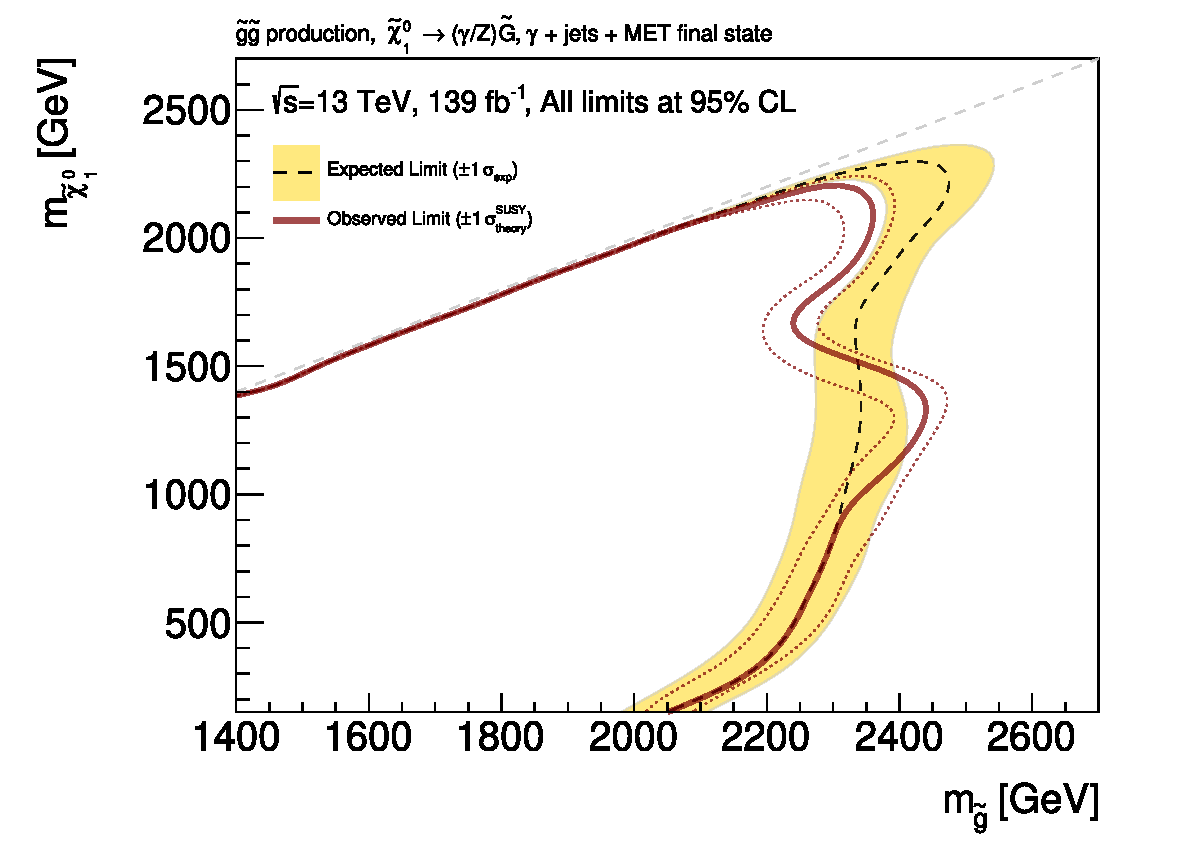
\includegraphics[width=0.45\textwidth]{figures/fr2_unblind/phjets_contour_plot_BestSR_wMatplotLib.pdf}
  % 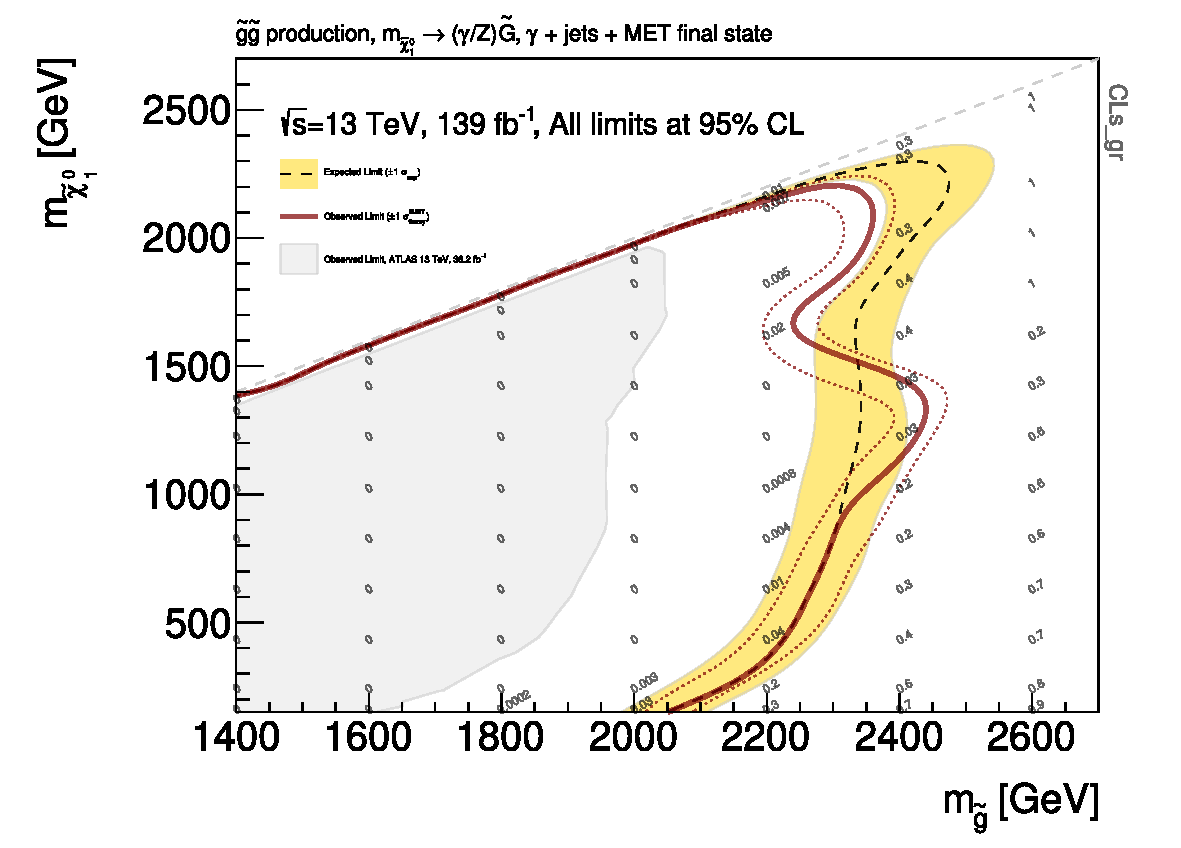
\includegraphics[width=0.45\textwidth]{figures/limits_plots/contour_plot_gZBestSR_wMatplotLib_full.pdf}
  %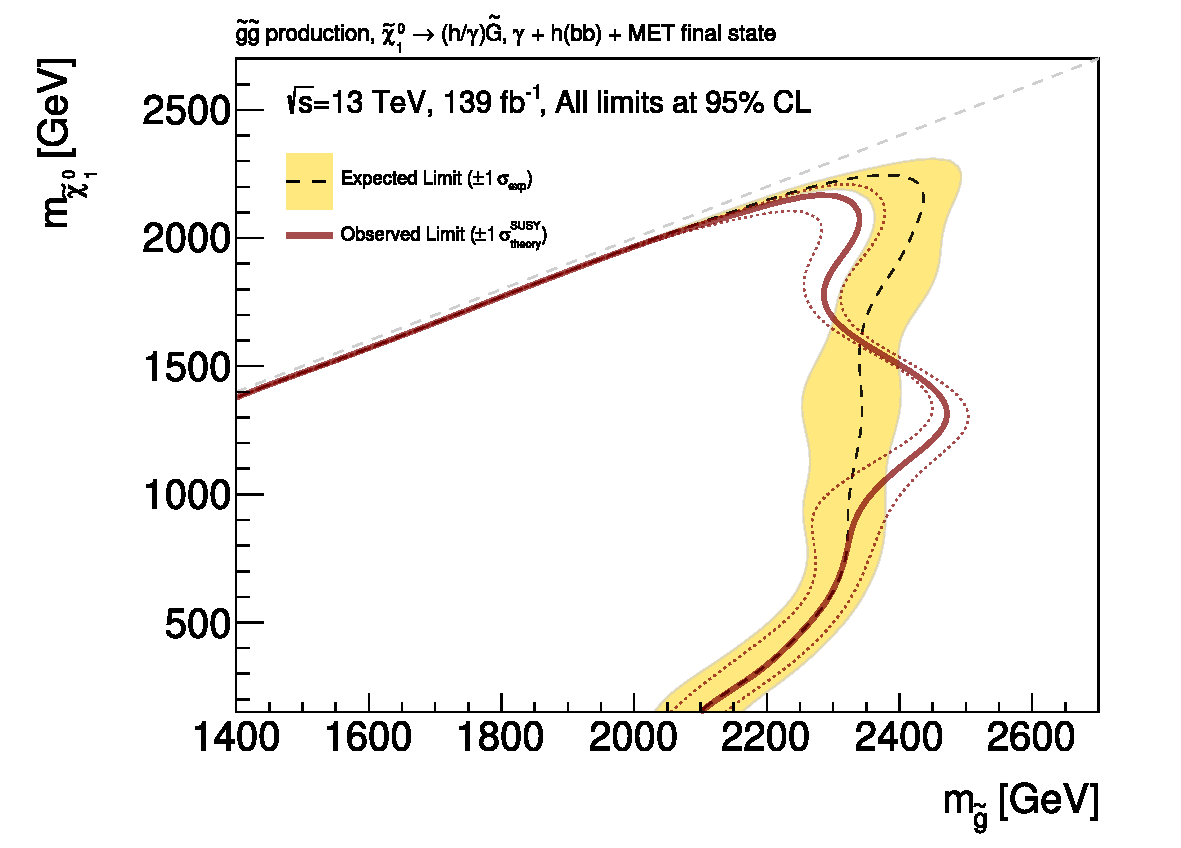
\includegraphics[width=0.45\textwidth]{figures/fr2_unblind/phb_contour_plot_BestSR_wMatplotLib.pdf}
  % \includegraphics[width=0.45\textwidth]{figures/limits_plots/contour_plot_gHBestSR_wMatplotLib_full.pdf}

  \includegraphics[width=0.9\textwidth]{images/results/limits_plots/contour_plot_gHBestSR_wMatplotLib_full.pdf}

  \caption{Límites observados (línea roja) y esperados (línea negra punteada) para una luminosidad integrada de $139\ \ifb$ a 95\% de intervalo de confianza, combinando los resultados de las tres regiones de señal. Las incertezas en los límites se obtienen variando en $\pm1\sigma$ las incertezas experimentales y en la sección eficaz de los puntos de señal. Los números en gris muestran el $\text{CL}_{s}$ para cada punto de señal.}
  \label{fig:limit_plot_combined}

\end{figure}
